%%
%% A Survey of Small Language Models for Agentic AI
%% ACM Journals (acmart) version -- content ported from paper_consolidated/paper.tex
%%
%% Build:  pdflatex -> bibtex -> pdflatex -> pdflatex
%%
%% -------------------------------------------------------------------------
%% Math fonts, set before the class is loaded.
%%
%% acmart's pdfLaTeX branch loads newtxmath with its libertine option, which
%% pulls the old Linux Libertine faces into every formula. We want Libertinus
%% throughout, so we mark newtxmath as already-loaded before acmart runs (its
%% \RequirePackage then becomes a no-op) and load libertinust1math instead,
%% which is the Libertinus-matched math font. Text, sans, mono and math then all
%% come from one family.
%%
%% If a future acmart release starts calling newtxmath-specific macros, drop
%% these two lines and the \usepackage{libertinust1math} below; the build falls
%% back to Libertinus text with Libertine-matched math, which is close but not
%% exact.
%% -------------------------------------------------------------------------
\expandafter\def\csname ver@newtxmath.sty\endcsname{9999/99/99}
%% Record the option acmart will ask for, so its \RequirePackage[libertine]
%% matches what LaTeX believes is already loaded and raises no option clash.
\expandafter\def\csname opt@newtxmath.sty\endcsname{libertine}

\documentclass[acmsmall,screen,review]{acmart}

%% -------------------------------------------------------------------------
%% Packages required by the ported section files
%% (acmart already provides amsmath, booktabs, graphicx, hyperref, natbib)
%% -------------------------------------------------------------------------
%% -------------------------------------------------------------------------
%% Fonts. acmart loads Libertine plus newtxmath by default; we replace that
%% whole stack with Libertinus, the maintained successor to Linux Libertine,
%% so that text, math, sans and mono all come from one family and the figures
%% (which set their text in Libertinus Serif via kaleido) match the body exactly.
%%
%% acmart has already loaded libertine + newtxmath by the time this file is
%% read, and both resist being unloaded, so we override rather than replace:
%% libertinus-type1 re-points the roman, sans and mono defaults at the
%% Libertinus Type 1 families. Math stays on newtxmath, which acmart configured
%% with its libertine option; since Libertinus is a direct fork of Linux
%% Libertine the math glyphs remain metrically and visually consistent with the
%% Libertinus text around them. Loading libertinust1math on top would clash with
%% newtxmath (duplicate \widebar, \txvec and friends) for no visible gain.
%% -------------------------------------------------------------------------
\usepackage{libertinus-type1}
\usepackage{libertinust1math}

%% acmart defines \liningnums in terms of \libertineLF, which would drag the old
%% Linux Libertine face back in for the few lining-figure runs that use it.
%% Point it at the Libertinus lining figures instead, so no Libertine glyph is
%% left anywhere in the document.
\AtEndPreamble{%
  \def\libertineLF{\LibertinusSerifLF}%
  \DeclareTextFontCommand{\liningnums}{\LibertinusSerifLF}%
}

%% Cross-references into the electronic supplement (supplement.tex), resolved
%% from its .aux file. Build order: main, supplement, main.
\usepackage{xr}
\externaldocument{less-is-more}
\newcommand{\suppsec}{Supplementary Section}

\usepackage{array}
\usepackage{multirow}
\usepackage{makecell}
\usepackage{tabularx}
\usepackage{longtable}
\usepackage{threeparttable}
\usepackage{adjustbox}
\usepackage{pdflscape}
\usepackage{tikz}
\usetikzlibrary{arrows.meta,positioning,fit,backgrounds,calc}

%% Acronyms / glossaries (same setup as the source manuscript)
\usepackage[acronym,nomain,nonumberlist,nopostdot]{glossaries}
\setacronymstyle{long-short}
%% No glossary is printed, so acronym uses must not become hyperlinks to it.
\glsdisablehyper

%% Column types used by the ported tables
\newcolumntype{C}[1]{>{\centering\arraybackslash}p{#1}}
\newcolumntype{L}[1]{>{\raggedright\arraybackslash}p{#1}}
\newcolumntype{R}[1]{>{\raggedleft\arraybackslash}p{#1}}
\newcolumntype{Y}{>{\raggedright\arraybackslash}X}

%% -------------------------------------------------------------------------
%% Evidence grading (Section 7.1.6). Each grade denotes the strongest kind of
%% source standing behind a claim, not the claim's importance.
%% -------------------------------------------------------------------------
% \textnormal resets any surrounding italic/bold before applying small caps, so
% the grade renders in every context (including inside \emph and table headers)
% without requesting a small-caps-italic shape that the text fonts lack.
\newcommand{\evgrade}[1]{\textnormal{\textsc{\small #1}}}
\newcommand{\evA}{\evgrade{A}}   % controlled: one harness, matched baselines
\newcommand{\evB}{\evgrade{B}}   % independent third-party evaluation
\newcommand{\evC}{\evgrade{C}}   % vendor self-reported
\newcommand{\evD}{\evgrade{D}}   % author interpretation / synthesis

%% \file{...} typesets a filename in typewriter and permits a line break after
%% each underscore, which plain \texttt does not; long script and dataset names
%% otherwise overrun the column.
\newcommand{\file}[1]{{\ttfamily\hyphenchar\font=-1
  \def\_{\char`\_\allowbreak}#1}}

\graphicspath{{figures/}}

% Acronym definitions for the glossaries package.
% Use \gls{key} in body prose: first use prints "Long form (SHORT)", later uses
% print "SHORT". \glspl{key} is the plural. Do NOT use \gls in section headings,
% figure/table captions, or table cells (first-use tracking misfires in floats).

% --- General ---
\newacronym{ai}{AI}{artificial intelligence}
\newacronym{ml}{ML}{machine learning}
\newacronym{nlp}{NLP}{natural language processing}
\newacronym{llm}{LLM}{large language model}
\newacronym{slm}{SLM}{small language model}
\newacronym{stem}{STEM}{science, technology, engineering, and mathematics}

% --- Architecture ---
\newacronym{moe}{MoE}{mixture of experts}
\newacronym{ssm}{SSM}{state-space model}
\newacronym{mha}{MHA}{multi-head attention}
\newacronym{mqa}{MQA}{multi-query attention}
\newacronym{gqa}{GQA}{grouped-query attention}
\newacronym{rope}{RoPE}{rotary position embeddings}
\newacronym{ffn}{FFN}{feed-forward network}
\newacronym{mlp}{MLP}{multi-layer perceptron}
\newacronym{kv}{KV}{key--value}

% --- Training and adaptation ---
\newacronym{kd}{KD}{knowledge distillation}
\newacronym{cot}{CoT}{chain of thought}
\newacronym{peft}{PEFT}{parameter-efficient fine-tuning}
\newacronym{lora}{LoRA}{low-rank adaptation}
\newacronym{qlora}{QLoRA}{quantized low-rank adaptation}
\newacronym{sft}{SFT}{supervised fine-tuning}
\newacronym{rlhf}{RLHF}{reinforcement learning from human feedback}
\newacronym{grpo}{GRPO}{group relative policy optimization}
\newacronym{rag}{RAG}{retrieval-augmented generation}
\newacronym{kl}{KL}{Kullback--Leibler}

% --- Compression ---
\newacronym{ptq}{PTQ}{post-training quantization}
\newacronym{qat}{QAT}{quantization-aware training}
\newacronym{awq}{AWQ}{activation-aware weight quantization}
\newacronym{gguf}{GGUF}{GPT-generated unified format}

% --- Hardware / deployment ---
\newacronym{gpu}{GPU}{graphics processing unit}
\newacronym{npu}{NPU}{neural processing unit}
\newacronym{cpu}{CPU}{central processing unit}
\newacronym{vram}{VRAM}{video memory}
\newacronym{tdp}{TDP}{thermal design power}
\newacronym{ttft}{TTFT}{time to first token}
\newacronym{sbc}{SBC}{single-board computer}
\newacronym{onnx}{ONNX}{Open Neural Network Exchange}

% --- Benchmarks / metrics ---
\newacronym{mmlu}{MMLU}{Massive Multitask Language Understanding}
\newacronym{gsm8k}{GSM8K}{Grade School Math 8K}
\newacronym{iqr}{IQR}{interquartile range}
\newacronym{kde}{KDE}{kernel density estimate}


%% -------------------------------------------------------------------------
%% Rights / journal metadata (placeholder values -- replace on submission)
%% -------------------------------------------------------------------------
\AtBeginDocument{\providecommand\BibTeX{{Bib\TeX}}}
%% No licence has been granted yet, so none is asserted on the review build.
%% Switch to \setcopyright{acmlicensed} once the ACM rights form is completed.
\setcopyright{none}
\copyrightyear{2026}
\acmYear{2026}
%% The DOI, volume, number, article number, and dates are assigned by ACM. For
%% the submission build the ACM reference block is suppressed and no date is
%% claimed.
\acmJournal{CSUR}
\settopmatter{printacmref=false}
%% No DOI is assigned before acceptance: clear acmart's placeholder and let
%% the footnote omit the DOI line when it is empty.
\acmDOI{}
\makeatletter
\def\@formatdoi#1{\edef\acmdoi@tmp{#1}\ifx\acmdoi@tmp\@empty\else\url{https://doi.org/#1}\fi}
\makeatother
\renewcommand{\thesection}{S\arabic{section}}
\renewcommand{\thefigure}{S\arabic{figure}}
\renewcommand{\thetable}{S\arabic{table}}

%% -------------------------------------------------------------------------
%% Front matter
%% -------------------------------------------------------------------------
\begin{document}

\title[A Survey of Small Language Models for Agentic AI: Supplement]{Supplementary Material for
  ``A Survey of Small Language Models for Agentic AI: Architectures, Compression,
  Deployment, and Evaluation''}

\author{Mohammed Gamal Ragab}
\authornote{Corresponding author.}
\orcid{0000-0001-5226-4962}
\email{mohammed.ragab@utp.edu.my}
\affiliation{%
  \department[0]{Department of Computer and Information Sciences}
  \department[1]{Center for Research in Data Science (CeRDaS)}
  \institution{Universiti Teknologi PETRONAS}
  \city{Seri Iskandar}
  \state{Perak}
  \country{Malaysia}
}

\author{Amgad Muneer}
\orcid{0000-0002-7157-3020}
\email{amabdulraheem@mdanderson.org}
\affiliation{%
  \department{Department of Imaging Physics}
  \institution{The University of Texas MD Anderson Cancer Center}
  \city{Houston}
  \state{Texas}
  \country{USA}
}

\renewcommand{\shortauthors}{Ragab and Muneer}

\begin{abstract}
  This electronic supplement contains the material referred to from the main
  text as Supplementary Sections S1--S18: the reporting dimensions and artifact
  vocabulary; the inclusion criteria, source verification, released artifacts,
  and update policy; the key model families; the technical background; the
  inventory figures; the taxonomy facets and architectural detail; compression
  methods and distillation variants; the audit protocol and coverage ledger;
  reference tables; deployment platforms; the conversion pipeline and routing
  designs; domain applications; model-level challenges; open research
  directions; the environmental accounting boundary; data provenance; and the
  generated variant inventory.
\end{abstract}

\begin{CCSXML}
<ccs2012>
   <concept>
       <concept_id>10010147.10010178.10010179</concept_id>
       <concept_desc>Computing methodologies~Natural language processing</concept_desc>
       <concept_significance>500</concept_significance>
   </concept>
   <concept>
       <concept_id>10010520.10010553</concept_id>
       <concept_desc>Computer systems organization~Embedded and cyber-physical systems</concept_desc>
       <concept_significance>300</concept_significance>
   </concept>
</ccs2012>
\end{CCSXML}

\ccsdesc[500]{Computing methodologies~Natural language processing}
\ccsdesc[300]{Computer systems organization~Embedded and cyber-physical systems}

\keywords{Small language models, agentic AI, model inventory, evaluation
  reporting, model compression}

\maketitle
\glsresetall

% Supplementary material: moved from Section 1.2 of the main text.

\section{Reporting Dimensions and Artifact Vocabulary}
\label{supp:definitions}

\subsection{Reporting Dimensions}
\label{subsubsec:intro_def_dimensions}

A single parameter count is not enough to determine whether a model will run on a
given device. Table~\ref{tab:reporting_dimensions} lists the dimensions this
survey reports where the primary source supplies them, and states which of them
each of our claims depends on. Where a source omits a dimension, the entry is
marked as not reported rather than estimated.

\begin{table}[t]
\centering
\caption{Reporting dimensions for a small language model, the deployment question each answers, and the coverage achieved across the 209-variant inventory. ``Derived'' means the value follows arithmetically from others rather than being reported.}
\label{tab:reporting_dimensions}
\footnotesize\adjustbox{max width=\linewidth}{%
\begin{tabular}{@{}lllc@{}}
\toprule
\textbf{Dimension} & \textbf{Question it answers} & \textbf{Bounds} & \textbf{Inventory coverage} \\
\midrule
Total parameters            & How large is the download? & C2 & 209/209 \\
Active parameters per token & What does one token cost? & C1 & 36/209 stated below total; else $=$ total \\
Weight memory at a precision & Will the weights fit? & C2 & Derived \\
Peak runtime memory          & Will it fit while running? & C2 & Not reported by vendors \\
FLOPs per token             & Compute cost per token & C1 & Derived (approximate) \\
KV-cache size per token     & Cost of long context & C1, C2 & Derived from head config \\
Context length              & Largest usable input & -- & 135/209 \\
Target hardware             & What did the vendor test on? & -- & Vendor-stated only \\
\bottomrule
\end{tabular}%
}
\end{table}

\subsection{Model-Artifact Vocabulary}
\label{subsubsec:intro_def_artifacts}

Because the inventory counts artifacts rather than papers, we also fix the
following. A \emph{family} is a named line of models sharing an architecture and
a training recipe (Qwen2.5, Gemma~3). A \emph{variant} is one released
parameter size within a family. Where a vendor publishes the base and the
post-trained checkpoint of that size in one release, the inventory records one
variant and marks its post-training status as ``both'' (63 of the 209); where
only one is published, or the two were released separately, the status is
recorded as that one. The post-training status is therefore a field of the
variant, not a second count. A \emph{checkpoint}
is a specific set of weights published under a version identifier; a variant may
be revised through several checkpoints, and the inventory records the variant,
not each checkpoint. A \emph{release} is a dated publication event covering one
or more variants. A \emph{pretrained} (or base) model is the artifact produced by
pretraining alone; an \emph{instruction-tuned} model has undergone supervised
instruction fine-tuning and usually a preference-optimization stage; a
\emph{reasoning-tuned} model has additionally been trained, by distillation of
long chain-of-thought traces, reinforcement learning, or both, to emit extended
intermediate reasoning before its answer. These three post-training statuses are
not interchangeable for evaluation purposes, which is why an evaluated artifact
must be identified to the checkpoint even though the inventory counts variants, and conflating them is one of the
specific defects in the public record documented in
Section~\ref{subsec:reported_overall}.

Two conventions follow from this vocabulary and are used consistently throughout.
Family names are written as their developers write them and with a space before
the version, as in Gemma~3, Qwen2.5, Phi-4, and Llama~3.2; the original 2023
LLaMA release keeps its own capitalization, since Meta renamed the line to
``Llama'' from Llama~2 onward. Checkpoint identifiers are written in the
hyphenated form used on the model hub, as in \texttt{Gemma-3-4B-it} or
\texttt{Qwen2.5-7B-Instruct}, and are used wherever the specific artifact rather
than the family is meant.


% Supplementary material: inclusion criteria, source verification, artifacts, update policy.

\section{Inclusion Criteria, Source Verification, Released Artifacts, and Update Policy}
\label{supp:method}

\subsection{Inclusion Criteria and Appraisal}
\label{subsubsec:intro_screening}

Inclusion criteria for the technique literature were: (T1)~the work concerns models at or below roughly twenty billion parameters, or a compression, adaptation, routing, or deployment technique whose evaluation includes that regime; (T2)~it is a peer-reviewed paper, an archived preprint, or a vendor technical report with a stable identifier; and (T3)~it reports enough methodological detail to determine what was measured.

Inclusion criteria for model variants were: (M1)~a source from the developer (technical report, paper, model card, model repository, or release announcement) that states the parameter count and architecture; (M2)~a public artifact or a documented evaluation card; (M3)~satisfaction of C1, with C2 status recorded separately; and (M4)~a dated release. Fine-tunes and merges of another party's checkpoint were excluded unless their developer released a technical report describing its own training recipe (as for the DeepSeek-R1-Distill models), as were quantized re-uploads, API aliases of a listed checkpoint, and variants differing only in serialization format.

\emph{What is computed and what is decided.} C1, C2, M1, and M4 are computed from recorded fields by \file{apply\_inclusion\_rules.py}: M1 from the stated parameter count and the field \texttt{developer\_source\_found} written by the source check below, and M4 from \texttt{release\_date\_precision}. Three kinds of exclusion are named editorial decisions listed in the script, because they cannot be computed from fields: encoder-decoder architecture (Flan-T5), derivative fine-tunes without a technical report (Nous Hermes~2 Mixtral, Vicuna-7B v1.5, Vicuna-13B, Jan-v1-4B), and an API alias (Mistral Tiny). Records whose size is undisclosed cannot be classified against C1 or C2; all of them, whatever their marketing (for example GPT-4o mini, Amazon Nova Micro and Lite, Claude Haiku, Gemini Flash-Lite, Nex-N2-Mini), are kept in the comparison part of the file with class \texttt{undisclosed} and are neither counted nor plotted as \glspl{slm} or \glspl{llm}. Release dates are recorded at the precision their sources give: day for 174 of the 209 included records, month for 22, and year for 13.

\emph{Appraisal of empirical works.} Works relied on for quantitative claims were appraised on whether they name the harness, state the evaluation conditions, report a matched baseline, and identify the evaluated checkpoint; the outcome, together with the reporting party's independence, is the evidence grade of Section~\ref{subsec:reported_grading}.

\subsection{Source Verification}
\label{subsec:source_verification}

On 8~October 2026, \file{verify\_sources.py} checked every included and excluded record, and every comparison record of stated size, against the Hugging Face Hub API: for each Hub repository a record links, it recorded whether the repository exists, its owner, creation date, licence tag, and the parameter count of its safetensors weights, and it classified the record's reference as a developer page, a paper, a Hub model page, or a secondary source (a model aggregator or press article). The result is written into each record (\texttt{source\_check}, \texttt{developer\_source\_found}) and into \file{source\_check\_log.csv}; Figure~\ref{fig:inventory_pipeline} places the check in the build process. Of the 209 included records, 197 link an existing repository owned by the developer and 12 link the developer's own announcement, paper, or code repository.

The check led to the following corrections, applied by \file{fix\_records\_v3\_6.py} and listed in the file's metadata. Twelve records whose reference was a model aggregator or a press article (the DeepSeek V4 Flash, Ling~3.0 Flash, Laguna, North Mini Code, Inkling Small, Nex-N2-Pro, Dots3-Note Preview, and Granite~4.0 Nano records) were re-sourced to the developer's Hub repository, with the original reference kept as \texttt{discovered\_via}; Ling~3.0 Flash Fin, recorded as API-only, is open-weight under MIT. Ling~3.0 Flash Sante, for which no developer source exists, fails M1 and was excluded. Voxtral Mini, previously excluded as undisclosed with a link to a different model, is the open-weight Voxtral Mini~3B (4.7B including its audio encoder, Apache~2.0) and was included. The BitNet b1.58 record, which described the 2024 paper but linked the 2025 checkpoint, now describes the released 2B4T model. The SmolLM2 records, which linked the SmolLM3 page, the Mistral~7B v0.3 release date (2024, not 2023), and the Granite~4.1 references were corrected. For nine records the ratio of the Hub parameter count to the vendor's nominal size falls outside 0.8--1.25 (for example Gemma~2-2B, nominal 2B, Hub 2.6B; Qwen2.5-Omni-7B, Hub 10.7B including its audio components; BitNet b1.58 2B4T, whose ternary weights are stored packed); the recorded size is the vendor's statement, the Hub count is kept in the log, and none of the differences changes a record's C1 or C2 status.

\begin{figure}[t]
\centering
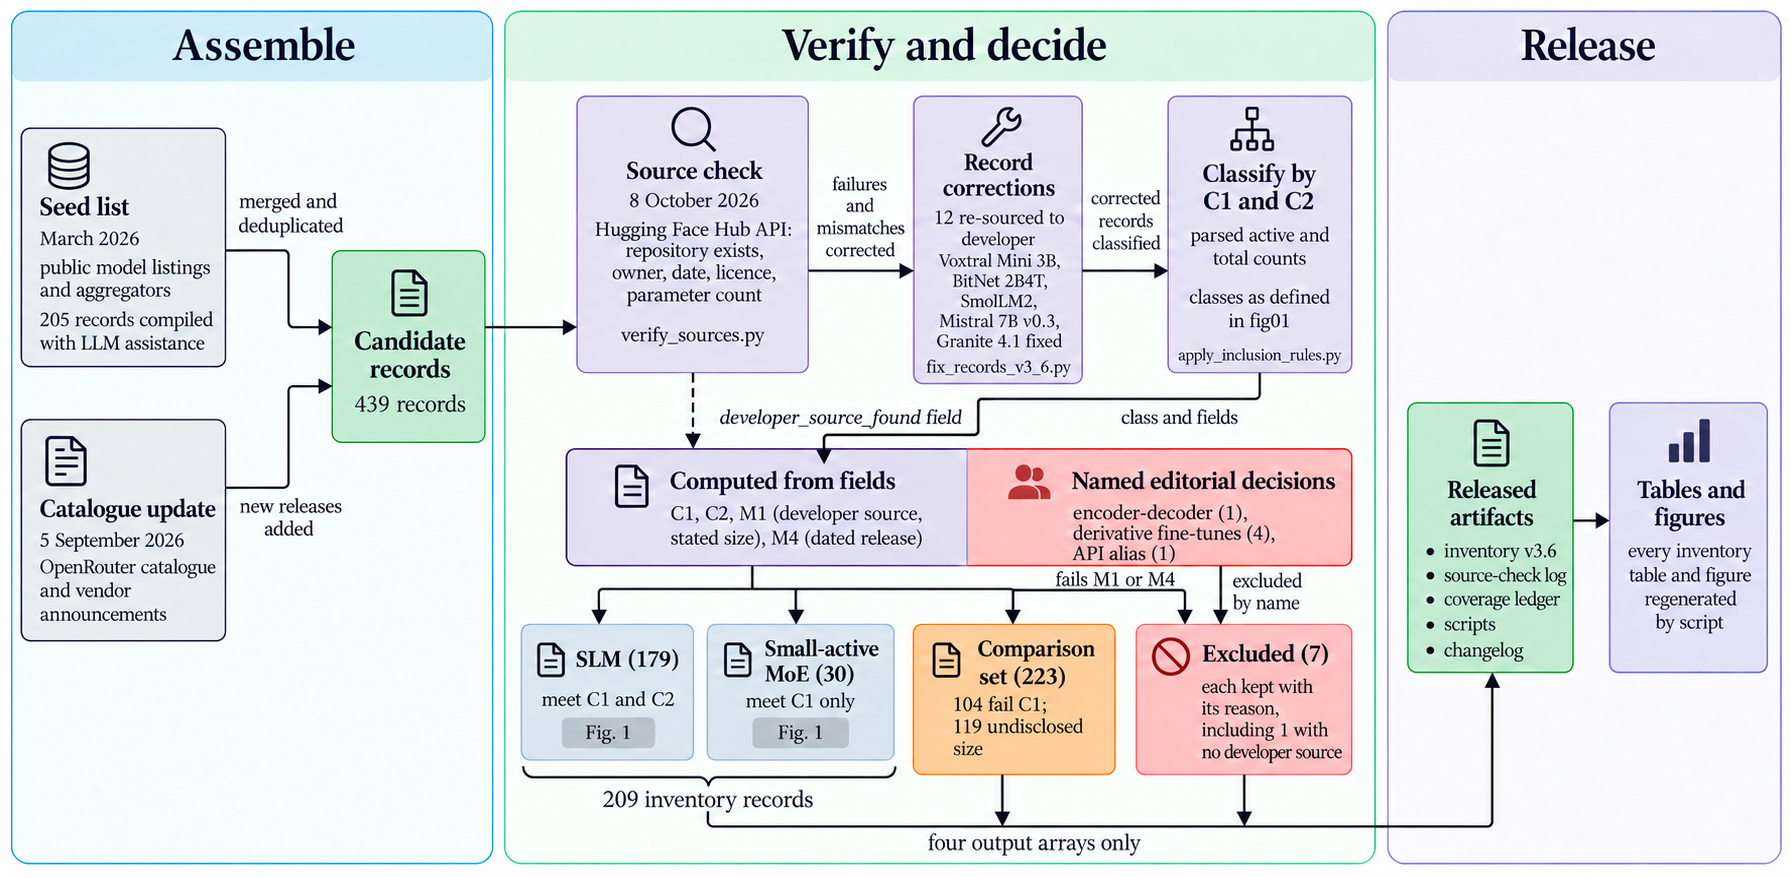
\includegraphics[width=\linewidth]{fig02-inventory-pipeline.png}
\caption{How the inventory was assembled, verified, and filtered. Secondary listings only seeded the candidate list; every record was then checked against its developer source and corrected where needed. C1, C2, M1, and M4 are computed from recorded fields; the encoder-decoder, derivative, and alias exclusions are named editorial decisions. All four arrays, the source-check log, the coverage ledger, the scripts, and the changelog are released.}
\Description{Flow diagram in four columns. Assemble: seed list (March 2026) and catalogue update (September 2026) feed 439 candidate records. Verify: source check against the Hugging Face Hub (October 2026), record corrections, and classification by C1 and C2. Decide: decisions computed from fields, and named editorial exclusions. Arrays: SLM 179, small-active mixture of experts 30, comparison 223 (104 fail C1, 119 undisclosed), and excluded 7. All outputs lead to the released artifacts.}
\label{fig:inventory_pipeline}
\end{figure}

\subsection{Count History}
\label{subsec:count_history}

Earlier drafts reported 126 variants. Version~3.3 of the inventory added 27 releases from May to September 2026 (153). Version~3.4 placed records by the rule rather than by how they had been filed: 64 models meeting C1 had been filed outside the \gls{slm} inventory and two 24B dense models inside it (215). Version~3.5 corrected a parser that had read the total in place of the active count for five legacy \gls{moe} records and removed eleven records by the inclusion criteria (209: 178 \glspl{slm} and 31 small-active-parameter \glspl{moe}). Version~3.6 applied the source verification above: Voxtral Mini~3B entered as an \gls{slm} and Ling~3.0 Flash Sante left, and the four records of undisclosed size that version~3.5 had excluded as ``vendor-positioned small'' were moved to the comparison set with every other undisclosed record (209: 179 \glspl{slm} and 30 small-active-parameter \glspl{moe}; 223 comparison records, of which 104 are of disclosed size and fail C1 and 119 are undisclosed; 7 excluded). The changelog in the released file names every record added, moved, or removed at each step.

\subsection{Released Artifacts}
\label{subsec:intro_artifacts}

The following are released with the paper: the inventory \file{merged\_llm\_database.json} (version~3.6), with one record per variant carrying its parameter counts, C1/C2 status, class, inclusion decision and reason, developer source, source-check result and date, and the excluded and comparison records alongside; the source-check log \file{source\_check\_log.csv}; the audit coverage ledger \file{audit\_coverage\_ledger.csv} (\suppsec~\ref{subsec:audit_ledger}); the scripts that correct and verify records, apply the inclusion rule, build the ledger, and generate every inventory table and figure; and the changelog. They are provided as supplementary files with the submission and will be deposited in a versioned archival repository under a persistent identifier, so that the exact snapshot underlying this paper, and any later one, can be retrieved.

\subsection{Snapshot and Update Policy}
\label{subsubsec:intro_snapshot}

This paper reports model releases through 4~September 2026, as recorded in version~3.6 of the inventory (8~October 2026). Releases appearing between submission and acceptance are added to the released inventory and recorded in the changelog, and are discussed in the text only where they change a conclusion; tables and figures are regenerated from the inventory at the last revision before acceptance. Works appearing during review that bear on RQ2--RQ5 are added to the synthesis, as was done for one study published after the snapshot \citep{laskar2026sftrl}. The released artifact is the authority on what the inventory contained at any given date.

% Supplementary material: moved from Section 2.4 of the main text.

\section{Key SLM Families}
\label{supp:families}

\subsection{Microsoft Phi Series}
\label{subsubsec:phi_series}
The Phi series represents Microsoft's systematic exploration of data-quality-driven model development. Phi-1 (1.3B) \citep{gunasekar2023phi1} demonstrated strong code generation performance through training on synthetic ``textbook-quality'' data. Phi-2 (2.7B) \citep{microsoft2023phi2} extended this to general language understanding. Phi-3-mini (3.8B) \citep{abdin2024phi3} formalized the approach with 3.3 trillion training tokens, reporting 68.8\% on \gls{mmlu} (5-shot) and 82.5\% on \gls{gsm8k} (8-shot, chain-of-thought) for the instruction-tuned checkpoint (\evC). Phi-3.5-mini \citep{abdin2024phi35} added 128K context length support with improved multilingual capabilities. Phi-4 (14B) \citep{abdin2024phi4} introduced a fundamentally enhanced training pipeline incorporating ${\sim}40\%$ synthetic data, reporting 84.8\% on \gls{mmlu} and 80.4\% on MATH under OpenAI's simple-evals settings, and reporting that it exceeds its teacher GPT-4o on several STEM benchmarks (\evC). Phi-4-mini (3.8B) \citep{microsoft2025phi4mini} updated the architecture with \gls{gqa} (24 query, 8 \gls{kv} heads), a 200K-token vocabulary, and training on 5 trillion tokens, reporting 88.6\% on \gls{gsm8k} (8-shot, chain-of-thought; \evC). Phi-4-reasoning \citep{abdin2025phi4reasoning} is Phi-4 after supervised fine-tuning on curated prompts with o3-mini reasoning demonstrations; Phi-4-reasoning-plus adds a short phase of outcome-based reinforcement learning. Both are reported to outperform DeepSeek-R1-Distill-Llama-70B and to approach the full DeepSeek-R1 on AIME~2025 (\evC).

\subsection{Google Gemma Series}
\label{subsubsec:gemma_series}
Google's Gemma family \citep{gemma2024} derives from the Gemini model architecture and training infrastructure. Gemma 1 offered 2B and 7B variants trained on 3T and 6T tokens respectively, using Multi-Query Attention (MQA) for the 2B model and standard Multi-Head Attention for the 7B. Gemma 2 \citep{gemma2team2024} introduced significant architectural improvements: local-global interleaved attention layers, logit soft-capping, and knowledge distillation for the 2B and 9B variants (from a larger teacher model). The pre-trained Gemma 2-9B reports 71.3\% on \gls{mmlu} (5-shot; \evC). Gemma 3 \citep{team2025gemma3} further advanced the architecture with a 5:1 local-to-global attention interleaving ratio (reducing the sliding window from 4096 to 1024 tokens) and replaced the logit soft-capping of Gemma 2 with QK-norm. Gemma 3 distills all model sizes from larger teachers and introduces a 1B variant whose instruction-tuned checkpoint reports 48.0\% on MATH, close to the 49.4\% of the instruction-tuned Gemma 2-9B with $9\times$ fewer parameters (\evC).

\subsection{Alibaba Qwen Series}
\label{subsubsec:qwen_series}
The Qwen2 \citep{yang2024qwen2} and Qwen2.5 \citep{qwen2024qwen25} families from Alibaba are trained on up to 18 trillion tokens, far beyond Chinchilla-optimal ratios. Qwen2.5 offers models at 0.5B, 1.5B, 3B, 7B, 14B, 32B, and 72B parameters, all sharing a consistent GQA-based architecture with \gls{rope} and SwiGLU activations. The pre-trained 3B model reports 65.6\% on \gls{mmlu} (5-shot), 79.1\% on \gls{gsm8k}, and 42.6\% on MATH (both 4-shot) (\evC); its developers credit the STEM and code share of the training data for its mathematics and coding results.

\subsection{Other Significant SLM Families}
\label{subsubsec:other_slm_families}
TinyLlama (1.1B) \citep{zhang2024tinyllama} adopted the Llama 2 architecture and tokenizer and trained on about 1 trillion tokens of SlimPajama and StarCoder data for roughly three epochs, showing that extended training of very small models continues to pay. Mistral 7B \citep{jiang2023mistral} combined grouped-query attention, introduced by \citet{ainslie2023gqa}, with sliding-window attention in a 7.3B-parameter model, and reports outperforming Llama 2 13B while being $1.8\times$ smaller. Meta's Llama 3.2 \citep{meta2024llama32} released 1B and 3B models for edge and mobile devices, derived from Llama~3.1 8B by pruning and distillation, trained on up to 9 trillion tokens with 128K context. SmolLM2 (135M, 360M, 1.7B) \citep{allal2025smollm2} from Hugging Face trained on 11 trillion tokens of carefully curated data. H2O-Danube (1.8B) \citep{singer2024h2odanube} introduced sliding window attention in a compact model trained on 1 trillion tokens. OLMo 2 (1B, 7B, 13B) \citep{olmo2025} from AI2 was released as a fully open model (data, code, weights, and training logs), achieving competitive performance through QK-norm and carefully staged training. StableLM-2 (1.6B) \citep{stabilityai2024stablelm} was trained on about 2 trillion tokens (counting repeated epochs) of multilingual data. The BLOOM family (560M, 1.1B, 1.7B, 3B, 7.1B) \citep{bloom2022} remains notable as a multilingual model trained on 46 languages using ALiBi positional encoding, though its 350B-token training budget is modest by current standards.



% Supplementary material: moved from Sections 2.2, 2.3 and 2.5 of the main text.

\section{Training, Compression, and Deployment Background}
\label{supp:background}

\subsection{Knowledge Distillation and Model Compression}
\label{subsec:background_distillation}
Knowledge distillation, first formalized by \citet{hinton2015distilling}, transfers knowledge from a large ``teacher'' model to a smaller ``student'' by training the student to match the teacher's soft probability distributions (logits) rather than hard labels. This approach preserves the teacher's learned representations of inter-class similarities, information that is lost in one-hot labels, and has proven remarkably effective in the \gls{llm} era. Modern distillation strategies for language models encompass several complementary approaches.

Logit-based distillation trains the student to minimize the KL divergence between its output distribution and the teacher's softened distribution, parameterized by a temperature $\tau$. Google's Gemma 2 \citep{gemma2team2024} and Gemma 3 \citep{team2025gemma3} employ this approach extensively: all Gemma 3 model sizes, including the 27B variant, are trained using knowledge distillation from a larger teacher. The distillation loss is combined with a standard next-token prediction loss, with the relative weighting serving as a key hyperparameter. Feature-based distillation \citep{romero2015fitnets} additionally aligns intermediate representations between teacher and student, capturing structural knowledge that may not be fully expressed in output logits. Microsoft's Orca 2 \citep{mitra2023orca2} demonstrated a variant where a smaller model is taught to use different reasoning strategies depending on task complexity, outperforming models with 5--$10\times$ more parameters on reasoning benchmarks.

Synthetic data generation represents an increasingly dominant form of implicit distillation. Rather than direct logit matching, a powerful \gls{llm} (e.g., GPT-4, Claude 3.5) generates high-quality training examples that are then used to train smaller models. The Phi series pioneered this approach with the ``Textbooks Are All You Need'' methodology \citep{gunasekar2023phi1}, generating synthetic textbook-style content with carefully controlled complexity and diversity. Phi-4's training data is reported to be about 40\% synthetic, generated across 50 dataset types including multi-agent conversations and structured reasoning chains \citep{abdin2024phi4} (\evC); its developers attribute much of its STEM performance to this data, an attribution that has not been tested in a controlled comparison against web-corpus training at equal compute. Post-training quantization, pruning, and adaptation methods are reviewed in \suppsec~\ref{supp:compression}; together with distillation during training they form the usual \gls{slm} optimization pipeline.

\subsection{Efficient Fine-Tuning Methods}
\label{subsec:background_efficient_finetuning}
Full fine-tuning updates all model parameters using task-specific data, which for a 7B-parameter model can require tens of gigabytes of accelerator memory once gradients and optimizer states are included. This cost has made \gls{peft} central to the practical adaptation of \glspl{slm}, particularly when the target deployment environment is a single GPU or an edge-oriented workstation.

\gls{lora} \citep{hu2022lora} addresses this constraint by freezing the pretrained backbone and learning low-rank update matrices for selected linear layers. For a weight matrix $W_0 \in \mathbb{R}^{d \times k}$, the update is parameterized as $\Delta W = BA$, where $B \in \mathbb{R}^{d \times r}$ and $A \in \mathbb{R}^{r \times k}$ with rank $r \ll \min(d,k)$. This drastically reduces the number of trainable parameters while preserving the ability to specialize a model for downstream tasks. \gls{qlora} \citep{dettmers2023qlora} extends this idea by quantizing the frozen base model to 4-bit NormalFloat (NF4) precision and training the adapters in higher precision, allowing models that would ordinarily require multi-GPU setups to be fine-tuned on a single high-memory accelerator.

Beyond LoRA-style adapters, the \gls{peft} landscape includes prompt-based and prefix-based adaptation strategies that shift task information into learned soft prompts or attention prefixes rather than updating the backbone itself. These approaches can be attractive when multiple lightweight task specializations must be maintained simultaneously. However, they tend to underperform LoRA-family methods on complex reasoning tasks, where direct adaptation of attention and feed-forward projections provides a stronger inductive bias for task transfer.

The choice between prompting and fine-tuning therefore depends on task specificity, data availability, and deployment constraints. In-context learning offers zero-training adaptation and is well suited to broad tasks when labeled data are scarce, but it consumes context length and raises inference latency. By contrast, \gls{peft} methods incur an upfront training cost yet reduce per-query overhead and typically yield larger gains on narrow or reasoning-heavy tasks. Prompting and \gls{qlora} results are rarely reported under matched conditions, so they cannot be compared across models from the published record; measuring them is one of the verification studies proposed in Section~\ref{subsec:challenges_verification}.


\subsection{Edge AI and On-Device Inference}
\label{subsec:background_edge_ai}
The edge AI inference stack has matured rapidly, transforming \gls{slm} deployment from a research exercise to a production-ready capability. The llama.cpp framework \citep{gerganov2023llamacpp} is the most widely used runtime for CPU and mixed CPU-GPU inference, and the one against which the others in Table~\ref{tab:deployment_frameworks} position themselves, supporting the \gls{gguf} quantization format with dozens of precision variants (Q2\_K through Q8\_0). Its ecosystem includes llamafile (single-executable packaging), Ollama (user-friendly serving), and extensive platform support spanning x86, ARM, Apple Silicon, and NVIDIA GPUs. Benchmarking on single-board computers shows that llamafile achieves up to $4\times$ higher throughput and 30--40\% lower power consumption than Ollama for equivalent models \citep{nguyen2025sbc}.

Meta's ExecuTorch \citep{meta2024executorch} is an on-device runtime with a small base runtime and backends for CoreML, Qualcomm QNN, ARM, MediaTek, and Vulkan; Meta used it for the on-device measurements of its Llama~3.2 1B and 3B models \citep{meta2024llama32card}. MLC-LLM \citep{mlc2024} deploys through ML compilation (TVM) to iOS, Android, web, and embedded GPUs. ONNX Runtime \citep{microsoft2019onnx} provides cross-platform deployment with optimization passes for diverse hardware. WebLLM \citep{webllm2024} runs inference in the browser with WebGPU and reports retaining up to 80\% of native performance (\evC). Google's LiteRT (formerly TensorFlow Lite) targets mobile CPUs, GPUs, and \glspl{npu} \citep{google2025litert}; its vendor-reported speedups on Qualcomm \glspl{npu} are measured against CPU execution on the vendor's chosen models and are not comparable with the other figures here.

The fundamental constraint in edge deployment is memory bandwidth rather than compute. Flagship phones and mainstream laptops offer on the order of 50--100~GB/s of memory bandwidth, unified-memory laptop designs considerably more, and single-board computers well under 30~GB/s, versus 2--3~TB/s for datacenter GPUs \citep{xu2024device}. Single-stream autoregressive decoding reads the full weight set once per generated token, so in that regime it is bandwidth-bound and quantization from 16 to 4 bits converts a storage saving into a decode-time saving roughly in proportion to the bandwidth freed. The proportionality is regime-dependent rather than general: it weakens under batching as arithmetic intensity rises, largely disappears during the compute-bound prefill phase, and is reduced further on hardware without native low-precision kernels. Section~\ref{subsec:deployment_calc_vs_meas} sets out the conditions in full. Because single-stream interactive use is the dominant on-device regime, INT4 quantization is nevertheless a performance enabler there and not only a storage optimization.



% Supplementary material: inventory figures referred to from Section 3 of the main text.

\section{Inventory Figures}
\label{supp:figures}

The figures below are generated from version~3.6 of the released inventory (releases through 4~September 2026) and are referred to from Section~\ref{sec:taxonomy} of the main text. Unless stated otherwise, they cover the 209 inventory records, that is, the 179 \glspl{slm} and the 30 small-active-parameter \glspl{moe}. Figure~\ref{fig:releases_by_size} gives releases by size band, Figure~\ref{fig:family_size_range} the size span of the principal families, Figure~\ref{fig:context_by_year} context length by year, Figure~\ref{fig:moe_vs_dense} the dense and \gls{moe} split, and Figure~\ref{fig:modality} supported modalities.

\begin{figure}[t]
  \centering
  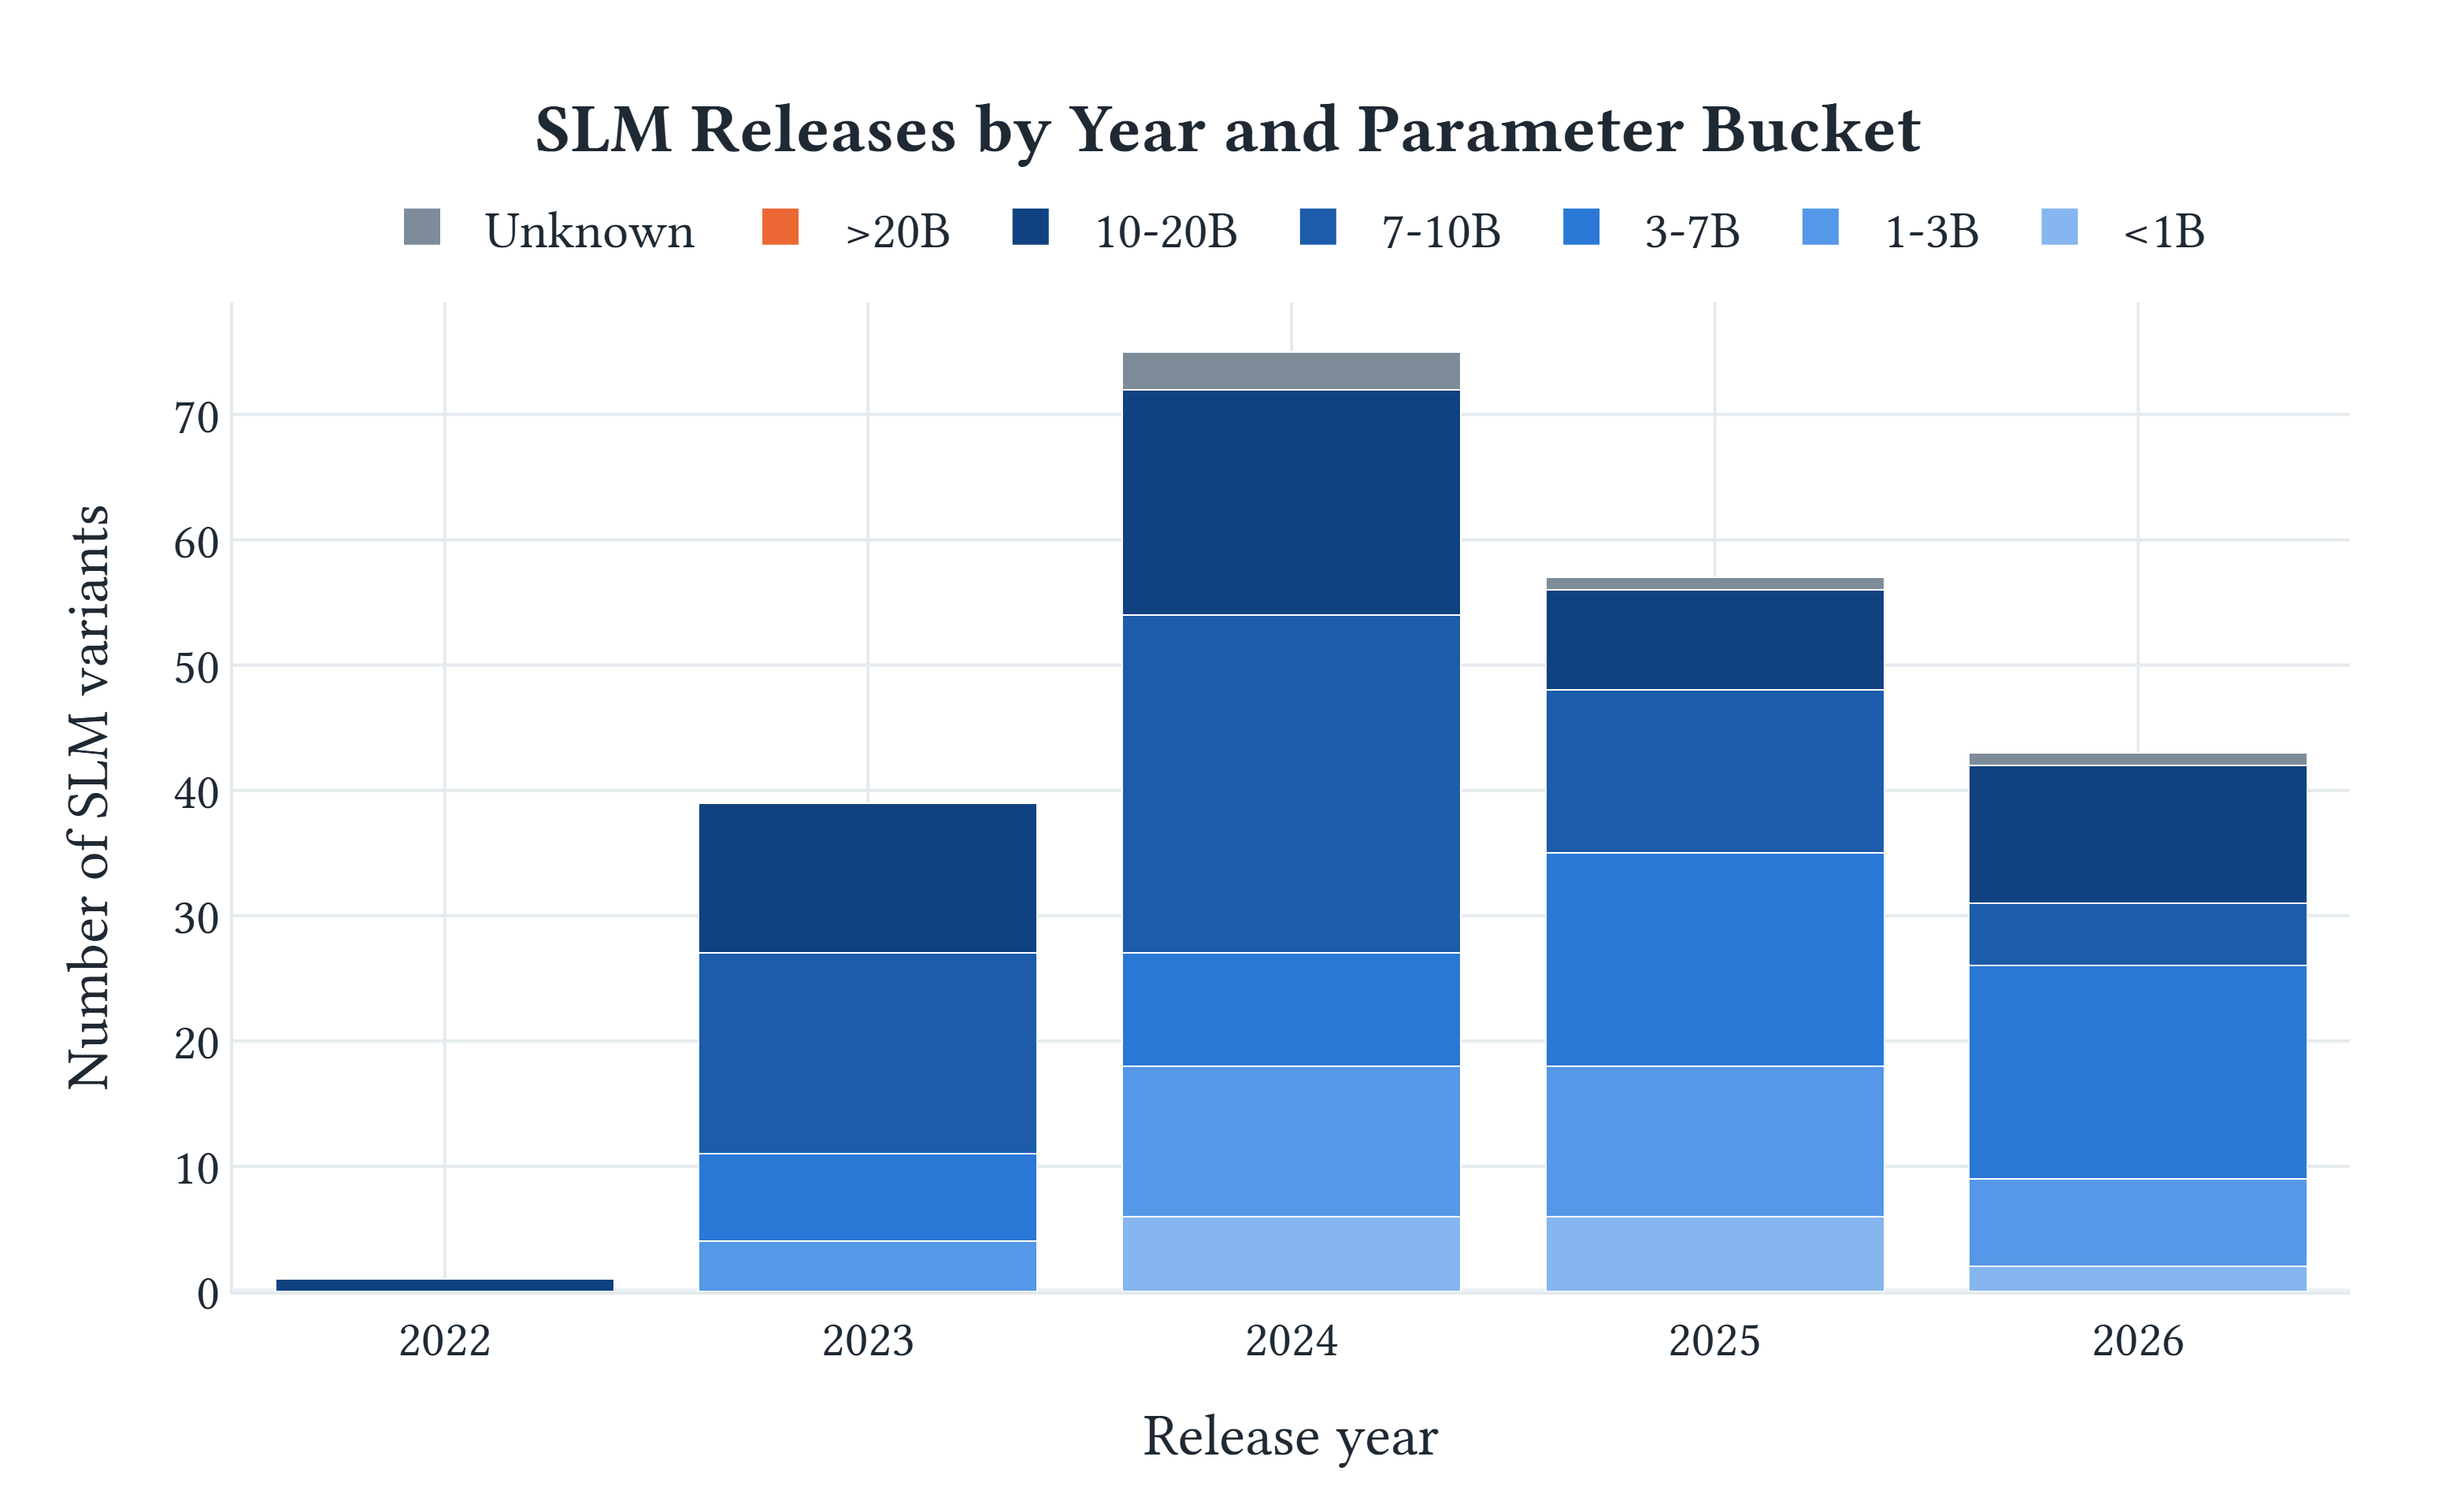
\includegraphics[width=\linewidth]{paper_slm_releases_by_size.png}
  \caption{Inventory variants by release year and total-parameter band (2026 to 4~September). The 7--10B band is the largest in 2023, 2024, and 2025; the sub-1B and 1--3B bands appear in numbers from 2024; in 2026 the largest band is the one above 20B total, which consists of small-active-parameter MoEs.}
  \Description{Stacked bar chart of inventory releases per year, split by total-parameter band. The 7-10B band is the largest from 2023 to 2025; sub-1B and 1-3B releases appear in numbers from 2024; in 2026 the band above 20B total parameters, made up of small-active-parameter mixtures of experts, is the largest.}
  \label{fig:releases_by_size}
\end{figure}

\begin{figure}[t]
  \centering
  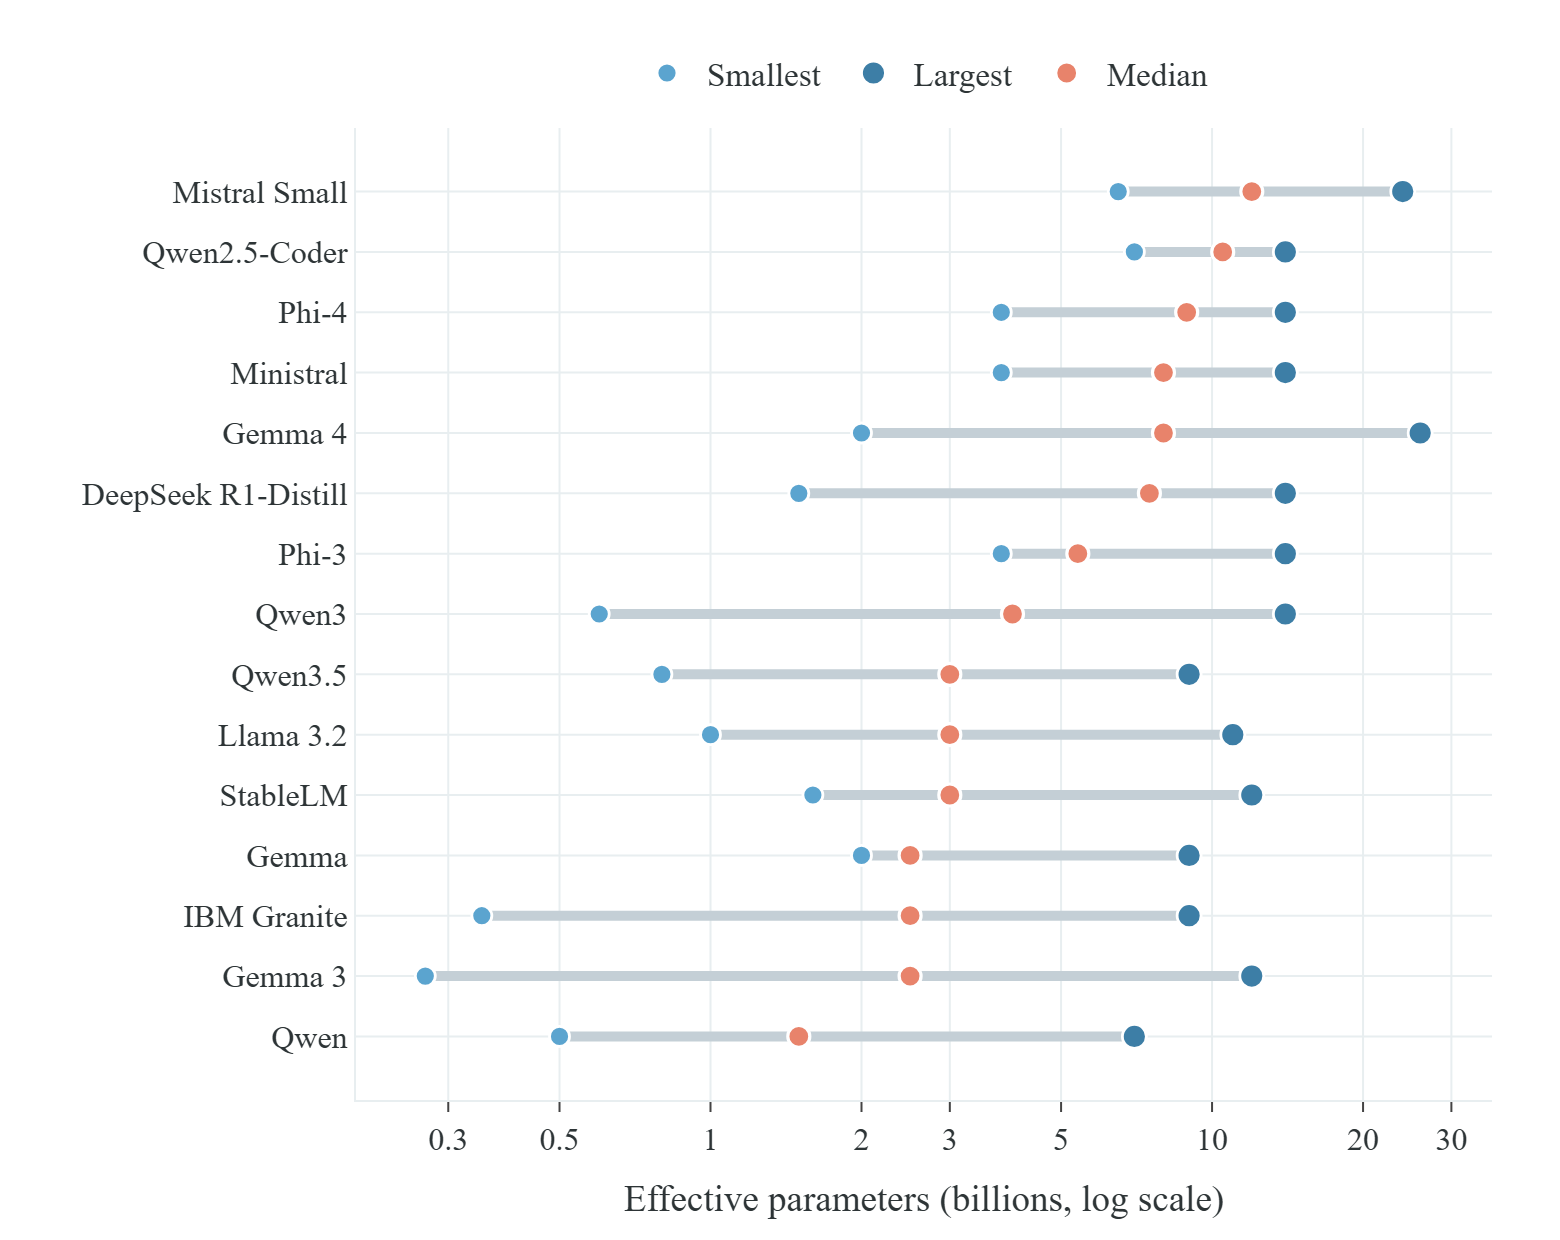
\includegraphics[width=\linewidth]{paper_slm_family_size_range.png}
  \caption{Parameter span (minimum, median, maximum, in billions, log scale) of the principal families in the inventory.}
  \Description{Horizontal range plot on a logarithmic axis showing the minimum, median, and maximum parameter count in billions for each principal family.}
  \label{fig:family_size_range}
\end{figure}

\begin{figure}[t]
  \centering
  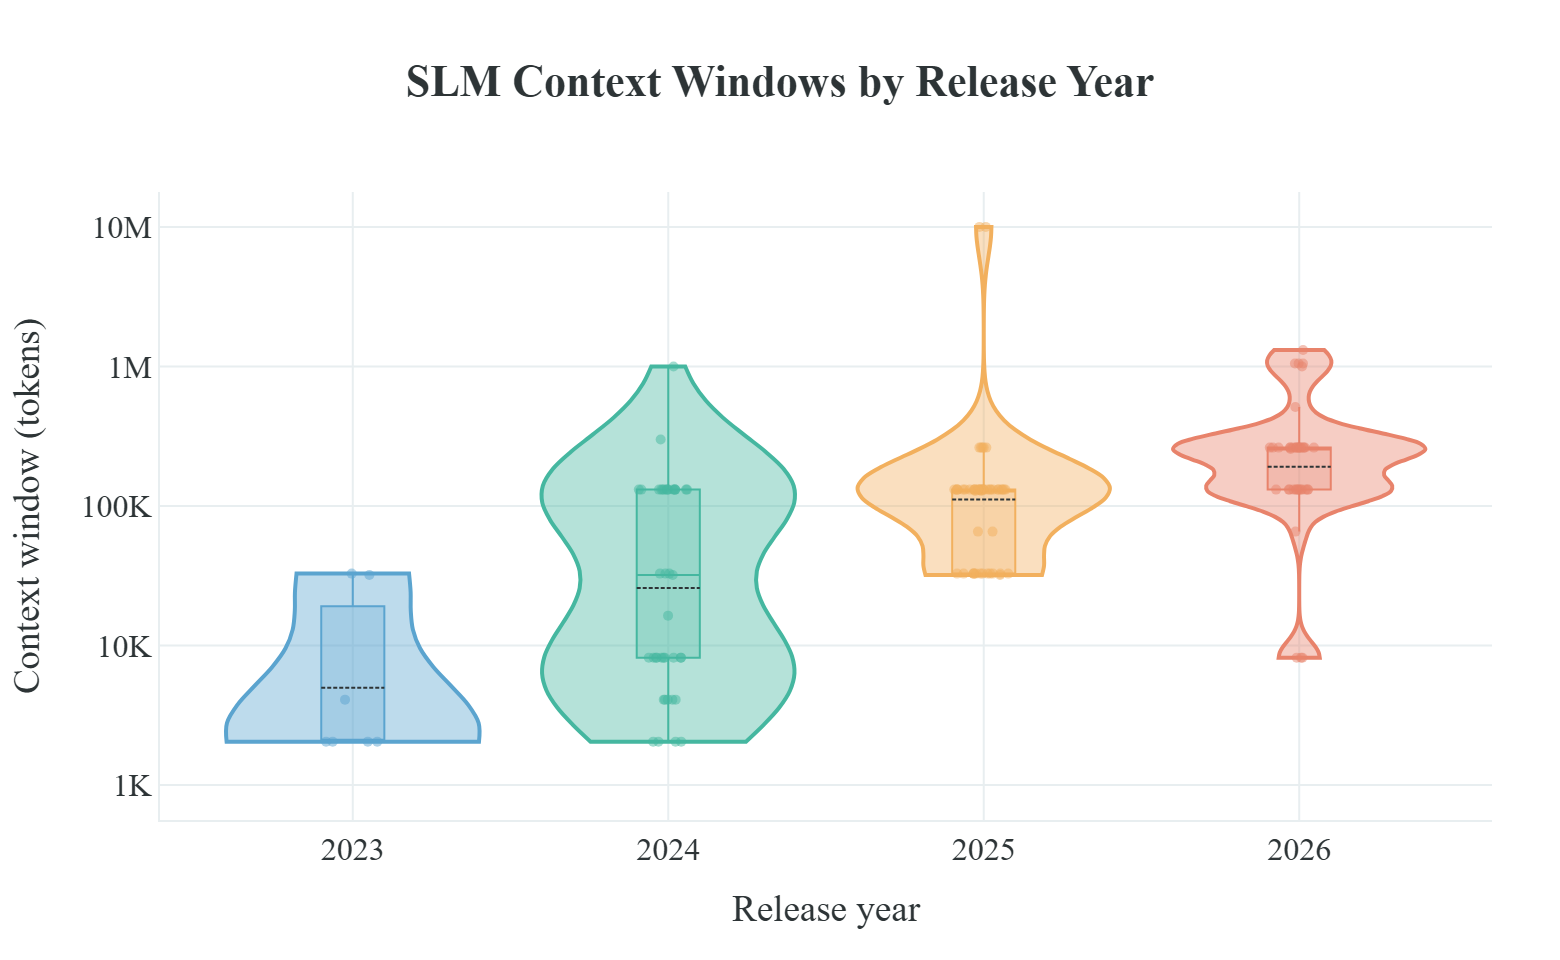
\includegraphics[width=\linewidth]{paper_slm_context_by_year.png}
  \caption{Supported context window of inventory variants by release year (log scale), for the records that state one: 5 of 36 in 2023, 39 of 74 in 2024, 52 of 58 in 2025, and 39 of 41 in 2026. Each violin is a kernel-density estimate; the inner box marks the interquartile range, the dashed line the mean, and the dots individual models. Because 2023 coverage is thin and 2026 includes small-active-parameter MoEs, the trend is indicative.}
  \Description{Violin plot of supported context window on a logarithmic axis against release year. The distribution shifts upward from a few thousand tokens in 2023 to a median of about one hundred thousand tokens or more from 2025.}
  \label{fig:context_by_year}
\end{figure}

\begin{figure}[t]
  \centering
  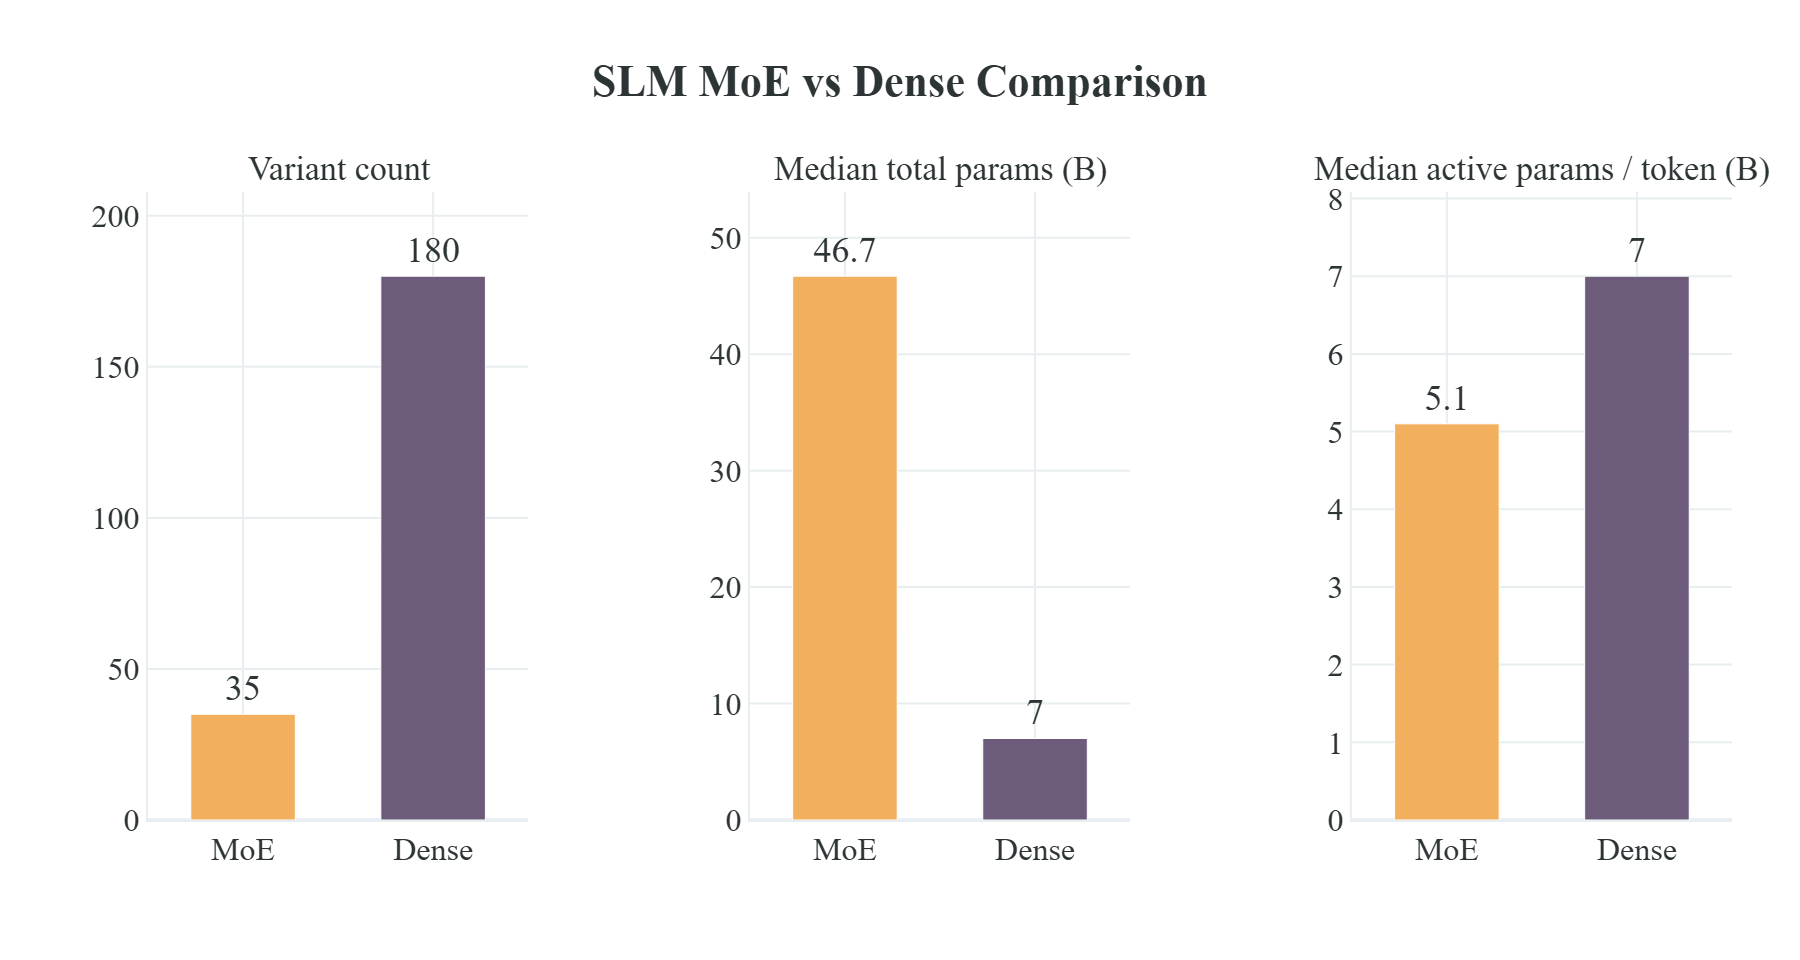
\includegraphics[width=\linewidth]{paper_slm_moe_vs_dense.png}
  \caption{Mixture-of-experts versus dense variants in the inventory: variant count (left), median total parameters (centre), and median \emph{active} parameters per token (right). MoE models carry a much larger total parameter count at a per-token cost comparable to dense models, which is the distinction between conditions C1 and C2.}
  \Description{Three side-by-side bar charts comparing mixture-of-experts and dense variants on count, median total parameters, and median active parameters per token. Dense models are far more numerous; mixture-of-experts models carry much larger totals at comparable active counts.}
  \label{fig:moe_vs_dense}
\end{figure}

\begin{figure}[t]
  \centering
  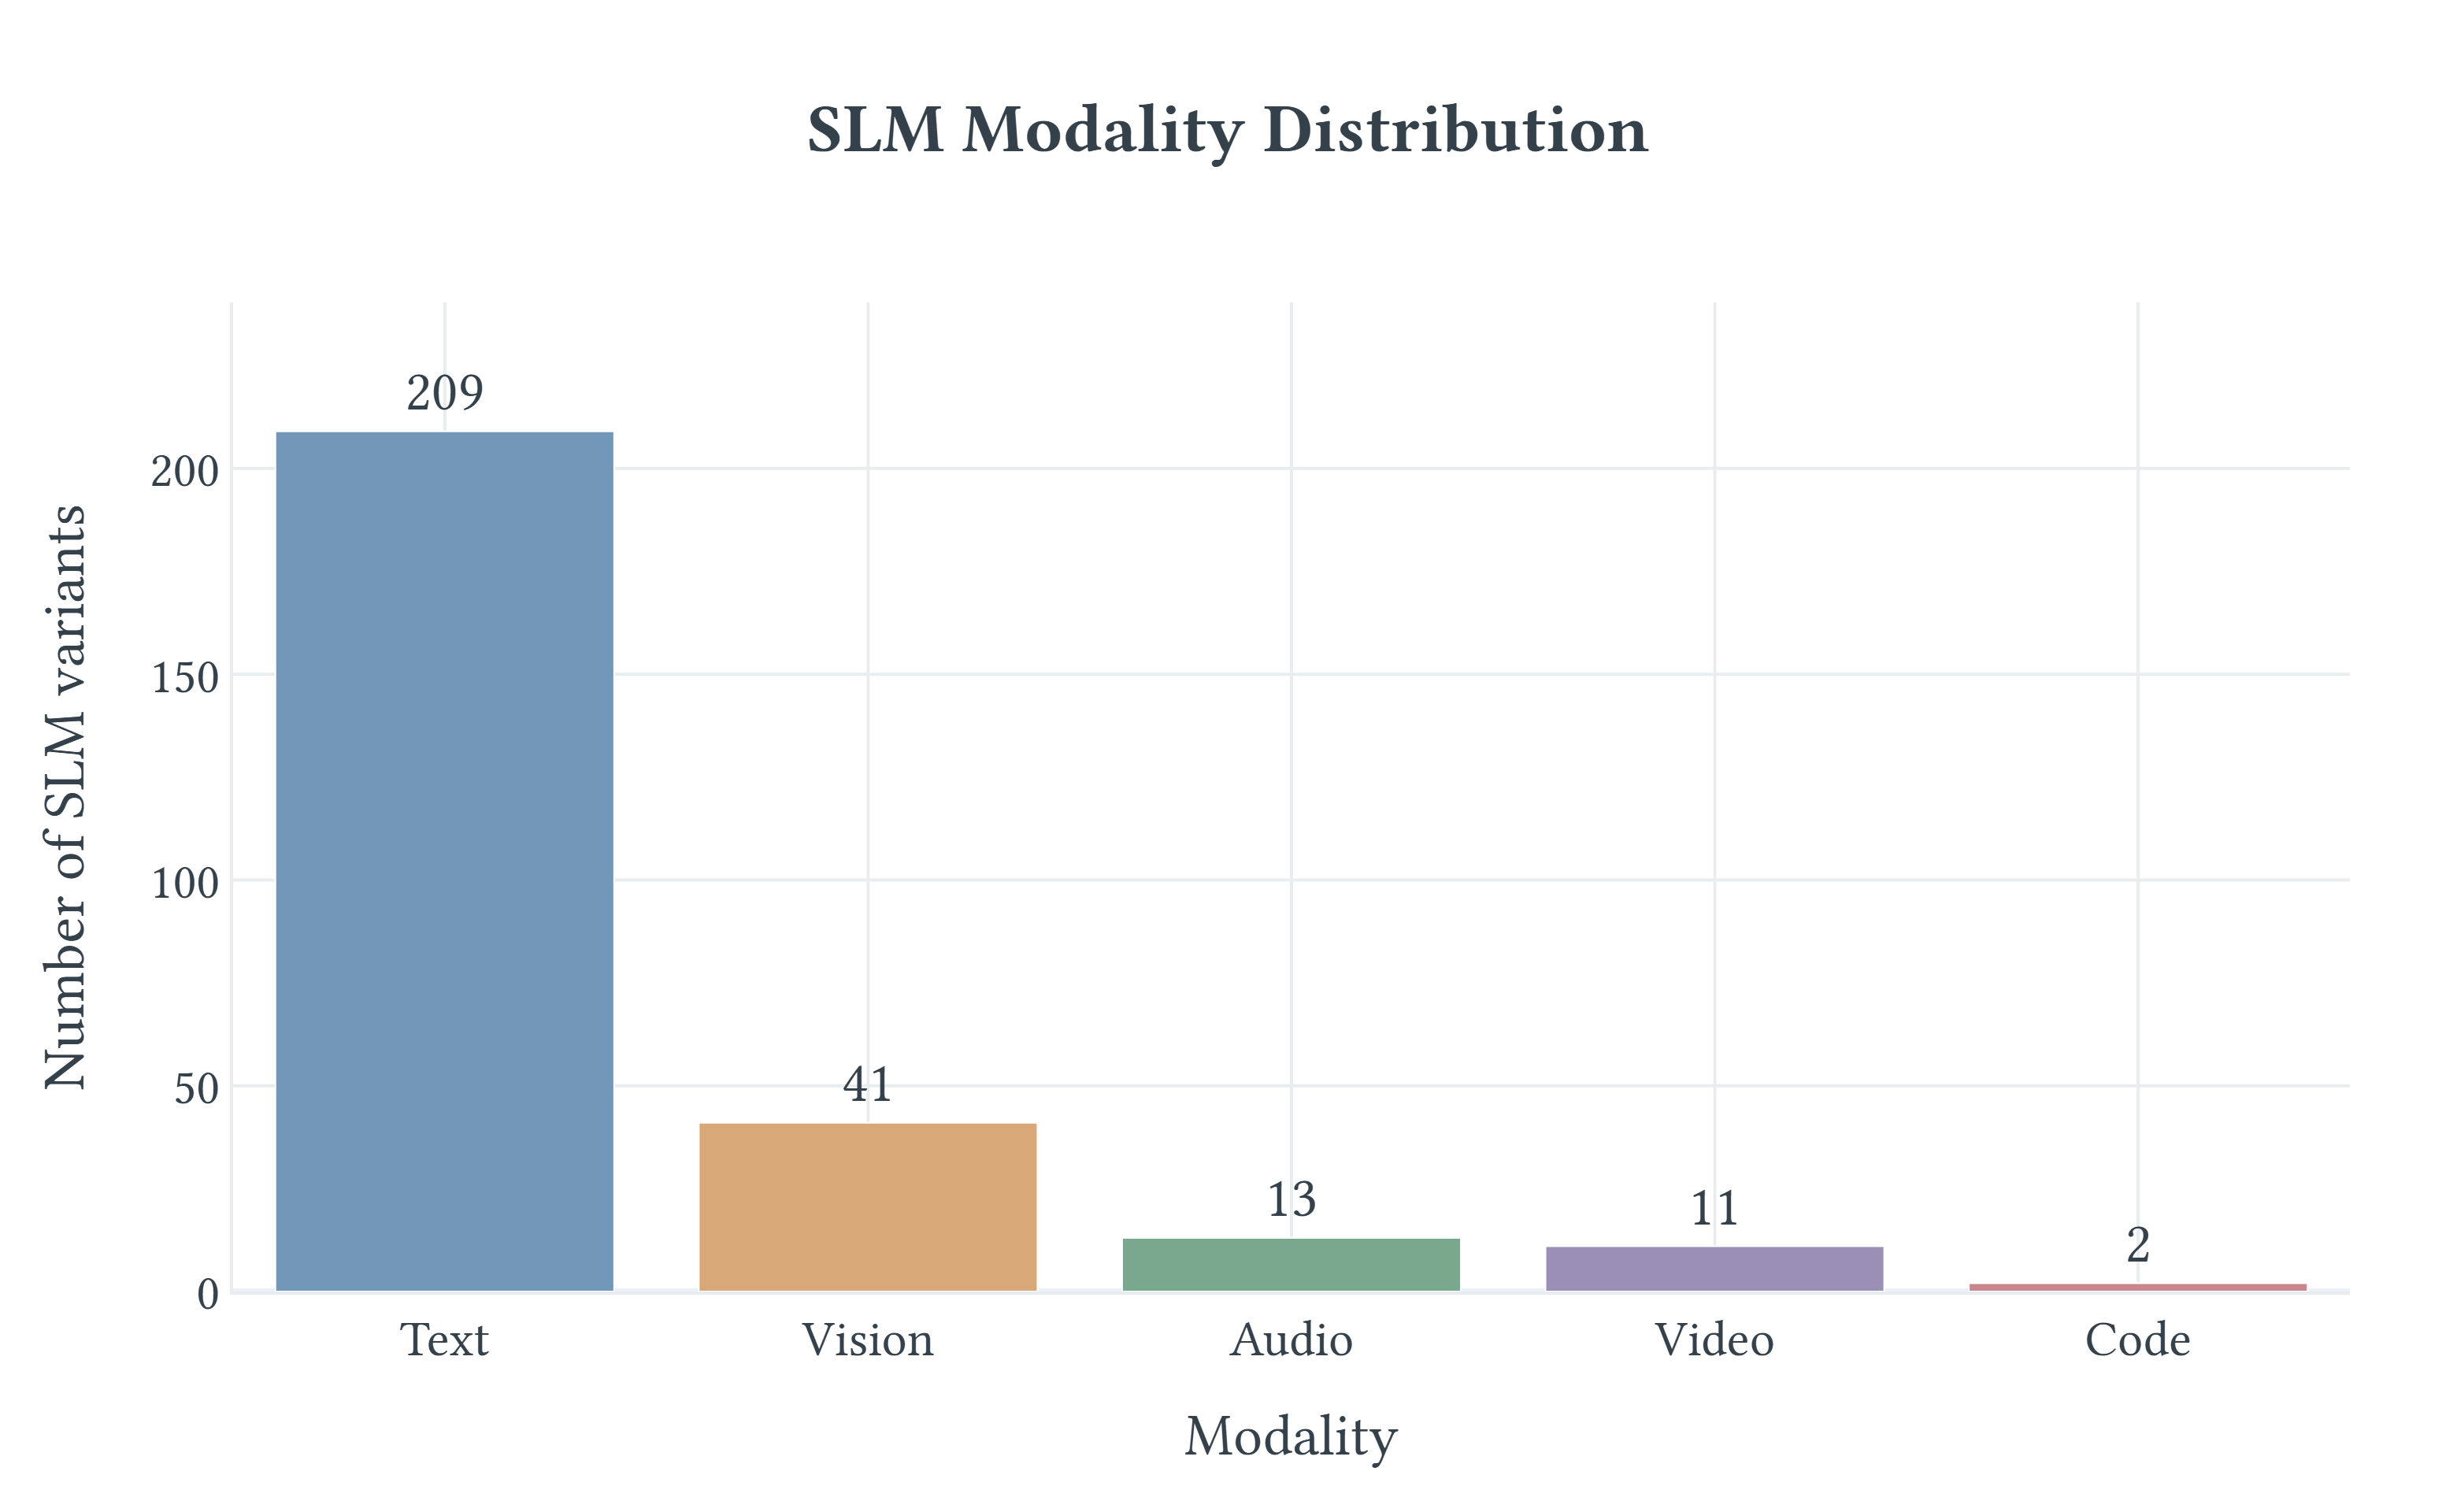
\includegraphics[width=\linewidth]{paper_slm_modality_distribution.png}
  \caption{Input modalities supported by inventory variants (a variant may support several). Text dominates, vision is common, and audio and video remain a small minority.}
  \Description{Bar chart of the number of inventory variants supporting each input modality. Text dominates, vision is common, and audio and video are small categories.}
  \label{fig:modality}
\end{figure}

% Supplementary material: facet detail for Section 3 of the main text.

\section{Taxonomy Facets in Detail}
\label{supp:taxonomy}

This section expands Section~\ref{sec:taxonomy} of the main text.

\subsection{Architecture}
\label{supp:taxonomy_architecture}

\emph{Dense transformers.} Most \glspl{slm} use a dense decoder in which every parameter is active for every token, from SmolLM2-135M \citep{allal2025smollm2} to 7--14B models such as Mistral~7B \citep{jiang2023mistral} and Phi-4. SmolLM3-3B \citep{smollm3} uses grouped-query attention with no positional encoding in a share of its layers and a three-stage curriculum over 11.2T tokens; Qwen3's dense line \citep{qwen3_2025} spans 0.6B--32B with a switch between thinking and non-thinking modes. Three refinements recur. Grouped-query attention \citep{ainslie2023gqa}, adopted by Mistral~7B and most later \glspl{slm}, divides the \gls{kv} cache by the ratio of query to \gls{kv} heads. Long context is reached by raising the rotary base or rescaling positions: Llama~3.2 uses a base of 500{,}000 to reach 128K tokens, Gemma~3 uses 1{,}000{,}000 on its global-attention layers, Phi-4 uses 250{,}000 with a 16K context, and Phi-3-mini's 128K checkpoint uses LongRoPE rescaling. Gated feed-forward layers are standard, SwiGLU in most families and GeGLU in Gemma.

\emph{Mixtures of experts.} \gls{moe} layers \citep{shazeer2017moe,fedus2022switch} activate a subset of expert feed-forward blocks per token through a learned router, so total and active parameters differ. Mixtral~8$\times$7B \citep{jiang2024mixtral} (46.7B total, 12.9B active) is the canonical example; DeepSeek-MoE \citep{dai2024deepseekmoe} uses finer-grained and shared experts (about 2.8B active of 16B); Qwen3-30B-A3B \citep{qwen3_2025} activates 3B of 30B; and Llama~4 Scout \citep{llama4_2025} activates 17B of 109B. All of these are small-active-parameter \glspl{moe} under C1 and C2, while Granite~4.0 Tiny (about 7B total, 1B active) \citep{granite4_2025} is an \gls{slm}. Apple's third-generation on-device model is a 20B-total sparse model that activates 1--4B parameters and keeps its full weights in flash, swapping experts into DRAM on demand \citep{apple2026afm3}; its total count meets C2 at the bound, and its resident memory is set by the swapping policy rather than by the total.

\emph{Hybrid state-space models.} Mamba \citep{gu2023mamba} introduced hardware-aware selective state-space layers that process sequences in linear time. Jamba \citep{lieber2024jamba} interleaves Mamba and attention blocks (one attention layer in eight) and reports a \gls{kv} cache eight times smaller than Mixtral's at 256K context. Falcon-H1 \citep{falconh1_2025} spans 0.5B--34B with parallel Mamba-2 and attention blocks; IBM's Granite~4.0 \citep{granite4_2025} interleaves Mamba-2 and attention at roughly 9:1 with a fine-grained \gls{moe} and reports over 70\% memory reduction for long-context and multi-session inference relative to transformer-only models (\evC); NVIDIA's Nemotron Nano~2 \citep{nvidia2025nemotron_nano2} replaces most attention layers with Mamba-2 in a 9--12B model and reports up to $6\times$ the throughput of Qwen3-8B on long reasoning traces (\evC); and the Qwen3.5 small series uses Gated DeltaNet layers with one full-attention layer in four \citep{qwen3_5_2026}. Linear-time layers matter most where \glspl{slm} are deployed: long, streaming, memory-bound contexts on edge hardware.

\subsection{Training Strategy}
\label{supp:taxonomy_training}

\emph{Trained from scratch.} Phi showed that ``textbook-quality'' synthetic and curated data yields large gains at fixed size \citep{gunasekar2023phi1,li2023phi2}: Phi-1 (1.3B) was trained on under 8B tokens yet reached competitive Python results. Gemma~3 \citep{team2025gemma3} scales its token budget with size, from 2T tokens for the 1B variant to 14T for the 27B, under a curriculum that increases the share of mathematics, code, and multilingual data. Recurring practices are classifier-based quality filtering, synthetic data from larger teachers \citep{tinystories2023,mukherjee2023orca}, curricula that move toward harder data late in training, and continued pre-training for long context.

\emph{Distilled.} Distillation \citep{hinton2015distilling} transfers capability from a teacher, through its internal representations (white-box) or its outputs and generated text (black-box). Orca \citep{mukherjee2023orca} distilled GPT-4 explanation traces into a 13B student. The DeepSeek-R1 distillations \citep{deepseek2025r1} fine-tune Qwen2.5 and Llama students from 1.5B to 70B on long chain-of-thought traces from DeepSeek-R1, and Phi-4-mini-reasoning \citep{xu2025phi4mini_reasoning} combines distillation from a reasoning teacher with reinforcement learning at 3.8B. Gemma~3 and Gemma~4 \citep{team2025gemma3,gemma4_2026} distill every size from a larger teacher.

\emph{Pruned and distilled.} NVIDIA's Minitron pipeline \citep{minitron2024} prunes Nemotron-4 15B in depth and width, guided by activation-based importance, and retrains the pruned 8B and 4B students by distillation from the unpruned model, needing up to $40\times$ fewer training tokens per derived model than training from scratch (a $1.8\times$ compute saving for the family); a follow-up applies the recipe to Llama~3.1 8B and Mistral NeMo 12B \citep{sreenivas2024llmpruning}. Meta derived Llama~3.2 1B and 3B by pruning Llama~3.1 8B and distilling from the 8B and 70B models \citep{meta2024llama32}.

\subsection{Modality}
\label{supp:taxonomy_modality}

\emph{Text-only.} Most families ship text-only variants, and text-only models dominate the inventory (Figure~\ref{fig:modality}).

\emph{Vision--language.} PaliGemma (3B) \citep{beyer2024paligemma} combines a SigLIP image encoder with a Gemma decoder and reports strong transfer after fine-tuning. Phi-3-vision (4.2B) \citep{abdin2024phi3} adds an image encoder to Phi-3-mini for document and chart understanding. Gemma~3 \citep{team2025gemma3} attaches a SigLIP-based encoder, operating on $896 \times 896$ inputs with Pan-and-Scan cropping, to its 4B, 12B, and 27B variants; the 1B variant is text-only with a 32K context. Qwen2.5-VL \citep{bai2025qwen25vl} at 3B and 7B supports documents, charts, and video.

\emph{Audio and multimodal.} Gemma~3n \citep{google2025gemma3n} nests a 2B-effective sub-model inside a 4B-effective one (MatFormer) and keeps per-layer embeddings off the accelerator, so that its 5B and 8B raw models run with the resident memory of roughly 2B and 4B models. Gemma~4 \citep{gemma4_2026} spans 2.3B-effective to 31B with dense and \gls{moe} variants and a thinking mode. Voxtral Mini~3B (4.7B including its audio encoder) adds speech understanding and transcription to a 3B decoder under an open licence \citep{mistral2025voxtral}, and Apple's on-device models are multimodal \citep{gunter2025afm,apple2026afm3}.

\subsection{Application Domains}
\label{supp:taxonomy_domain}

Most \glspl{slm} are general-purpose models evaluated on broad benchmarks. Developer-trained domain models target narrow tasks:

\begin{description}
  \item[Healthcare] Meerkat-7B \citep{kim2025meerkat}, fine-tuned on chain-of-thought traces synthesized from medical textbooks, reports 70.6\% on MedQA, which its authors describe as the first 7B result above the roughly 60\% USMLE pass threshold (\evC). OptimCLM \citep{hasan2024optimclm} compresses clinical BERT encoders with under 5\% macro-AUROC loss on outcome prediction (\evC).
  \item[Code] Code Llama \citep{roziere2023codellama}, StarCoder2 \citep{lozhkov2024starcoder2}, and DeepSeek-Coder \citep{zhu2024deepseek_coder} are code-specialized families evaluated on HumanEval and MBPP (\suppsec~\ref{subsec:applications_code}).
  \item[Legal] Small models fine-tuned on statutes, case law, and contracts target clause classification, obligation extraction, and regulatory triage. On-premises deployment can help meet privilege and data-residency obligations, subject to the scope conditions of Section~\ref{subsec:deployment_privacy_scope}; public evaluation of current small models in this domain is sparse (\suppsec~\ref{subsec:applications_legal}).
  \item[Multilingual] Aya~23 \citep{aryabumi2024aya23} allocates the capacity of an 8B decoder to 23 languages and reports outperforming the 13B Aya-101 \citep{ustun2024aya} on the languages both cover (\evC); Aya-101 is an mT5-based encoder-decoder, outside C1. Qwen2.5-7B \citep{qwen2024qwen25} documents coverage of Chinese, Japanese, Korean, Arabic, and the major European languages.
\end{description}

% Supplementary material: method-level detail for Section 4 of the main text.

\section{Compression Methods in Detail}
\label{supp:compression}

This section expands the summary of Section~\ref{sec:compression} of the main text.

\subsection{Post-Training Quantization}

Post-training quantization needs only a small calibration set (typically 128--512 samples) and no gradient computation, which is why it is the dominant paradigm. GPTQ \citep{frantar2023gptq} quantizes layer by layer, using an approximation of the inverse Hessian of the layer-wise reconstruction loss to choose rounding decisions. \gls{awq} \citep{lin2024awq} observes that about 1\% of weights, those on large-magnitude activation channels, account for a disproportionate share of the quantization error, and applies per-channel scaling to protect them; its authors report higher accuracy than GPTQ at matched bit-width. At 8 bits the obstacle is activations rather than weights: LLM.int8() \citep{dettmers2022llmint8} keeps outlier dimensions in 16-bit, and SmoothQuant \citep{xiao2023smoothquant} migrates the difficulty from activations to weights to enable W8A8 integer kernels; both report accuracy essentially unchanged from FP16. SqueezeLLM \citep{kim2024squeezellm} uses sensitivity-based non-uniform quantization with a dense-and-sparse decomposition. \gls{gguf} \citep{gerganov2023llamacpp} packages weights, vocabulary, and metadata in one file, with block-wise ``K-quant'' schemes from Q2\_K to Q8\_0; mixed schemes such as Q4\_K\_M keep the most sensitive tensors at higher precision.

Two independent benchmarks bear on small models specifically. ThinkSLM \citep{srivastava2025thinkslm} evaluates 72 small models, including quantized and pruned derivatives, on 17 reasoning benchmarks with three repeats, and finds that quantization preserves reasoning ability while pruning disrupts it. SLMQuant \citep{slmquant2025} evaluates quantization methods on two sub-1B models (SmolLM-135M and Qwen2.5-0.5B) on knowledge, commonsense, and language-modeling tasks, and finds that methods tuned on large models transfer imperfectly and that sensitivity depends on architecture: under W4A8 quantization the larger of its two models scored lower than the smaller, which the authors attribute to architectural differences rather than size. Neither study establishes that 4-bit loss grows monotonically as model size falls, and we make no such claim.

\subsection{Quantization-Aware and Low-Bit Training}

Quantization-aware training simulates quantization in the training loop so that weights become robust to it. It recovers part of the accuracy that post-training quantization loses at 2--3 bits, with the margin widening as bit-width falls, but needs training data and compute, which is why it appears mainly in vendor pipelines such as Apple's 2-bit on-device quantization \citep{gunter2025afm}. Its limit case is training in the low-bit format from the start: BitNet b1.58 \citep{ma2024bitnet158} restricts weights to $\{-1,0,1\}$, and the released 2B4T model was trained in that format on four trillion tokens.

\subsection{Pruning}

SparseGPT \citep{frantar2023sparsegpt} extends the GPTQ machinery to weight removal and prunes OPT-175B and BLOOM-176B to 50--60\% unstructured sparsity in one shot with a negligible increase in perplexity. Wanda \citep{sun2024wanda} removes the weights with the smallest product of magnitude and input-activation norm, with no weight update, and its authors report parity with SparseGPT on LLaMA and Llama~2; that parity does not hold below 4B \citep{kurz2025pruning_vs_quant}. Structured pruning removes heads, channels, or layers and yields models that run on dense kernels: LLM-Pruner \citep{ma2023llmpruner} removes coupled structures selected by gradient information and recovers quality with a short \gls{lora} tuning; ShortGPT \citep{men2024shortgpt} deletes the layers that change their input least, and we found no study establishing how far this tolerance holds below 7B (\evD). Sheared-LLaMA \citep{xia2024sheared} prunes Llama~2 7B to 1.3B and 2.7B and reports outperforming same-size open models at about 3\% of the compute of training them from scratch (\evC).

% Supplementary material: knowledge-distillation detail moved from Section 4.2 of the main text.

\section{Knowledge Distillation Variants}
\label{supp:kd}

\subsection{White-Box vs.\ Black-Box KD}

The survey by \citet{yang2024kd_survey} classifies \gls{llm} distillation into two paradigms:

\emph{White-box \gls{kd}} has access to the teacher's intermediate representations. TinyBERT \citep{jiao2020tinybert} pioneered layer-by-layer feature alignment, matching student hidden states, attention matrices, and embedding layers to teacher counterparts via MSE loss. In the decoder-only \gls{llm} setting, this requires pairing student and teacher layers, which is non-trivial when sizes differ substantially, and is computationally expensive but yields superior retention of teacher capabilities.

\emph{Black-box \gls{kd}} uses only the teacher's generated outputs, either token probabilities or free-form text, as the supervision signal. Orca \citep{mukherjee2023orca} exemplifies text-output black-box \gls{kd}: GPT-4 generates explanation traces and step-by-step reasoning, which a 13B LLaMA-based student learns to imitate. DeepSeek-R1 \citep{deepseek2025r1} extends this to long chain-of-thought reasoning distillation, fine-tuning 1.5B--70B Qwen and Llama students on the reasoning traces of its large model trained by reinforcement learning; its authors report that the reasoning patterns of the large model can be transferred to smaller ones in this way (\evC).

\subsection{Chain-of-Thought Distillation}

A particularly productive form of black-box \gls{kd} is \gls{cot} distillation \citep{wei2022cot}: the teacher model generates explicit reasoning steps, and the student learns to produce or internalize these steps. \citet{feng2024counterfactual} demonstrate counterfactual distillation, which augments \gls{cot} traces with contrastive incorrect reasoning, as a way to sharpen the student's reasoning boundaries. \citet{liao2024nesycd} propose Neural-Symbolic Collaborative Distillation, using a neuro-symbolic teacher to provide structured reasoning supervision that is more transferable to small students than purely neural \gls{cot}.

\subsection{Data Augmentation in KD}

The survey by \citet{xu2024kd_survey} highlights data augmentation (DA) as a central paradigm within \gls{kd} frameworks. When the student lacks sufficient coverage of the teacher's knowledge space, the teacher can generate synthetic training instances targeting specific skill gaps, the mechanism underlying the Phi family's success \citep{gunasekar2023phi1}. \citet{ballout2024efficient_kd} use a roughly 3B teacher's most influential input tokens, identified by attribution methods such as saliency maps, as rationales for the student, and report improvements over standard fine-tuning and over prior distillation methods on four datasets.

\subsection{Self-Distillation}

An emerging approach eliminates the external teacher entirely. \citet{fu2024dynamic_selfd} propose Dynamic Self-Distillation, in which the model uses its own predictions from previous mini-batches as soft targets during fine-tuning, providing a form of implicit regularization that reduces overfitting on small fine-tuning datasets, a critical challenge for \glspl{slm}.

% ----------------------------------------------------------------

% Supplementary material: audit protocol detail moved from Section 5.1 of the main text.

\section{Audit Protocol Detail}
\label{supp:audit}

This section expands the protocol summary of Section~\ref{subsec:reported_protocol} of the main text.

\subsection{Benchmark Tasks and Metrics}
\label{subsec:reported_benchmarks}
The benchmarks that recur across the reviewed release documents span seven
capability areas: \gls{mmlu} \citep{hendrycks2021mmlu} for broad knowledge;
ARC-Easy and ARC-Challenge \citep{clark2018arc} and HellaSwag
\citep{zellers2019hellaswag} for commonsense and language reasoning; \gls{gsm8k}
\citep{cobbe2021gsm8k} and MATH \citep{hendrycks2021math} for mathematical
reasoning; HumanEval \citep{chen2021humaneval} and MBPP \citep{austin2021mbpp}
for code generation; TriviaQA \citep{joshi2017triviaqa} and SQuAD~2.0
\citep{rajpurkar2018squad2} for question answering; MNLI \citep{williams2018mnli}
for natural language inference; and SST-2 \citep{socher2013sst} for sentiment
classification. Each benchmark carries a standard metric: accuracy for multiple
choice, exact match or F1 for question answering, pass@1 for code, exact match
for \gls{gsm8k}, and symbolic equivalence for MATH. Instruction-following
(MT-Bench-style \citep{zheng2023mtbench}) and summarization are reported too
sparsely and too heterogeneously to compare at all, and the conventions behind
them are described in \suppsec~\ref{subsec:appendix_human_eval}. Section~\ref{subsec:reported_agentic_gap}
takes up separately the question of whether any of these benchmarks bears on
agentic suitability.

Five conditions determine what a benchmark number means, and a source that omits
any of them has not reported a comparable result. \emph{Benchmark version:}
\gls{mmlu} exists in the original and in MMLU-Pro, ARC in Easy and Challenge
splits, GSM8K in original and GSM8K-Platinum revisions, and HumanEval in the
original and HumanEval+ forms, and these are not interchangeable.
\emph{Prompt template:} whether the model's own chat template is applied,
whether options are lettered or restated, and whether a system prompt is present.
\emph{Answer extraction:} whether a multiple-choice answer is scored by
comparing per-option log-likelihoods or by parsing a generated letter, which can
differ by several points on the same model and benchmark, and for
chain-of-thought tasks, which span of the generation is taken as the answer.
\emph{Decoding settings:} greedy versus sampled, temperature, and for pass@$k$
the number of samples. \emph{Harness:} the framework and its version, most often
\texttt{lm-evaluation-harness} \citep{gao2023harness} or HELM
\citep{liang2023helm}, each with its own defaults for all of the above.

The coverage of these five conditions across the reviewed sources is what
Section~\ref{subsec:reported_overall} reports on, and it is poor. Which
benchmarks a vendor reports, in which version, under how many shots, and with
which extraction rule varies enough to prevent a common table.

\subsection{Coverage Ledger}
\label{subsec:audit_ledger}

Table~\ref{tab:audit_ledger} reproduces the coverage ledger summarized in
Section~\ref{subsec:reported_overall}. Its scope is the instruction-tuned
checkpoints of the 14 cohort models from Microsoft, Alibaba, Meta, and Google,
against the eight benchmarks that recur in their headline reporting; the other
four cohort models (TinyLlama, SmolLM2, StableLM~2, Mistral~7B), each from a
different developer, were not transcribed.
Each cell was transcribed from the model's primary release document or official
model card, listed with its table in the released CSV. Only coverage and stated
protocol are recorded, not scores. Of the 112 cells, 69 carry an
instruction-tuned value and 45 of those state a protocol; no benchmark is reported
for all 14 models; and the largest group of models sharing one stated protocol on
any benchmark is five (\gls{mmlu} at 5 shots; \gls{gsm8k} at 8 shots with
chain-of-thought). Of the reconciliation rules written before collection, rule~(a)
(exclude a value that cannot be cross-checked against a second source) would
exclude nearly every vendor cell by construction, so the finding is stated without
it: protocol mismatch alone (rule~(b)) and separate pre-trained and
instruction-tuned tabulation (rule~(c)) are sufficient to prevent a common table.

% Generated by source/scripts/build_audit_ledger.py; do not edit by hand.
\begin{table}[t]
\centering
\caption{Coverage ledger for the instruction-tuned checkpoints of the 14 cohort models from the four largest vendors: the protocol under which each model's primary release document reports each benchmark. Numbers are shot counts; ``c'' marks chain-of-thought; ``SE'' OpenAI simple-evals defaults; ``u'' a value reported without a stated protocol; ``--'' not reported. Sources and locations are listed in \file{audit\_coverage\_ledger.csv}; transcribed on 8~October 2026.}
\label{tab:audit_ledger}
\footnotesize
\begin{tabular}{lcccccccc}
\toprule
\textbf{Model} & \textbf{MMLU} & \textbf{MMLU-Pro} & \textbf{ARC-C} & \textbf{HellaSwag} & \textbf{GSM8K} & \textbf{MATH} & \textbf{HumanEval} & \textbf{MBPP} \\
\midrule
Phi-3-mini & 5 & -- & 10 & 5 & 8c & -- & 0 & 3 \\
Phi-3.5-mini & 5 & 0c & 10 & 5 & 8c & 0c & 0 & 3 \\
Phi-4-mini & 5 & 0c & 10 & 5 & 8c & 0c & -- & -- \\
Phi-4 & SE & -- & -- & -- & -- & SE & SE & -- \\
Qwen2.5-0.5B & -- & u & -- & -- & u & u & u & u \\
Qwen2.5-1.5B & -- & u & -- & -- & u & u & u & u \\
Qwen2.5-3B & -- & u & -- & -- & u & u & u & u \\
Qwen2.5-7B & -- & u & -- & -- & u & u & u & u \\
Llama 3.2-1B & 5 & -- & 0 & 0 & 8c & 0c & -- & -- \\
Llama 3.2-3B & 5 & -- & 0 & 0 & 8c & 0c & -- & -- \\
Gemma 2-2B & u & -- & -- & -- & -- & -- & -- & u \\
Gemma 2-9B & u & -- & -- & -- & -- & -- & -- & u \\
Gemma 3-1B & 0 & 0 & -- & -- & 0c & 0 & 0 & 3 \\
Gemma 3-4B & 0 & 0 & -- & -- & 0c & 0 & 0 & 3 \\
\midrule
Reported (of 14) & 10 & 8 & 5 & 5 & 11 & 11 & 9 & 10 \\
\bottomrule
\end{tabular}
\end{table}


\subsection{Hardware and Quantization Scope}
\label{subsec:reported_hardware}
The review reads reported behavior against six reference configurations spanning the
cloud-to-edge spectrum (Table~\ref{tab:hardware_configs}) and three precisions:
FP16 (reference), INT8, and INT4, with \gls{gguf}~Q4\_K\_M, GPTQ group-128, and \gls{awq}
group-128 treated as distinct INT4 subclasses when the source distinguishes them.
Inference-framework attribution (vLLM \citep{kwon2023vllm}, llama.cpp
\citep{gerganov2023llamacpp}, ONNX Runtime \citep{microsoft2019onnx}, ExecuTorch
\citep{meta2024executorch}, MLC-LLM \citep{mlc2024}) follows the stack used by the
source of each figure; cross-framework comparisons are made only when compared
figures share a framework or are explicitly flagged.

\subsection{Limitations of the Evidence Base}
\label{subsec:reported_limits}
Because the figures are compiled from heterogeneous public sources rather than a
single controlled pipeline, four limitations bound the strength of every
comparison below. \textbf{Prompt-format and harness variation:} different sources
use different templates and answer-extraction heuristics, which can shift reported
accuracy by several points under the same nominal benchmark. \textbf{Self-reporting
bias:} vendor-reported scores are systematically more favorable than third-party
reproductions; where third-party figures exist, comparisons preferentially use
them and flag the divergence. \textbf{Condition-coverage sparsity:} not every
model has reported scores for every task, tier, or precision. Missing values are
never imputed, interpolated, or carried across from a sibling model size or from
a base checkpoint to its instruction-tuned variant; a tuple with no qualifying
source is recorded as absent, and absence is itself reported, since the pattern
of what vendors decline to publish is part of the finding of
Section~\ref{subsec:reported_overall}. No statistic in this paper is computed
over a set from which absent tuples were silently dropped. \textbf{Snapshot staleness:} the ecosystem evolves monthly,
and figures reflect the state of public reporting at the collection window. These
limitations motivate the empirical-verification agenda of
Section~\ref{subsec:challenges_verification}.

\subsection{Quantization Impact}
\label{subsec:reported_quantization}

The reported picture for the sub-10B regime is summarized in
Table~\ref{tab:compression_quality} of the main text. INT8 post-training
quantization is reported as effectively lossless by the authors of the main
methods \citep{dettmers2022llmint8,xiao2023smoothquant} (\evC). At 4 bits, an
independent benchmark of 72 small models finds reasoning largely preserved
\citep{srivastava2025thinkslm}, and an independent benchmark of two sub-1B models
finds that methods tuned on large models transfer imperfectly, with sensitivity
depending on architecture \citep{slmquant2025} (\evB); neither establishes that
the loss grows monotonically as size falls. \gls{awq} is reported to retain more
accuracy than GPTQ at matched bit-width \citep{lin2024awq} (\evC), and mixed
schemes such as \gls{gguf} Q4\_K\_M keep the most sensitive tensors at higher
precision \citep{gerganov2023llamacpp}. In the controlled comparisons at
0.5--3.8B, post-training quantization preserved fidelity better than
post-training pruning \citep{kurz2025pruning_vs_quant,srivastava2025thinkslm}
(\evA); Section~\ref{subsec:compression_quantization} gives the scope.

Per-model, per-benchmark degradation figures are not reported consistently
enough across this cohort to tabulate: sources differ in harness, calibration
set, and group size, and few publish a matched FP16 baseline alongside the
quantized result. Measuring them under a single toolchain is one of the
verification studies proposed in
Section~\ref{subsec:challenges_verification}.

The memory consequence, by contrast, is firmly established, because it follows
from the storage format rather than from measurement.
Table~\ref{tab:memory_footprint} gives weight footprints estimated from
parameter count and effective bits per weight. The FP16 column is exactly two
bytes per parameter. The four-bit columns correspond to 4.4--5.8 effective bits
per parameter: four-bit weights plus per-group scales and zero-points, with the
embedding and output layers typically kept at higher precision, which is a
larger share of a smaller model. The reduction therefore falls short of the
nominal 4$\times$, at 2.8 to 3.6$\times$ across the table, and is smallest for
the smallest models. Qwen2.5-7B drops from 15.2~GB to 4.2--4.5~GB, and Phi-4-mini
(3.8B) from 7.6~GB to 2.2--2.4~GB, which is what moves each of them across
a hardware tier boundary. The exact figure for a given artifact is its file
size, which should be read from the artifact rather than from this table.

\begin{table}[ht]
\centering
\caption{Model-weight memory footprint by precision (GB). FP16 is two bytes per parameter; the four-bit columns are estimates at 4.4--5.8 effective bits per parameter, including the group scales and higher-precision tensors each scheme retains, which is why the reduction ($2.8$--$3.6\times$) is below the nominal 4$\times$. Activation and KV-cache memory are additional and depend on context length and batch size.}
\label{tab:memory_footprint}
\footnotesize
\begin{tabular}{lcccc}
\toprule
\textbf{Model} & \textbf{FP16} & \textbf{GPTQ-4bit} & \textbf{AWQ-4bit} & \textbf{Q4\_K\_M} \\
\midrule
Qwen2.5-7B & 15.2 & 4.2 & 4.4 & 4.5 \\
Phi-4-mini & 7.6 & 2.2 & 2.3 & 2.4 \\
Llama 3.2-3B & 6.4 & 1.9 & 2.0 & 2.1 \\
SmolLM2-1.7B & 3.4 & 1.1 & 1.1 & 1.2 \\
TinyLlama-1.1B & 2.2 & 0.7 & 0.8 & 0.8 \\
\bottomrule
\end{tabular}
\end{table}


% Supplementary material: reference tables moved from Sections 5 and 6 of the main text.

\section{Cohort and Hardware Reference Tables}
\label{supp:tables}

Table~\ref{tab:model_specs} gives the architectural specifications of the 18-model cohort of Section~\ref{sec:reported}; Tables~\ref{tab:hardware_configs} and~\ref{tab:appendix_hardware} give the reference hardware of Sections~\ref{sec:reported} and~\ref{sec:deployment}.

\begin{table}[ht]
\centering
\caption{Architectural specifications of reviewed models (as reported by each model's official release materials).}
\label{tab:model_specs}
\footnotesize\adjustbox{max width=\linewidth}{%
\begin{tabular}{lccccccc}
\toprule
\textbf{Model} & \textbf{Params} & \textbf{Layers} & \textbf{Hidden} & \textbf{Attention} & \textbf{Context} & \textbf{Vocab} & \textbf{Train Tokens} \\
\midrule
TinyLlama-1.1B & 1.1B & 22 & 2,048 & GQA-32/4 & 2K & 32K & 3.0T \\
SmolLM2-1.7B & 1.7B & 24 & 2,048 & MHA-32h & 8K & 49K & 11.0T \\
StableLM 2-1.6B & 1.6B & 24 & 2,048 & MHA-32h & 4K & 100K & 2.0T \\
Qwen2.5-0.5B & 0.5B & 24 & 896 & GQA-14/2 & 32K & 152K & 18.0T \\
Qwen2.5-1.5B & 1.5B & 28 & 1,536 & GQA-12/2 & 32K & 152K & 18.0T \\
Qwen2.5-3B & 3.0B & 36 & 2,048 & GQA-16/2 & 32K & 152K & 18.0T \\
Qwen2.5-7B & 7.6B & 28 & 3,584 & GQA-28/4 & 128K & 152K & 18.0T \\
Llama 3.2-1B & 1.2B & 16 & 2,048 & GQA-32/8 & 128K & 128K & 9.0T \\
Llama 3.2-3B & 3.2B & 28 & 3,072 & GQA-24/8 & 128K & 128K & 9.0T \\
Gemma 2-2B & 2.6B & 26 & 2,304 & GQA-8/4 & 8K & 256K & 2.0T \\
Gemma 2-9B & 9.2B & 42 & 3,584 & GQA-16/8 & 8K & 256K & 8.0T \\
Gemma 3-1B & 1.0B & 26 & 1,152 & GQA-4/1, LG & 32K & 262K & 2.0T \\
Gemma 3-4B & 4.3B & 34 & 2,560 & GQA-LG & 128K & 262K & 4.0T \\
Mistral 7B & 7.3B & 32 & 4,096 & GQA-32/8 & 8K & 32K & n/a \\
Phi-3-mini & 3.8B & 32 & 3,072 & MHA-32h & 128K & 32K & 3.3T \\
Phi-3.5-mini & 3.8B & 32 & 3,072 & MHA-32h & 128K & 32K & 3.4T \\
Phi-4-mini & 3.8B & 32 & 3,072 & GQA-24/8 & 128K & 200K & 5.0T \\
Phi-4 & 14.0B & 40 & 5,120 & GQA & 16K & 100K & $\sim$10T \\
\bottomrule
\end{tabular}%
}\par\vskip 4pt\relax
{\raggedright \small \textit{Note:} MHA = Multi-Head Attention; \gls{gqa} = Grouped-Query Attention (Q/KV heads); GQA-LG = \gls{gqa} with local--global interleaving. Every model in this cohort is dense, so total and active parameters coincide and a single parameter column suffices; no small-active-parameter \gls{moe} model (Section~\ref{subsubsec:intro_def_terms}) is in the cohort, because none has public reporting complete enough to include.

\textit{On training-token counts.} These are the least reliable column in the
table, and their status differs by row. Marked \emph{per-variant} where the
source states a figure for that specific size: Gemma~2-2B (2.0T), Gemma~2-9B
(8.0T), Gemma~3-1B (2.0T), Gemma~3-4B (4.0T), Phi-3-mini (3.3T), Phi-3.5-mini
(3.4T), Phi-4-mini (5.0T), TinyLlama (3.0T), SmolLM2-1.7B (11.0T), StableLM~2
(2.0T). Marked \emph{series-level} where the source reports one figure for the
whole family and the individual sizes are not separately stated: Qwen2.5
(18.0T across 0.5B--7B) and Llama~3.2 (9.0T across 1B and 3B). Phi-4's
${\sim}10$T is an approximation given as such by its source. Mistral~7B's
training-token count is not disclosed. We report series-level figures in the
size rows they cover rather than omitting them, but they should not be read as
independent per-model measurements, and no claim in this paper relies on
comparing a series-level figure against a per-variant one.

\textit{On context length.} The value is the maximum the primary source
documents, which for several models is reached through position interpolation at
inference rather than trained natively: Qwen2.5-7B is natively 32K and extended
to 128K, and Phi-3-mini's 128K is a separate long-context checkpoint from the 4K
base.\par}
\end{table}

\begin{table}[ht]
\centering
\caption{Reference hardware configurations used to organize the deployment discussion of Section~\ref{sec:deployment}. They define the tiers against which reported figures are read; no per-model, per-configuration result is tabulated, because the sources do not report one consistently (Section~\ref{subsec:deployment_calc_vs_meas}).}
\label{tab:hardware_configs}
\footnotesize\adjustbox{max width=\linewidth}{%
\begin{tabular}{lllll}
\toprule
\textbf{Configuration} & \textbf{Hardware} & \textbf{RAM/VRAM} & \textbf{TDP} & \textbf{Use Case} \\
\midrule
Cloud GPU & NVIDIA A100 80GB & 80 GB HBM2e & 300W & Training + serving \\
High-end Consumer & NVIDIA RTX 4090 & 24 GB GDDR6X & 450W & Local inference \\
CPU/iGPU Laptop & AMD Ryzen 7 7840HS & 32 GB DDR5 & 35--54W & Laptop deployment \\
Edge GPU Module & NVIDIA Jetson Orin Nano & 8 GB LPDDR5 & 7--15W (25W Super) & Edge AI / robotics \\
Edge SBC & Raspberry Pi 5 & 8 GB LPDDR4X & 12W & Embedded IoT \\
Mobile SoC & Snapdragon 8 Gen 3 & 12 GB LPDDR5X & $\sim$8W sustained & Smartphone \\
\bottomrule
\end{tabular}%
}
\end{table}

\begin{table}[ht]
\centering
\caption{Detailed specifications of the devices referenced in this section.}
\label{tab:appendix_hardware}
\footnotesize\adjustbox{max width=\linewidth}{%
\begin{tabular}{lcccc}
\toprule
\textbf{Specification} & \textbf{Raspberry Pi 5} & \textbf{Jetson Orin Nano} & \textbf{Galaxy S24+} & \textbf{Laptop} \\
\midrule
CPU & BCM2712 4$\times$A76 @ 2.4GHz & 6$\times$A78AE @ 1.5GHz & Snapdragon 8 Gen 3 & Ryzen 7 7840HS \\
GPU & VideoCore VII & 1024 CUDA (Ampere) & Adreno 750 & Radeon 780M \\
NPU & None & None & Hexagon & Ryzen AI \\
RAM & 8 GB LPDDR4X & 8 GB LPDDR5 (unified) & 12 GB LPDDR5X & 32 GB DDR5-5600 \\
Memory bandwidth & $\sim$17 GB/s & 68 GB/s & 76.8 GB/s & 89.6 GB/s \\
Storage & microSD / NVMe & NVMe & UFS 4.0 & NVMe SSD \\
TDP & 12W & 7--15W (25W Super) & $\sim$8W sustained & 35--54W \\
Inference engine & llama.cpp & MLC LLM & ExecuTorch & llama.cpp \\
\bottomrule
\end{tabular}%
}
\end{table}

Table~\ref{tab:taxonomy_summary} summarizes the four primary facets of the taxonomy of Section~\ref{sec:taxonomy} with representative models.

\begin{table}[ht]
\centering
\caption{Summary of the four primary facets of the SLM taxonomy with representative models. Assignment is multi-label: a model may carry several categories on one facet, and the same model may therefore appear more than once in a block.}
\label{tab:taxonomy_summary}
\footnotesize\adjustbox{max width=\linewidth}{%
\begin{tabular}{llll}
\toprule
\textbf{Facet} & \textbf{Category} & \textbf{Key Characteristics} & \textbf{Representative Models} \\
\midrule
\multirow{3}{*}{Architecture}
 & Dense Transformer & All params active per token; GQA, RoPE, SwiGLU & Phi-4-mini, Qwen3, SmolLM3, Gemma 3 \\
 & MoE              & Sparse activation; total $\gg$ active params       & Granite 4.0 Tiny (SLM); Mixtral 8$\times$7B, Qwen3-30B-A3B (small-active MoE) \\
 & Hybrid SSM-Transformer & Linear-time; interleaved SSM/attention blocks   & Falcon-H1, Granite 4.0, Nemotron Nano 2 \\
\midrule
\multirow{3}{*}{Training Strategy}
 & From scratch     & Curated/synthetic data; full pre-training          & Phi, Qwen2.5/Qwen3, SmolLM3 \\
 & Distillation     & Knowledge transfer from larger teacher             & Gemma 3/4, DeepSeek-R1-Distill, Phi-4-mini-reasoning \\
 & Pruning-based    & Parameter removal from large model + distillation  & Minitron, Sheared-LLaMA \\
\midrule
\multirow{3}{*}{Modality}
 & Text-only        & Tokenized text I/O; majority of production SLMs   & Mistral 7B, SmolLM3, Qwen3 \\
 & Vision-Language  & Image + text; CLIP/SigLIP encoder added            & Phi-3-vision, Gemma 3 (4B and above), PaliGemma \\
 & Audio/Multimodal & Text + vision + audio in one sub-10B model         & Gemma 3n, Gemma 4, Apple AFM \\
\midrule
\multirow{4}{*}{Domain}
 & General-purpose  & Multi-domain training; evaluated on broad benchmarks & Phi, Gemma, Llama, Qwen, Mistral \\
 & Healthcare       & Clinical NLP; on-premises for data residency        & Meerkat 7B, OptimCLM \\
 & Code             & Code corpora; FIM training; HumanEval/MBPP focus  & Code Llama, StarCoder2, DeepSeek-Coder \\
 & Legal/Multilingual & Domain corpora; regulatory and cross-lingual tasks & Aya 23 8B, Qwen2.5 multilingual \\
\bottomrule
\end{tabular}%
}
\end{table}

Table~\ref{tab:deployment_frameworks} compares the deployment frameworks of Section~\ref{subsec:deployment_frameworks}.

\begin{table}[ht]
\caption{Key SLM deployment frameworks, their primary targets, and characteristics. Throughput is not tabulated, because project-reported figures are measured on different hardware and settings and are not comparable across rows (Section~\ref{subsec:deployment_calc_vs_meas}).}
\label{tab:deployment_frameworks}
\centering
\footnotesize\adjustbox{max width=\linewidth}{%
\begin{tabular}{@{}lllp{5.5cm}@{}}
\toprule
\textbf{Framework} & \textbf{Primary Target} & \textbf{Quantization} & \textbf{Notes} \\
\midrule
llama.cpp \citep{gerganov2023llamacpp}   & CPU, Metal, CUDA, ROCm & GGUF (Q2--Q8)   & Widely used reference runtime; minimal dependencies; ecosystem includes Ollama, llamafile \\
ONNX Runtime \citep{microsoft2019onnx} & GPU, CPU, NPU, WASM & INT4/INT8       & Cross-platform; DirectML, CoreML, CUDA backends \\
MLX \citep{mlx2023}             & Apple Silicon          & 4-bit           & Unified memory; no host--device weight transfers \\
TensorRT-LLM \citep{nvidia_tensorrt2024} & NVIDIA GPUs   & INT4/INT8/FP16  & Continuous batching; kernel fusion \\
ExecuTorch \citep{meta2024executorch} & Mobile (iOS, Android) & INT4          & Small base runtime; CoreML, QNN, ARM, MediaTek, Vulkan backends; used for Meta's Llama~3.2 on-device measurements \\
MLC-LLM \citep{mlc2024}        & iOS, Android, web, embedded GPU & 4-bit          & TVM compilation; WebGPU support \\
WebLLM \citep{webllm2024}       & Web browsers           & 4-bit WASM     & WebGPU acceleration; OpenAI-compatible API \\
\bottomrule
\end{tabular}%
}
\end{table}

Table~\ref{tab:taxonomy_facets} gives the secondary facets of the taxonomy.

\begin{table}[t]
\centering
\caption{Secondary facets. These do not describe what a model is but whether it can be adopted, and they are the facets practitioners report finding hardest to recover from model cards. Access and license are recorded per variant in the released inventory, though for 96 of the 209 records the license is given only as a pointer to the source; the other facets are assigned in this paper to representative models.}
\label{tab:taxonomy_facets}
\footnotesize\adjustbox{max width=\linewidth}{%
\begin{tabular}{@{}lp{5.4cm}p{4.6cm}@{}}
\toprule
\textbf{Facet} & \textbf{Values} & \textbf{Why it gates adoption} \\
\midrule
Licensing & Permissive (Apache-2.0, MIT); custom vendor licence with use restrictions; research-only; unspecified; proprietary/API-only & Determines commercial use, redistribution of fine-tunes, and whether an on-premises deployment is legal at all \\
Data transparency & Full (corpus released); partial (composition described, data not released); disclosed sources only; undisclosed & Determines whether contamination, licensing of training data, and domain fit can be assessed \\
Safety alignment & Preference-optimized with a published safety evaluation; instruction-tuned without one; base model only & A base checkpoint wired into an agent with tool access has no refusal behavior to rely on \\
Reasoning mode & None; always-on extended reasoning; controllable budget; separate reasoning checkpoint & Determines token cost per call and whether latency is predictable, which is decisive inside an agent loop \\
Deployment target & Documented inference engine(s) and hardware class the vendor ships an artifact for & An unquantized checkpoint with no GGUF, ONNX, or ExecuTorch export is not an edge model whatever its size \\
\bottomrule
\end{tabular}%
}
\end{table}

% Supplementary material: moved from Sections 6.1-6.2 of the main text.

\section{Platforms and Device Tiers in Detail}
\label{supp:deployment}

\subsection{Apple Intelligence (AFM)}

Apple's Foundation Models \citep{apple2024intelligence,gunter2025afm} are the most fully documented on-device \gls{slm} deployment. The 2025 report \citep{gunter2025afm} describes a $\sim$3B on-device model, optimized for Apple silicon through KV-cache sharing (dividing the model so the second block reuses the first block's cache, a reported 37.5\% memory saving) and 2-bit quantization-aware training, paired with a Parallel-Track Mixture-of-Experts server model on Private Cloud Compute. The on-device model is reported competitive with Qwen3-4B and Gemma-3-4B on its target tasks, and the server model with Llama~4 Scout (\evC). The third-generation family \citep{apple2026afm3}, five models built in collaboration with Google, adds a 20B-total on-device model that activates 1--4B parameters per token and keeps its full weights in flash, swapping experts into DRAM as needed; Private Cloud Compute was extended to NVIDIA GPUs in Google Cloud. This followed a January 2026 joint statement that Apple's next foundation models would be based on Gemini models and cloud technology \citep{google_apple2026statement}. Google's Gemini Nano, the on-device member of the Gemini family \citep{gemini2023}, occupies the same design point on Android.

\subsection{Samsung Gauss}

Samsung announced Gauss in November 2023 as a family of generative models in three parts, Gauss Language, Gauss Code, and Gauss Image, used first for internal productivity and planned for its products \citep{samsung2023gauss}. Samsung has published no parameter count, architecture, or on-device specification for it, so Gauss fails criterion M1, is not in the inventory, and we make no claim about its deployment. It is listed here because it is frequently cited as an on-device \gls{slm}, and the published record does not support that description.

\subsection{General Mobile Deployment Considerations}

\glspl{slm} targeting mobile deployment must navigate three constraints. (1) \emph{Memory}: Consumer smartphones typically provide 6--12~GB RAM, of which the OS uses 2--4~GB, leaving 4--8~GB for applications. A 3B model at Q4 requires ${\sim}2$~GB, comfortable for most flagship devices. (2)~\emph{Thermal}: Sustained inference on mobile \glspl{npu} is throttled by thermals; realistic sustained throughput is lower than peak throughput benchmarks suggest. (3)~\emph{Battery}: published per-device battery figures are scarce and not reported under a common protocol. The fundamental constraint in edge decoding is memory bandwidth rather than compute: flagship phones and mainstream laptops offer on the order of 50--100~GB/s (single-board computers well under 30~GB/s, unified-memory laptop designs considerably more) versus 2--3~TB/s for datacenter GPUs \citep{xu2024device}, making INT4 quantization not merely a storage optimization but a performance enabler for single-stream generation.

% ----------------------------------------------------------------
\subsection{Edge and IoT Deployment}
\label{subsec:deployment_edge}

Below smartphone-class hardware lies a diverse ecosystem of edge devices: Raspberry Pi single-board computers, NVIDIA Jetson modules, and microcontrollers. \glspl{slm} targeting this tier typically require:

\begin{description}
    \item[Sub-1B or extreme quantization] A Raspberry Pi~5 (8~GB RAM, Cortex-A76 CPU, about 17~GB/s of memory bandwidth) can hold 4-bit models up to a few billion parameters, and its decode rate is bounded by that bandwidth. A benchmark of runtimes on single-board computers reports that llamafile reaches up to $4\times$ the throughput of Ollama at 30--40\% lower power for equivalent models \citep{nguyen2025sbc} (\evB).

    \item[Jetson Orin] NVIDIA's Jetson Orin modules, with TensorRT-LLM \citep{nvidia_tensorrt2024} among their runtimes, hold quantized 3--7B models in 8--64~GB of unified memory, with the larger-memory NX and AGX parts suited to the upper end of that range, for industrial and robotics use.

    \item[Microcontrollers (MCU)] ARM Cortex-M class microcontrollers carry roughly 512~KB--2~MB of SRAM. Even a 10M-parameter model needs about 5~MB at 4 bits, and a 100M-parameter one about 50~MB, so a language model of the size this survey covers cannot be resident in microcontroller SRAM, and would at best stream weights from external memory at a large cost in speed. Keyword detection and sensor analytics on these parts are served by task-specific networks far smaller than any model in the inventory; we found no documented \gls{slm} deployment at this tier, and it is outside the scope of this paper.
\end{description}

Table~\ref{tab:appendix_hardware} details the specifications of the four
representative devices referenced throughout this section, from the Raspberry~Pi
5 up to a laptop-class CPU.

% ----------------------------------------------------------------

% Supplementary material: moved from Sections 7.6 and 7.7 of the main text.

\section{Conversion Pipeline and Barriers to Adoption}
\label{supp:agentic}

\subsection{Converting an LLM Agent to an SLM Agent}
\label{subsec:agentic_conversion}

For teams with an existing LLM-only agent, \citet{belcak2025slm_agentic} propose a six-step conversion pipeline, which we summarize here because it operationalizes the position; the steps are theirs. \textbf{S1, instrumentation:} log every non-interface model call (inputs, outputs, latency) from the running agent, with encryption and access control. \textbf{S2, curation:} strip personally identifiable and protected health information and application secrets from the logs. \textbf{S3, clustering:} apply unsupervised clustering to the curated calls to surface the recurring request types, which are the specialization targets. \textbf{S4, selection:} for each cluster, choose a candidate \gls{slm} by matching required capability against benchmarks, license, and deployment constraints. \textbf{S5, specialization:} fine-tune the chosen \gls{slm} on the cluster's curated data, typically with \gls{lora} or \gls{qlora}. \textbf{S6, iteration:} re-run the loop periodically as the traffic distribution drifts. Two additions follow from H. Step~S3 is where the conditions are assessed: each cluster's output schema (H1), input length (H3), and the availability of validity and correctness checks (H4a, H4b) can be checked by inspection, and its volume can be compared with a pilot estimate of the break-even $N^{*}$ (H2), recorded before the comparison; clusters that fail are left with the generalist. And each converted cluster should be evaluated on cost per completed task against the unconverted agent, which is the measurement the literature lacks.

\subsection{Barriers to Adoption}
\label{subsec:agentic_barriers}

\citet{belcak2025slm_agentic} identify three reasons the shift has lagged the technical case. First, large centralized-inference investments create sunk-cost inertia and an operational bias toward one big model behind one API (B1). Second, \glspl{slm} are still evaluated on generalist leaderboards (\gls{mmlu}, broad chat benchmarks) that are misaligned with agentic utility, so their fitness for delegated sub-tasks is under-measured (B2). Section~\ref{sec:reported} shows that the generalist record is also too inconsistent across vendors to support cross-model comparison, so it cannot be used to choose among small models even for general capability. Third, \gls{slm} releases receive far less attention than frontier launches, so awareness lags capability (B3). The first and third are not technical obstacles. The second is different, and Section~\ref{subsec:agentic_evidence} shows it to be partly a real evidential gap rather than only a misdirected emphasis: agent-specific evaluation exists and is maturing \citep{patil2025bfcl,yao2024taubench,barres2025tau2,liu2024agentbench,kapoor2025hal}, and developer reports support per-call competence for specialized small models, but independent multi-step evaluations of current sub-10B models are sparse, and no study compares cost per completed task for small-model-first and large-model agents. Until that changes, the strength of the case for hypothesis~H will remain uneven in the way Table~\ref{tab:agentic_evidence} records.

\subsection{Learned Routing and Cascades}
\label{subsubsec:agentic_routing}

Three designs recur. \emph{Cascades} try the cheap model first and escalate on a quality signal: FrugalGPT \citep{chen2023frugalgpt} learns which sequence of \gls{llm} APIs to query, and AutoMix \citep{aggarwal2024automix} escalates when the small model's own few-shot self-verification judges its answer unreliable, which is the pattern H prescribes when the checker of H4 is the model itself. \emph{Predictive routers} decide before generation: Hybrid~LLM \citep{ding2024hybridllm} routes by predicted query difficulty with a quality level tunable at test time, and RouteLLM \citep{ong2024routellm} trains a lightweight router on human-preference data to predict whether a weak model's answer would be judged as good as a strong model's, reporting transfer of the trained router to unseen strong/weak model pairs. \emph{Decomposing routers} push the decision below the query level: Division-of-Thoughts \citep{division_of_thoughts_2025} decomposes a task into sub-questions and assigns each to a local \gls{slm} or a cloud \gls{llm} according to estimated difficulty, for on-device agents. The open problems are difficulty estimation without an oracle, routing objectives that jointly weigh accuracy, latency, privacy sensitivity, and network availability, and handoff that does not produce a visible seam in output quality \citep{demystifying2025slm}.

A different form of SLM--LLM collaboration leaves the large model in charge of every output and uses the small one only to make it faster. In speculative decoding a small draft model proposes several tokens and the large model verifies them in one forward pass, accepting a prefix, so that the output distribution is that of the large model \citep{leviathan2023speculative,chen2023specsampling}; Medusa \citep{cai2024medusa} and EAGLE \citep{li2024eagle} replace the separate draft model with lightweight heads on the large model itself. This is not delegation in the sense of H, since no call's answer comes from the small model, but it is the most widely deployed way in which small models already reduce the cost of large-model inference, and it is complementary to routing: an escalated call can itself be served speculatively.


% Supplementary material: moved from Section 8 of the main text.

\section{Domain-Specific Applications in Detail}
\label{supp:applications}

This section expands the summary of Section~\ref{sec:applications} of the main text.

\subsection{Healthcare and Clinical NLP}
\label{subsec:applications_healthcare}

Healthcare \gls{nlp} presents demanding requirements: high factual accuracy, interpretability, compatibility with clinical workflows, and operation within a regulatory regime that constrains where identifiable patient data may be processed. That regime is the pull toward on-premises models, and it needs stating precisely, because it is frequently overstated.

\emph{On-premises deployment is not compliance.} Neither HIPAA nor the GDPR is
satisfied by the location of a model's weights. HIPAA compliance is a property of
a covered entity's administrative, physical, and technical safeguards taken
together: access control, audit logging, integrity controls, transmission
security, workforce training, breach notification, and business-associate
agreements where a third party is involved. The GDPR requires a lawful basis for
processing, purpose limitation, data minimization, a data protection impact
assessment for high-risk processing, and, for automated decisions with legal or
similarly significant effects, the safeguards of Article~22. A locally hosted
model can fail every one of these. What on-premises deployment does is remove one
specific difficulty, the transfer of identifiable data to a processor outside the
entity's control, which under HIPAA otherwise requires a business-associate
agreement and under the GDPR raises transfer and sub-processor questions. That is
a real and often decisive simplification, and it is the reason the pull exists.
It is not a compliance property of the model, and no claim in this paper should
be read as asserting one. The same scope conditions as
Section~\ref{subsec:deployment_privacy_scope} apply: an on-premises model whose
application logs prompts to a cloud service has reintroduced the transfer it was
chosen to avoid.

The Meerkat family \citep{kim2025meerkat} demonstrates the potential of domain-specific \gls{slm} fine-tuning. Built on a 7B base with instruction fine-tuning on curated clinical QA data and chain-of-thought traces synthesized from medical textbooks, Meerkat-7B reports 70.6\% on MedQA (USMLE-style), which its authors describe as the first 7B result above the USMLE passing threshold, ahead of earlier open medical models and GPT-3.5 across six medical benchmarks though below GPT-4 (\evC). The larger Meerkat-70B is reported to exceed GPT-4 by 1.3 points on average and to diagnose 21 of 38 complex clinical cases, against 21.8 for GPT-4 and 13.8 for human respondents (\evC). Meerkat-7B runs on a single GPU; Meerkat-70B needs about 140~GB at 16-bit precision.

OptimCLM \citep{hasan2024optimclm} distils an ensemble of domain-adapted clinical BERT encoders into the smaller BERT-PKD and TinyBERT, then applies unstructured pruning and 8-bit quantization, reporting up to $22.88\times$ compression with under 5\% loss in macro-AUROC on length-of-stay, mortality, diagnosis, and procedure prediction from MIMIC-III admission notes. It shows that the compression stages compose for clinical classifiers that can run on hospital workstations; it is not evidence about generative \glspl{slm}.

The broader \gls{slm} healthcare ecosystem includes domain-pretrained biomedical models in the 2--3B range, clinical note generation models, and radiology-specific models. A key trend is the use of \gls{rag} \citep{lewis2020rag} to anchor \gls{slm} outputs to verified clinical knowledge bases, reducing hallucination rates in patient-facing applications.

\subsubsection{The State of the Evidence in This Domain}
\label{subsubsec:applications_health_evidence}

Healthcare is the best-evidenced of the verticals surveyed here, and it is still
weaker evidence than it appears. Three qualifications apply to everything above.

\emph{Licensing-exam benchmarks are not deployment evidence.} MedQA and its
siblings are multiple-choice examinations designed to test candidate physicians,
and performance on them establishes that a model can answer exam questions. It
does not establish accuracy on the tasks clinical systems actually perform:
coding an encounter, drafting a discharge summary, extracting a medication list
from a note, or flagging a contraindication. The Meerkat results are
grade-\evC{}, author-reported on public benchmarks with a documented method,
which is a good standard for the model literature and not the standard a clinical
deployment decision requires.

\emph{Independent prospective evaluation is largely absent.} We found no
prospective study evaluating a sub-10B model in a live clinical workflow with
outcome measurement, and no head-to-head comparison of an on-premises small model
against a cloud frontier model on the same institution's data under the same
protocol. Retrospective benchmark performance and deployment performance are
known to diverge in clinical \gls{nlp}, and nothing in the current \gls{slm}
literature closes that gap.

\emph{Compression results are single-study.} The OptimCLM finding
\citep{hasan2024optimclm} that compressed clinical encoders lose under 5\% in
macro-AUROC on outcome prediction is one pipeline, on one dataset, for
classification rather than generation. It has not been independently reproduced,
and no comparable study exists for a compressed generative \gls{slm} on clinical
tasks such as coding an encounter or drafting a discharge summary.

The honest summary is that healthcare provides the strongest published case for
domain-specific small models and that the case rests on exam benchmarks and
single studies rather than on deployment evidence. Establishing per-task clinical
benchmarks with independent evaluation, and reporting per-group performance
floors of the kind Section~\ref{subsec:challenges_ethics} argues for, is an open
need in this vertical specifically.

\subsection{Legal NLP}
\label{subsec:applications_legal}

Legal document processing, which covers contract review, compliance monitoring, regulatory change analysis, and case law search, involves long and precisely structured documents where hallucination is particularly dangerous. \glspl{slm} address legal \gls{nlp} deployment constraints in two ways: (1)~by enabling on-premises deployment to satisfy attorney-client privilege and data security requirements; and (2)~by enabling cost-effective processing of the massive volumes of routine legal work that would be prohibitively expensive with frontier \glspl{llm}.

The argument for domain-adapted \glspl{slm} (3B--7B, fine-tuned on contract corpora) in this vertical is structural rather than empirical: contract review, compliance triage, and regulatory monitoring consist of bounded, highly repetitive classification and extraction operations over documents that frequently cannot leave the client's infrastructure, which is precisely the profile the conversion pipeline of Section~\ref{subsec:agentic_conversion} targets. Narrow fine-tuning on a specific regulatory regime concentrates in-domain knowledge that a generalist model must retrieve or infer.

We state the evidential position for this vertical explicitly, because it is
weaker than for the other three and it would be easy to read the structural
argument above as though it were a result. Public legal benchmarks exist: LegalBench
\citep{guha2023legalbench} collects 162 legal-reasoning tasks, LexGLUE
\citep{chalkidis2022lexglue} groups legal language-understanding tasks, and CUAD
\citep{hendrycks2021cuad} provides expert-annotated contract clauses. What is
missing is their use for the current generation of small decoder models: we
found no evaluation of 2024--2026 sub-10B models across them under a common
protocol, and deployment comparisons rest on vendor pilot reports that are not
independently verifiable, often because the corpora are client-confidential. Two structural
features of the domain make this worse: an error in contract or compliance work
can be both consequential and hard to detect, which is exactly the condition
under which hypothesis~H's verifiability requirement (Section~\ref{subsec:intro_thesis})
fails; and long, cross-referential documents strain the short-context condition.
Legal work is therefore a domain where the economic case for small models is
strong and the capability evidence is absent, and we present the section as such
rather than as a claim of parity. Establishing open legal-domain benchmarks with
independent evaluation is a prerequisite for saying anything stronger.

\subsection{Code Generation}
\label{subsec:applications_code}

Code-focused \glspl{slm} have matured into a category distinct from general \glspl{slm}, with specialized pre-training corpora (GitHub, Stack Overflow, documentation), code-aware tokenization, and evaluation on function-level benchmarks (HumanEval, MBPP, SWE-Bench).

\begin{description}
    \item[Code Llama \citep{roziere2023codellama}] Meta's family of code models fine-tuned on Llama 2 (7B, 13B, 34B). Code Llama 7B achieves 33.5\% HumanEval pass@1.

    \item[StarCoder2 \citep{lozhkov2024starcoder2}] BigCode's 3B/7B/15B models trained on The Stack v2 (600+ programming languages). StarCoder2-7B reports 35.4\% HumanEval pass@1, and StarCoder2-15B 46.3\%.

    \item[DeepSeek-Coder \citep{zhu2024deepseek_coder}] A 1.3B--33B family trained from scratch on 2T tokens. The 6.7B base model reports 49.4\% on Python HumanEval, and its instruction-tuned version 78.6\%, above the 76.2\% the same report gives for GPT-3.5-Turbo.

    \item[Codestral \citep{mistral2024codestral}] Mistral's 22B code model trained on 80+ programming languages with fill-in-the-middle (FIM) training for IDE integration. At 22B dense it is just outside the C1/C2 bound and is not in the inventory; it is listed as the upper reference for this category.
\end{description}

\subsection{Education and Multilingual NLP}
\label{subsec:applications_multilingual}

Multilingual \glspl{slm} address the linguistic coverage gap in AI assistants: the majority of \gls{llm} pre-training data is English, leaving speakers of lower-resource languages with markedly worse performance. Aya~23 \citep{aryabumi2024aya23} allocates the capacity of an 8B decoder to 23 languages and reports outperforming its predecessor Aya-101 \citep{ustun2024aya}, a 13B mT5-based encoder-decoder covering 101 languages (outside C1), on the languages both cover (\evC); the pair illustrates the breadth-versus-depth trade-off at this size. Qwen2.5 \citep{qwen2024qwen25} and Gemma~3 \citep{team2025gemma3} document large non-English pretraining mixtures and report multilingual evaluations (\evC). For educational use, which includes on-device tutoring and low-connectivity tools, the requirements beyond language coverage are low hallucination rates and age-appropriate safety filtering, neither of which is reported comparably across small models.

% Supplementary material: moved from Sections 10.1, 10.2, 10.4 and 10.5 of the main text.

\section{Model-Level Challenges in Detail}
\label{supp:challenges}

\subsection{Hallucination Mitigation in Small Models}
\label{subsec:challenges_hallucination}

Hallucination, the confident generation of factually incorrect content, is an intrinsic failure mode of autoregressive language models, and it is more pronounced in smaller models \citep{zhang2023siren}. The core issue is information capacity: a 3B model's parameters can encode far fewer facts than a 175B model, and when queried about knowledge at the boundary of its training distribution, small models are more likely to confabulate plausible-sounding but incorrect responses.

Mitigation strategies include: (1)~\emph{\gls{rag}} \citep{lewis2020rag}, which anchors \gls{slm} generation to retrieved documents rather than parametric memory; (2)~\emph{uncertainty quantification} through sampling and ensemble methods; (3)~\emph{RLHF with truthfulness rewards} to penalize confident incorrect responses; and (4)~\emph{calibration post-processing} to align model confidence to actual accuracy.

\subsection{Reasoning Limitations Under Parameter Constraints}
\label{subsec:challenges_reasoning}

Language-modeling loss falls as a power law in parameter count \citep{kaplan2020scaling}, and in the reported results reviewed here the gap between small and large models is widest on multi-step reasoning, particularly in mathematics, formal logic, and scientific inference (\evD). At the 1B--7B scale, \glspl{slm} struggle with problems that require holding many intermediate states simultaneously or with deep deductive chains.

Emerging directions include: (1)~\emph{Test-time scaling}: allocating additional inference compute (more generation tokens, repeated sampling, tree-of-thought search) to substitute for model capacity; the DeepSeek-R1 authors \citep{deepseek2025r1} report that distilling the long chains of thought of their large reasoning model into 1.5B--70B students transfers much of its mathematical-reasoning ability (\evC). (2)~\emph{Neuro-symbolic integration}: augmenting \glspl{slm} with symbolic solvers (SAT solvers, theorem provers, calculators) to handle formal reasoning externally. (3)~\emph{Speculative decoding} \citep{leviathan2023speculative,chen2023specsampling} using a small draft \gls{slm} to propose tokens verified by a larger model, which speeds up the larger model rather than substituting for it (Section~\ref{subsubsec:agentic_routing}).

\subsection{Hardware Co-Design and NPU Optimization}
\label{subsec:challenges_hardware}

The efficiency of \gls{slm} inference depends as much on hardware as on model architecture. Modern consumer hardware increasingly includes dedicated AI accelerators: Apple ANE, Qualcomm Hexagon \gls{npu} \citep{qualcomm2024ondevice}, Samsung Exynos \gls{npu}, and Intel \gls{npu}. These accelerators are optimized for specific operation types (INT4/INT8 matrix multiplication) and data layouts.

A critical open problem is \emph{hardware-model co-design}: developing \gls{slm} architectures whose attention patterns, FFN widths, and layer counts align with the data bus widths and tile sizes of target \glspl{npu}. Future \glspl{slm} trained with hardware constraints as first-class objectives, rather than retrofitting quantization after the fact, will likely yield significant efficiency improvements.

\subsection{Ethical Considerations: Bias Amplification in Compressed Models}
\label{subsec:challenges_ethics}

Model compression introduces an underexplored ethical risk: \emph{bias amplification}. Pruning and quantization may disproportionately affect model performance on underrepresented demographic groups, dialects, and languages, as the model's remaining capacity may preferentially serve the majority distributions present in training data \citep{blodgett2020language}. \citet{kurz2025pruning_vs_quant} find that quantization preserves multilingual perplexity better than pruning, suggesting that pruning disproportionately degrades non-English performance.

Research priorities include: (1)~\emph{fairness-aware compression} that includes demographic parity metrics as part of the compression objective; (2)~\emph{representation auditing} of compressed models across language, dialect, gender, and race; and (3)~\emph{minimum performance floors} for safety-critical applications, ensuring compressed models meet baseline accuracy thresholds for all user populations.

\subsection{Sustainable AI: SLMs as a Green AI Alternative}
\label{subsec:challenges_sustainability}

The energy consumption of training and serving frontier \glspl{llm} has become a significant environmental and economic concern \citep{strubell2019energy,patterson2022carbon}. Training GPT-3 emitted an estimated 552 metric tons of CO$_2$ equivalent \citep{patterson2021carbon}, and training a model two orders of magnitude smaller from scratch needs correspondingly less compute. The defensible claim about inference is conditional: \emph{for a task a small model completes correctly, on hardware it keeps busy, serving it with the small model uses less inference energy} (\evD). Whether a shift to small models reduces total system energy depends on teacher-training energy, the compression pipeline, device embodied carbon, regional grid intensity, update distribution, utilization, and the rebound effect, and no published accounting answers it. \suppsec~\ref{supp:energy} sets out the accounting boundary.

\subsection{Democratization and Sustainability}
\label{supp:democratization}

Running a 3B model with strong reported grade-school-mathematics accuracy on an
inexpensive single-board computer is a qualitative change in access.
Organizations facing cloud-API cost, data-sovereignty rules, or unreliable
connectivity can run capable \gls{nlp} locally with no per-query charge and,
subject to the scope conditions of Section~\ref{subsec:deployment_privacy_scope},
without transferring prompt content to a processor outside their control. The
environmental side of the argument is conditional in the way set out above and in
\suppsec~\ref{subsubsec:challenges_env_scope}: we make a per-task inference claim
and no aggregate one.


% Supplementary material: moved from Section 10.7 of the main text.

\section{Open Research Directions}
\label{supp:directions}

Beyond direct empirical verification, several promising research directions emerge from this review:

\begin{description}
    \item[Multilingual \gls{slm} evaluation] Extending the consolidated performance evidence to non-English benchmarks would reveal whether the English-centric performance hierarchy reported in the literature holds across languages, particularly for models with multilingual training data (Qwen2.5, Gemma~3, BLOOM).

    \item[On-device continual learning] Developing methods for incremental adaptation of deployed \glspl{slm} to new data without full retraining would enable personalization and domain adaptation at the edge.

    \item[SLM ensembles vs.\ single \gls{llm}] Investigating whether ensembles of specialized \glspl{slm} (one for math, one for code, one for general knowledge) with a lightweight router can match single-LLM performance at lower aggregate cost.

    \item[Multimodal \glspl{slm}] Evaluating vision-language \glspl{slm} such as Phi-3-vision, Gemma~3 with vision, and Gemma~3n \citep{google2025gemma3n} on multimodal benchmarks would extend the comparison to the rapidly growing multimodal inference domain.

    \item[Hybrid architectures] The emergence of non-transformer \gls{slm} architectures (SambaY \citep{ren2025sambay}, Gated Delta Networks \citep{yang2025gated_delta}) suggests that the transformer's dominance may not extend to the edge, where linear-time inference is particularly valuable.

    \item[Federated fine-tuning] Developing privacy-preserving fine-tuning protocols that aggregate gradient updates across edge devices would enable collaborative model improvement without centralized data collection.
\end{description}

% Supplementary material: the accounting boundary for environmental claims.

\section{What the Environmental Claim Covers}
\label{subsubsec:challenges_env_scope}
\label{supp:energy}

Environmental claims for small models are routinely made at a level of generality the accounting does not support. A statement that many small-model instances on consumer hardware use less total energy than one multi-GPU server, for example, cannot be sourced or derived: its truth depends on utilization on both sides, and a server at high batch utilization is considerably more energy-efficient per token than a consumer device performing occasional single-stream inference.

A complete comparison of a small-model deployment against a large-model one has to include the training energy of the small model; the training energy of any teacher used to distill it, which can dominate and which vendors do not report; the energy of the distillation, quantization, or pruning pipeline; the embodied carbon of the devices inference runs on, amortized over their service life and the share of it spent on inference; the marginal grid intensity where each side runs, which differs by more than a factor of ten between regions; and the energy of model updates, which for on-device models means redistributing weights to every device.

Almost none of these terms is reported. The available measurements are per-query and partial: a 2023 estimate put a frontier query at about ten times the energy of a web search \citep{devries2023energy}, while a 2025 production measurement covering accelerators, host systems, idle capacity, and data-centre overhead reports 0.24~Wh for the median text prompt of one large assistant \citep{elsworth2025google_energy}. Per-token compute scales with active parameters, so for a query both can answer a small model performs one to two orders of magnitude less compute than a frontier model; whether that becomes an energy saving depends on the utilization of the hardware each runs on (\evD). The defensible claim is therefore conditional: \emph{for a task a small model completes correctly, on hardware it keeps busy, serving it with the small model uses less inference energy}. Whether a shift to small models reduces total system energy is a question no published accounting answers, and the rebound effect, that cheaper inference induces more of it, cuts against it.

\section{Data Provenance and Supplementary Protocols}
\label{appendix:supplementary}
\label{app:provenance}

This appendix supports the reproducibility of the \emph{review itself}: it documents the sources of the reported figures consolidated in Sections~\ref{sec:reported}--\ref{sec:deployment}, and provides the reference prompt templates and quantization-pipeline specifications under which those figures were reported. (The \gls{qlora} adaptation recipe appears in Section~\ref{sec:reported}, Table~\ref{tab:hyperparam_search}; detailed device specifications appear in Section~\ref{sec:deployment}, Table~\ref{tab:appendix_hardware}.) The appendix does not report original experimental runs.

\subsection{Provenance of the Consolidated Figures}
\label{subsec:appendix_provenance_table}

% -----------------------------------------------------------------------------
% AUTHOR ACTION REQUIRED BEFORE SUBMISSION.
% Table \ref{tab:provenance_models} below records model-level provenance, which is
% complete. Per-cell attribution for Tables \ref{tab:finetuning},
% \ref{tab:edge_deployment}, \ref{tab:energy} and \ref{tab:latency_compare} is NOT
% yet reproduced anywhere in this manuscript. Either (a) supply the per-cell
% source ledger for those four tables, or (b) withdraw them and the claims that
% depend on them. Section \ref{subsec:appendix_provenance_status} states the
% current position honestly, but it is not a substitute for (a) or (b).
% -----------------------------------------------------------------------------

Provenance is recorded at two levels. \emph{Model-level} provenance fixes, for
each model in the cohort, the primary release document from which its
architectural specification and headline benchmark scores derive
(Table~\ref{tab:provenance_models}). \emph{Source-class} provenance records, for
each consolidated table, the categories of source the figures are drawn from and
the reconciliation rules applied
(Section~\ref{subsec:appendix_provenance_status}). Benchmark definitions and
metric variants follow the originating task papers cited in
Section~\ref{subsec:reported_benchmarks}.

\begin{table}[ht]
\centering
\caption{Model-level provenance for the reviewed cohort: the primary release document from which each model's architectural specification and headline reported scores derive.}
\label{tab:provenance_models}
\footnotesize\adjustbox{max width=\linewidth}{%
\begin{tabular}{llll}
\toprule
\textbf{Model(s)} & \textbf{Developer} & \textbf{Primary source} & \textbf{Source type} \\
\midrule
TinyLlama-1.1B & --- & \citet{zhang2024tinyllama} & Technical report \\
SmolLM2-1.7B, -360M & Hugging Face & \citet{allal2025smollm2} & Technical report \\
StableLM 2-1.6B & Stability AI & \citet{stabilityai2024stablelm} & Technical report \\
Qwen2.5-0.5B/1.5B/3B/7B & Alibaba & \citet{qwen2024qwen25} & Technical report \\
Llama 3.2-1B/3B & Meta & \citet{grattafiori2024llama3} & Technical report \\
Gemma 2-2B/9B & Google DeepMind & \citet{gemma2team2024} & Technical report \\
Gemma 3-1B/4B & Google DeepMind & \citet{team2025gemma3} & Technical report \\
Mistral 7B & Mistral AI & \citet{jiang2023mistral} & Technical report \\
Phi-3-mini & Microsoft & \citet{abdin2024phi3} & Technical report \\
Phi-3.5-mini & Microsoft & \citet{abdin2024phi35} & Technical report \\
Phi-4-mini & Microsoft & \citet{microsoft2025phi4mini} & Technical report \\
Phi-4 & Microsoft & \citet{abdin2024phi4} & Technical report \\
Ministral 8B & Mistral AI & Vendor model card & Model card \\
\bottomrule
\end{tabular}%
}
\end{table}

\subsection{Provenance Status by Table}
\label{subsec:appendix_provenance_status}

The consolidated tables do not all rest on an equally firm reporting base, and
the distinction matters for how much weight each should carry.

\emph{Architectural and accuracy figures.} The specifications in
Table~\ref{tab:model_specs} and the accuracy figures in
Tables~\ref{tab:zero_shot} and~\ref{tab:appendix_zero_shot_extended} derive from
the primary release documents in Table~\ref{tab:provenance_models}, supplemented
where a model's report omits a task by standardized community evaluations
(the Open \gls{llm} Leaderboard and \texttt{lm-evaluation-harness}-based reports
\citep{gao2023harness}). These are the best-supported figures in the review.

\emph{Compression and quantization figures.} The degradation figures in
Table~\ref{tab:quantization} and the footprints in
Table~\ref{tab:memory_footprint} derive from the quantization-method literature
\citep{frantar2023gptq,lin2024awq,kim2024squeezellm} and from published
quantized artifact sizes. The comparative characteristics in
Table~\ref{tab:compression_compare} are a synthesis of the compression
literature reviewed in Section~\ref{sec:compression} rather than measurements of
a single cohort, and the retention column should be read as an indicative band
rather than a measured quantity.

\emph{Adaptation, efficiency, and energy figures.} Tables~\ref{tab:finetuning},
\ref{tab:edge_deployment}, \ref{tab:energy} and~\ref{tab:latency_compare} rest on
a materially thinner base. Public reporting of fine-tuning gains, edge
throughput, and per-inference energy is sparse, is rarely produced under a common
protocol, and in several cases exists only for a subset of the cohort; some
entries are consequently aggregates or interpolations across sources rather than
single quoted values, and this manuscript does not reproduce a per-cell ledger
for them. They are offered as indicative orders of magnitude that establish
relative position, not as measurements, and no claim in this paper should be
read as resting on their precise values. Converting them into measured
quantities is the first item on the verification agenda of
Section~\ref{subsec:challenges_verification}.

The remaining subsections of this appendix document the reference conditions---prompt formats, quantization toolchains, adaptation hyperparameters---that the reviewed sources most commonly report; these are preserved here so that readers can interpret any individual reported figure against the conditions it was measured under.

\subsection{Prompt Formats}
\label{subsec:appendix_prompt_templates}
The reviewed source materials commonly preserve each model's own instruction
wrapper while following a shared task-payload structure, which is summarized here
in prose. \textbf{Multiple-choice question answering} presents the question
followed by the enumerated options (A--D) and an ``Answer:'' cue, with the model
expected to emit a single option letter. \textbf{Mathematical reasoning} prepends
an instruction to solve the problem step by step and appends a ``Let's think step
by step'' cue, so that a chain-of-thought precedes the final numeric answer.
\textbf{Extractive question answering} supplies the context passage, then the
question, then an instruction to answer from the context and to respond
``unanswerable'' when the context does not contain the answer. \textbf{Abstractive
summarization} supplies the source article preceded by an instruction to produce a
two- to three-sentence summary. Where a source reports few-shot results, the same
fixed set of exemplars is prepended to the payload for every model on a given
task. Because sources differ in the exact wording of these wrappers and in
answer-extraction heuristics, the consolidated figures are compared only within
tasks and, wherever possible, within a single reporting source.

\subsection{Quantization and Compression Pipeline}
\label{subsec:appendix_quantization_pipeline}
To complement the methodology section, the compression workflows reported across the reviewed sources are summarized here. The reviewed literature reports five precision or compression settings across the consolidated comparison:
\begin{description}
    \item[FP16 baseline] Standard half-precision inference used as the reference condition.
    \item[GGUF Q4\_K\_M] Mixed-precision 4-bit quantization via \texttt{llama.cpp}, assigning higher precision to the most sensitive tensors.
    \item[AWQ 4-bit] Activation-aware weight quantization with group size 128 and calibration on held-out text sequences.
    \item[GPTQ 4-bit] Layer-wise post-training quantization using second-order curvature approximations.
    \item[bitsandbytes NF4] 4-bit NormalFloat quantization with double quantization, matching the \gls{qlora} training regime.
\end{description}

For compression stress tests, the sources report SparseGPT~\citep{frantar2023sparsegpt}-induced 50\% unstructured sparsity applied before 4-bit quantization. Reported figures for this combined pruning-plus-quantization setting are retained in the provenance tables for sensitivity analysis rather than the main comparative tables, because support for sparse inference remains hardware dependent and is not uniformly reported across the reviewed sources.

\subsection{Edge Measurement Protocols Reported in the Source Literature}
\label{subsec:appendix_edge_protocol}
The deployment figures consolidated in Sections~\ref{sec:reported}--\ref{sec:deployment} are drawn from source materials whose stated measurement protocols typically include a multi-minute warm-up to stabilize thermal and frequency behavior before measurement. Across the reviewed edge-deployment sources, the reported per-model, per-device measurements cover:
\begin{description}
    \item[Time-to-first-token (\gls{ttft})] Reported latency from prompt submission to first generated token, typically averaged over 50 prompts with 128-token inputs.
    \item[Sustained throughput] Reported mean tokens-per-second over 256-token generations.
    \item[Peak memory] Reported maximum RAM or unified-memory consumption during generation.
    \item[Load time] Reported elapsed time from process start until the model is ready to serve requests.
    \item[Energy per inference] Reported device-level power estimates where the source provides counter- or telemetry-based measurements.
\end{description}
Because these reporting conventions differ in small but potentially consequential ways across sources (warm-up duration, prompt-length distribution, power-counter granularity), readers should treat the consolidated figures as indicative rather than precisely comparable; the conflict-resolution rules in Section~\ref{subsec:reported_sources} are applied whenever discrepant protocols yield materially different reported values for the same tuple.

\subsection{Extended Results Tables}
\label{subsec:appendix_extended_results}
The representative five-shot results for the four models with fine-tuning
comparisons, and the QLoRA hyperparameter configuration used to produce them, are
given with the fine-tuning comparison itself in Section~\ref{sec:reported}
(Table~\ref{tab:finetuning}, Table~\ref{tab:hyperparam_search}) rather than
repeated here.

\begin{landscape}
\begin{table}[ht]
\centering
\caption{Extended zero-shot results across a broader task set (FP16, instruction-tuned variants). All values are reported figures.}
\label{tab:appendix_zero_shot_extended}
\footnotesize\adjustbox{max width=\linewidth}{%
\begin{tabular}{lcccccccccccc}
\toprule
\textbf{Model} & \textbf{ARC-E} & \textbf{ARC-C} & \textbf{HellaSwag} & \textbf{TriviaQA} & \textbf{SQuAD 2.0} & \textbf{GSM8K} & \textbf{MATH} & \textbf{HumanEval} & \textbf{MBPP} & \textbf{MMLU} & \textbf{SST-2} & \textbf{MNLI} \\
\midrule
Phi-4-mini-Inst. & 92.1 & 83.7 & 69.1 & 68.5 & 74.2 & 88.6 & 64.0 & 72.0 & 74.8 & 67.3 & 92.4 & 72.1 \\
Qwen2.5-7B-Inst. & 94.8 & 90.1 & 80.0 & 72.4 & 76.8 & 88.7 & 60.4 & 84.8 & 79.2 & 72.6 & 93.8 & 74.6 \\
Gemma 2-9B-Inst. & 95.2 & 89.8 & 87.1 & 71.8 & 75.5 & 84.9 & 51.3 & 68.9 & 73.5 & 71.3 & 93.5 & 73.8 \\
Gemma 3-4B-Inst. & 92.4 & 85.2 & 78.4 & 64.2 & 70.8 & 82.1 & 53.7 & 64.6 & 69.3 & 65.8 & 91.2 & 70.4 \\
LLaMA 3.2-3B-Inst. & 88.5 & 76.1 & 77.2 & 58.6 & 65.4 & 75.6 & 46.7 & 58.5 & 62.4 & 61.8 & 88.2 & 63.5 \\
LLaMA 3.2-1B-Inst. & 78.2 & 62.3 & 63.8 & 42.5 & 52.8 & 47.2 & 24.1 & 35.4 & 40.2 & 48.6 & 82.5 & 54.2 \\
Mistral 7B-Inst. v0.3 & 91.8 & 82.7 & 73.5 & 65.8 & 68.4 & 81.9 & 41.6 & 66.5 & 68.3 & 63.0 & 90.8 & 68.2 \\
Ministral 8B-Inst. & 93.2 & 85.4 & 76.8 & 67.2 & 71.2 & 83.5 & 45.2 & 69.5 & 71.8 & 65.7 & 92.1 & 71.5 \\
Qwen2.5-3B-Inst. & 90.2 & 78.6 & 72.1 & 58.8 & 66.5 & 79.8 & 50.2 & 65.2 & 67.8 & 65.6 & 89.5 & 66.8 \\
Qwen2.5-0.5B-Inst. & 68.4 & 52.1 & 48.3 & 28.5 & 38.2 & 38.5 & 18.7 & 22.0 & 28.4 & 47.5 & 78.2 & 48.5 \\
SmolLM2-1.7B-Inst. & 74.5 & 59.8 & 60.2 & 35.4 & 52.3 & 42.6 & 19.3 & 28.7 & 35.6 & 50.1 & 82.6 & 54.2 \\
SmolLM2-360M-Inst. & 55.8 & 38.2 & 42.5 & 18.2 & 32.4 & 15.8 & 5.2 & 8.5 & 12.3 & 33.4 & 72.4 & 42.8 \\
TinyLlama 1.1B & 62.4 & 47.5 & 53.8 & 28.8 & 42.5 & 18.4 & 6.8 & 12.2 & 16.8 & 36.2 & 76.5 & 46.2 \\
StableLM 2 1.6B & 72.8 & 55.2 & 57.6 & 32.5 & 48.6 & 32.1 & 12.4 & 22.5 & 28.9 & 44.3 & 80.2 & 52.5 \\
\bottomrule
\end{tabular}%
}
\end{table}
\end{landscape}

\subsection{Human-Evaluation Conventions in the Source Literature}
\label{subsec:appendix_human_eval}
For subjective tasks such as summarization quality and instruction following, the reviewed sources that report human judgments typically rate outputs along three axes---\textbf{relevance}, \textbf{coherence}, and \textbf{factual accuracy}---on a 1--5 Likert scale, with model identity hidden from annotators and inter-annotator reliability reported via a Krippendorff-style coefficient. MT-Bench-style results substitute a strong \gls{llm} judge for human raters. Because these protocols differ across sources in rubric wording and judge model---and because per-model coverage is sparse---instruction-following and summarization are not tabulated in this review and are discussed only qualitatively.

\section{Broader Small-Model Ecosystem Context}
\label{appendix:ecosystem}
\label{supp:last}

This appendix situates the reviewed \gls{slm} cohort within the wider model ecosystem, which matters because the 2025--2026 release cycle moved compact open models, open-weight reasoning models, and frontier API systems in parallel rather than in sequence. The summary below records the ecosystem context needed to interpret the cohort, followed by the full generated variant inventory.

\subsection{Landscape Snapshot}
\label{subsec:ecosystem_snapshot}
Three ecosystem trends are especially relevant to the present study:
\begin{description}
    \item[Capability compression] Reasoning, long-context handling, and multimodality have moved into the 1B--8B range, narrowing the gap between deployable \glspl{slm} and cloud-scale \glspl{llm}.
    \item[Open-weight expansion] Families such as Qwen, Phi, Gemma, SmolLM, DeepSeek distills, Granite, and MiniCPM have expanded the design space for self-hosted deployment (Figure~\ref{fig:license_posture}).
    \item[Deployment diversification] Inference targets now span cloud GPUs, consumer GPUs, laptops, smartphones, browsers, and embedded edge boards, making model choice inseparable from hardware choice.
    \item[The small-active-parameter turn] The most distinctive feature of the mid-2026 wave is how much of it activates 3--13B parameters against totals of 30B to 284B: Nemotron 3.5 Lightning (30B/3B), Hy-MT2-30B-A3B, North Mini Code (30B/3B), Laguna XS 2.1 (33B/3B), Ling 3.0 Flash (124B/5.1B) and its domain variants, and DeepSeek V4 Flash (284B/13B). These are the models that make the C1/C2 distinction load-bearing rather than pedantic, since each is cheap per token and none is resident on a phone.
\end{description}

The May--September 2026 additions to the inventory illustrate both ends of the range. At the small end, IBM shipped Granite 4.1 and then Granite 4.2 at 3B and 8B with a thinking switch, Liquid AI extended LFM2.5 from 230M to an 8.3B/1.5B on-device \gls{moe}, and Tencent released the Hy-MT2 translation family at 1.8B and 7B. Frontier API releases continued in parallel over the same months; they are recorded, with their sources, in the \gls{llm} part of the released inventory, and none of them bears on a claim in this paper.

Figure~\ref{fig:family_treemap} gives a size-proportional overview of the inventory by developer and family, and Figure~\ref{fig:developer_diversity} tracks the entry of new developers into the open-SLM space.

\begin{figure}[ht]
  \centering
  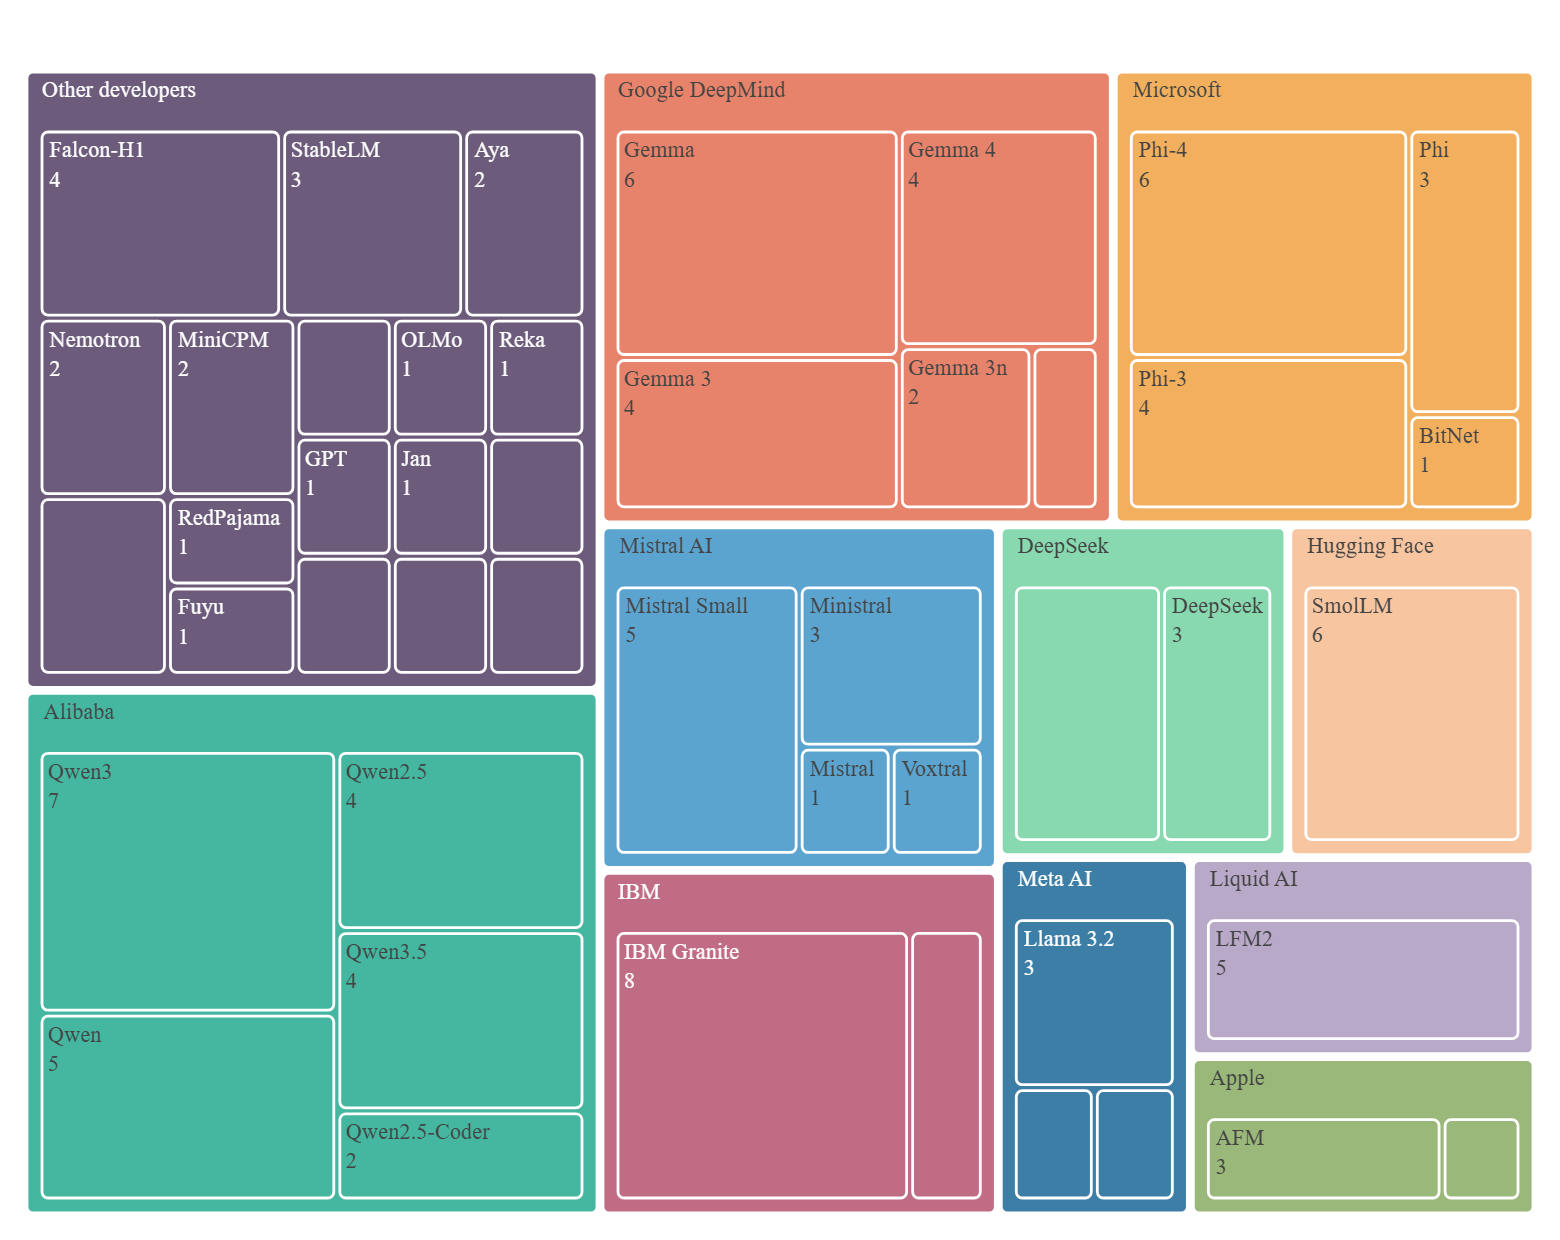
\includegraphics[width=\linewidth]{paper_slm_family_treemap.png}
  \caption{Documented SLM variants grouped by developer and family; area is proportional to the number of variants. Generated from \file{merged\_llm\_database.json} (version~3.6; releases through 4~September 2026).}
  \Description{Treemap of documented small language model variants grouped by developer and then by family, with rectangle area proportional to the number of variants in each group.}
  \label{fig:family_treemap}
\end{figure}

\begin{figure}[ht]
  \centering
  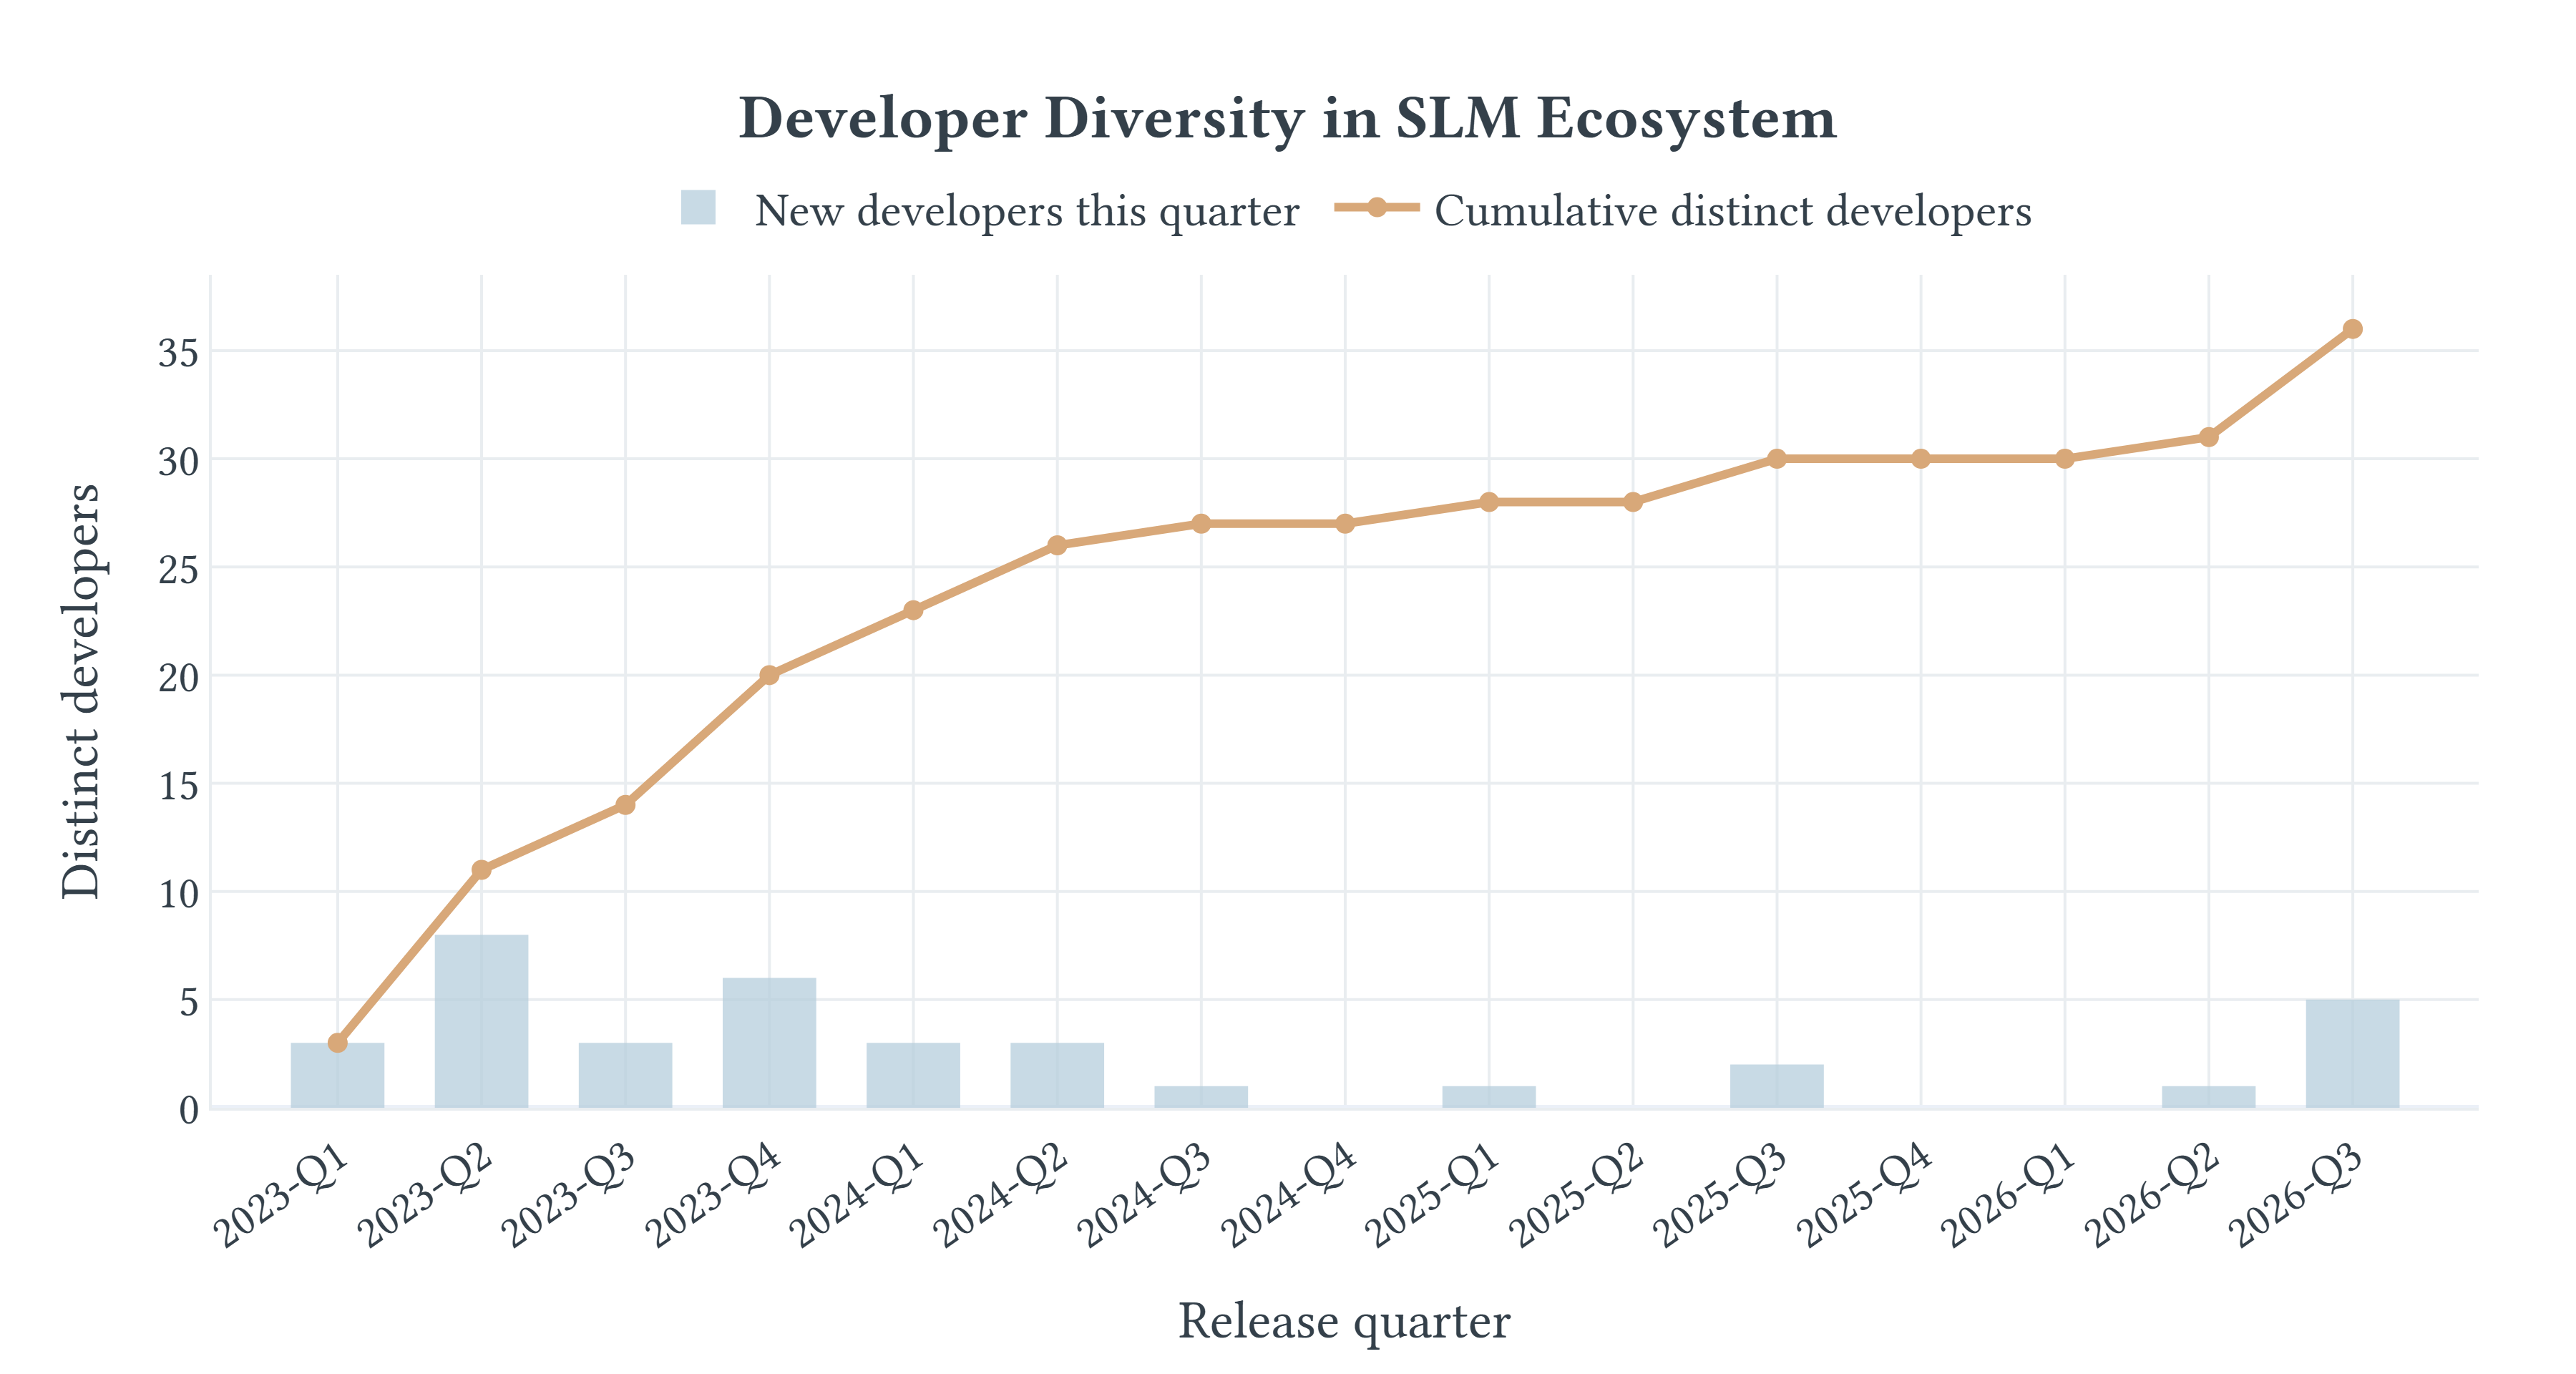
\includegraphics[width=\linewidth]{paper_slm_developer_diversity_timeline.png}
  \caption{Cumulative distinct developers releasing documented SLM variants (line) and new developers per quarter (bars).}
  \Description{Combination chart with bars showing the number of new developers releasing their first documented small language model in each quarter, overlaid with a line showing the cumulative count of distinct developers.}
  \label{fig:developer_diversity}
\end{figure}

\begin{figure}[ht]
  \centering
  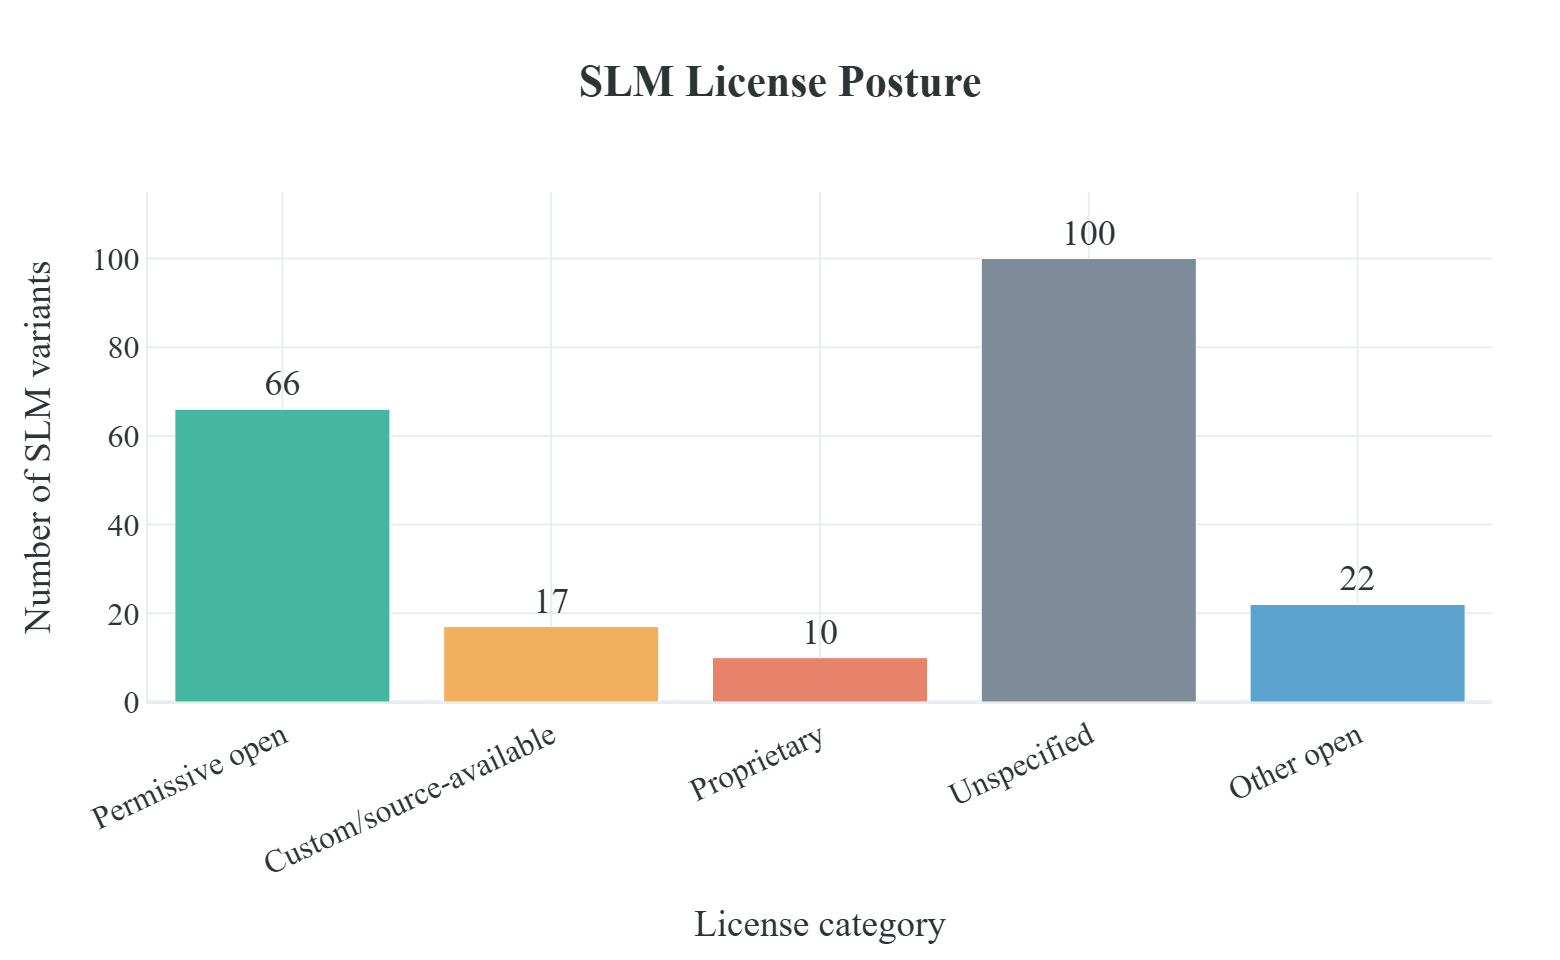
\includegraphics[width=0.78\linewidth]{paper_slm_license_posture.png}
  \caption{License posture of documented SLM variants. Permissive open licenses (Apache-2.0, MIT) account for the plurality; ``unspecified'' entries are typically research checkpoints without an attached license file.}
  \Description{Bar chart of documented small language model variants by license category. Permissive open licenses, chiefly Apache 2.0 and MIT, form the plurality, followed by custom vendor licenses and unspecified research checkpoints.}
  \label{fig:license_posture}
\end{figure}

\subsection{Representative Family Reference}
\label{subsec:ecosystem_families}
Table~\ref{tab:ecosystem_families} lists the representative families tracked in the inventory, with their developers, size ranges, access, and the role each plays in the landscape.

\begin{table}[ht]
\centering
\caption{Representative model families tracked in the inventory.}
\label{tab:ecosystem_families}
\footnotesize\adjustbox{max width=\linewidth}{%
\begin{tabular}{lllll}
\toprule
\textbf{Family} & \textbf{Developer} & \textbf{Representative Versions} & \textbf{Access} & \textbf{Typical Role} \\
\midrule
Qwen2.5 / Qwen3 & Alibaba & 0.5B--14B dense, MoE variants & Open weights & Strong multilingual, math, and code performance \\
Phi-3 / Phi-4 & Microsoft & 3.8B mini variants, 14B reasoning & Open weights & Data-curated reasoning-focused SLMs \\
Gemma 2 / 3 / 3n & Google DeepMind & 1B--12B dense, mobile-first multimodal variants & Open weights & Distilled compact models \\
Llama 3.2 / 4 & Meta & 1B--3B edge models, larger MoE frontier models & Open weights & Broad deployment ecosystem from edge to server \\
SmolLM2 / SmolLM3 & Hugging Face & 135M--3B & Open weights & Lightweight, fully open research and edge baselines \\
DeepSeek distills & DeepSeek & 1.5B--14B distilled reasoning models & Open weights & Reasoning transfer into self-hosted sizes \\
Granite 3 / 4 & IBM & 2--8B dense; 4.0 hybrid Mamba-2/MoE (350M--32B, 1--9B active) & Open weights & Enterprise-friendly, tool-use and RAG focus \\
Falcon-H1 & TII & 0.5--34B parallel attention/Mamba-2 hybrid & Open weights & Long-context edge-to-server \\
LFM2 / LFM2.5 & Liquid AI & 230M--8.3B hybrid conv/attention, incl.\ 8B-A1B MoE & Open weights & CPU-oriented on-device models \\
MiniCPM & OpenBMB & Compact multimodal variants & Open weights & Edge multimodal use cases \\
Ling / Nemotron 3.5 / Laguna & inclusionAI / NVIDIA / Poolside & Small-active MoE, 3--13B active & Open weights & SLM-like per-token cost at LLM-like residency \\
Frontier API families & OpenAI / Anthropic / Google / xAI / others & API frontier models (see released inventory) & API only & High-end proprietary baselines and teacher models \\
\bottomrule
\end{tabular}%
}
\end{table}

\subsection{Classification Conventions}
\label{subsec:ecosystem_classification}
The inventory applies conditions C1 and C2 of Section~\ref{subsubsec:intro_def_operative} from the parameter counts each record carries:
\begin{itemize}
    \item A record enters the inventory when its \emph{active} parameter count is at or below roughly 20B (C1); dense models, for which active equals total, therefore enter at or below 20B total. C2 (total at or below 20B) then separates \glspl{slm} from small-active-parameter \glspl{moe}; both are listed, and only the former carry the paper's storage, resident-memory, and on-device claims.
    \item Where a source states no active-parameter count for a model it describes as a mixture of experts, the record is marked undisclosed rather than having active set equal to total. Nested legacy records are read from their active field.
    \item Per-layer-embedding ``effective'' sizes (Gemma~3n, Gemma~4 E2B/E4B) are not sparse activation; C1 is evaluated on the total and the effective size is kept as a note.
    \item M1 is satisfied when a developer source states size and architecture; the source check of \suppsec~\ref{subsec:source_verification} records which source that is. Records of undisclosed size, whatever their marketing, are kept in the comparison part of the file as \texttt{undisclosed}.
    \item Encoder-decoder models, derivative fine-tunes without a technical report, and API aliases are excluded by named editorial decision and kept under \texttt{models.excluded} with their reason.
\end{itemize}
The count history from 126 to the present 209 is given in \suppsec~\ref{subsec:count_history}, and the released changelog names every record added, moved, or removed at each step.

\subsection{Generated Variant Inventory}
\label{subsec:ecosystem_generated_inventory}
The following inventory is generated directly from \file{merged\_llm\_database.json} using \file{scripts/generate\_model\_tables.py}. Version~3.6 of the database covers 209 inventory records (179 \glspl{slm} and 30 small-active-parameter \glspl{moe}), 223 comparison records (104 of disclosed size that fail C1 and 119 of undisclosed size), and 7 excluded candidates, 439 records in total, for releases through 4~September 2026. Only the inventory is reproduced here (Table~\ref{tab:model_inventory_slm_by_year}), organized by release year and family, with total and, where different, active parameters given in the size column; the comparison records are in the released file.

Each record carries the fields \texttt{meets\_c1\_active\_le\_20b}, \texttt{meets\_c2\_total\_le\_20b}, \texttt{slm\_class}, \texttt{inclusion\_decision}, \texttt{developer\_source\_found}, and \texttt{source\_check}, so that a reader can recompute the inventory under a different threshold, restrict it to models satisfying both conditions, or audit each record's source.

{\footnotesize\noindent\textbf{Chronology.} \hyperref[tab:model_inventory_slm_by_year]{Inventory}: \hyperlink{model-year-slm-2026}{2026}, \hyperlink{model-year-slm-2025}{2025}, \hyperlink{model-year-slm-2024}{2024}, \hyperlink{model-year-slm-2023-and-earlier}{2023 and earlier}.\par}
% Auto-generated by scripts/generate_model_tables.py. Do not edit manually.
\begin{landscape}
{\scriptsize
\setlength{\tabcolsep}{4pt}
\renewcommand{\arraystretch}{1.15}
\begin{longtable}{@{}L{3.3cm}C{1.05cm}L{1.75cm}C{1.15cm}L{2.25cm}L{2.4cm}C{1.6cm}L{3.9cm}@{}}
\caption{Generated chronological small language model inventory from \texttt{merged\_llm\_database.json}, grouped by release year and family. Entries whose parameter column reads ``$N$B ($M$B act.)'' with $N > 20$ are small-active-parameter MoEs (C1 only), not SLMs, and are excluded from every storage and on-device claim.}\label{tab:model_inventory_slm_by_year}\\
\toprule
\textbf{Model} & \textbf{Access} & \textbf{Params} & \textbf{Context} & \textbf{Modalities} & \textbf{License} & \textbf{Release} & \textbf{Notes} \\ \midrule
\endfirsthead
\caption[]{Generated chronological small language model inventory continued.}\\
\toprule
\textbf{Model} & \textbf{Access} & \textbf{Params} & \textbf{Context} & \textbf{Modalities} & \textbf{License} & \textbf{Release} & \textbf{Notes} \\ \midrule
\endhead
\midrule \multicolumn{8}{r@{}}{\footnotesize\itshape continued on next page} \\
\endfoot
\bottomrule
\endlastfoot
\multicolumn{8}{@{}l}{\hypertarget{model-year-slm-2026}{\textbf{2026}}} \\ \midrule
\multicolumn{8}{@{}l}{\textit{Qwen3.5} --- Alibaba (Qwen3.5 (Mar 2026)) \href{https://qwen.ai/blog?id=qwen3.5}{[family page]}} \\*
\href{https://huggingface.co/Qwen/Qwen3.5-0.8B}{Qwen3.5-0.8B} & OW & 0.8B & 256K & Text+Vision+Video & Apache 2.0 & 2026-03-02 & ultra-lightweight multimodal; on-device \\
\href{https://huggingface.co/Qwen/Qwen3.5-2B}{Qwen3.5-2B} & OW & 2B & 256K & Text+Vision+Video & Apache 2.0 & 2026-03-02 & on-device multimodal chat; edge AI \\
\href{https://huggingface.co/Qwen/Qwen3.5-4B}{Qwen3.5-4B} & OW & 4B & 256K & Text+Vision+Video & Apache 2.0 & 2026-03-02 & mobile multimodal assistant; agentic coding \\
\href{https://huggingface.co/Qwen/Qwen3.5-9B}{Qwen3.5-9B} & OW & 9B & 256K & Text+Vision+Video & Apache 2.0 & 2026-03-02 & strong multimodal SLM; coding \\
\href{https://huggingface.co/Qwen/Qwen3.5-35B-A3B}{Qwen3.5-35B-A3B} & OW & 35B (3B act.) & 256K & Text+Vision & Apache 2.0 & 2026-02-16 & efficient MoE for edge/server; multimodal reasoning \\
\href{https://huggingface.co/Qwen/Qwen3.5-122B-A10B}{Qwen3.5-122B-A10B} & OW & 122B (10B act.) & 256K & Text+Vision & Apache 2.0 & 2026-02-16 & strong MoE reasoning; locally runnable flagship \\
\href{https://huggingface.co/Qwen/Qwen3.5-397B-A17B}{Qwen3.5-397B-A17B} & Both & 397B (17B act.) & 256K & Text+Vision & Apache 2.0 & 2026-02-16 & flagship open-weight multimodal; 201 languages \\
\multicolumn{8}{@{}l}{\textit{AFM} --- Apple (AFM) \href{https://machinelearning.apple.com/research/introducing-apple-foundation-models}{[family page]}} \\*
\href{https://machinelearning.apple.com/research/introducing-third-generation-of-apple-foundation-models}{Apple AFM 3 Core Advanced} & API & 20B (1-4B act.) & 64K & Text+Vision & Proprietary & 2026-06-08 & on-device assistant; multimodal understanding \\
\multicolumn{8}{@{}l}{\textit{Command} --- Cohere (Command) \href{https://cohere.com/blog/command-r7b}{[family page]}} \\*
\href{https://huggingface.co/CohereLabs/North-Mini-Code-1.0}{North Mini Code 1.0} & OW & 30B (3B act.) & 250K & Text & CC-BY-NC (Cohere Labs) & 2026-06-17 & coding; agentic coding \\
\multicolumn{8}{@{}l}{\textit{DeepSeek} --- DeepSeek (DeepSeek) \href{https://huggingface.co/deepseek-ai}{[family page]}} \\*
\href{https://huggingface.co/deepseek-ai/DeepSeek-V4-Flash-Vision-Exp}{DeepSeek V4 Flash Vision Exp} & OW & 284B (13B act.) & 1M & Text+Vision & See source & 2026-08-21 & vision; long context \\
\href{https://huggingface.co/deepseek-ai/DeepSeek-V4-Flash-0731}{DeepSeek V4 Flash 0731} & OW & 284B (13B act.) & 1280K & Text & See source & 2026-07-31 & general; long context \\
\multicolumn{8}{@{}l}{\textit{Dots} --- Dots Studio (Dots3-Note Preview (Aug 2026)) \href{https://openrouter.ai/dots-studio/dots-3-note-preview}{[family page]}} \\*
\href{https://huggingface.co/dots-studio/dots3-note-prev}{Dots3-Note Preview} & OW & 280B (16B act.) & 500K & Text & Apache 2.0 & 2026-08-14 & note taking; general \\
\multicolumn{8}{@{}l}{\textit{Gemma 4} --- Google DeepMind} \\*
\href{https://huggingface.co/google/gemma-4-26B}{Gemma 4 26B (MoE)} & OW & 26B (3.8B act.) & 128K & Text+Vision & Apache 2.0 & 2026-04-02 & reasoning; multimodal \\
\href{https://huggingface.co/google/gemma-4-E2B}{Gemma 4 E2B} & OW & \textasciitilde{}5B & 128K & Text+Vision+Audio & Apache 2.0 & 2026-04-02 & on-device; multimodal \\
\href{https://huggingface.co/google/gemma-4-E4B}{Gemma 4 E4B} & OW & \textasciitilde{}8B & 128K & Text+Vision+Audio & Apache 2.0 & 2026-04-02 & multimodal; reasoning \\
\href{https://huggingface.co/google/gemma-4-12b}{Gemma 4 12B} & OW & 12B & 256K & Text+Vision+Audio & Apache 2.0 & 2026-04-02 & multimodal; reasoning \\
\multicolumn{8}{@{}l}{\textit{Granite 4} --- IBM} \\*
\href{https://huggingface.co/ibm-granite/granite-4.2-3b}{Granite 4.2 3B} & OW & 3B & 128K & Text & Apache 2.0 & 2026-08-25 & reasoning; on-device \\
\href{https://huggingface.co/ibm-granite/granite-4.2-8b}{Granite 4.2 8B} & OW & 8B & 128K & Text & Apache 2.0 & 2026-08-25 & reasoning; agentic \\
\href{https://huggingface.co/ibm-granite/granite-4.1-3b}{Granite 4.1 3B} & OW & 3B & 128K & Text & Apache 2.0 & 2026-04-29 & enterprise; on-device \\
\href{https://huggingface.co/ibm-granite/granite-4.1-8b}{Granite 4.1 8B} & OW & 8B & 128K & Text & Apache 2.0 & 2026-04-29 & enterprise; agentic \\
\multicolumn{8}{@{}l}{\textit{LFM2} --- Liquid AI} \\*
\href{https://huggingface.co/LiquidAI/LFM2.5-2.6B}{LFM2.5-2.6B} & Both & 2.69B & 128K & Text & LFM1.0 & 2026-08-04 & agentic workflows; data extraction \\
\href{https://www.liquid.ai/blog/lfm2-5-8b-a1b}{LFM2.5-8B-A1B} & OW & 8.3B (1.5B act.) & 128K & Text & LFM1.0 & 2026-05-28 & on-device; tool calling \\
\href{https://www.liquid.ai/blog/lfm2-5-350m-no-size-left-behind}{LFM2.5-350M} & OW & 350M & 128K & Text & LFM1.0 & 2026 & on-device; edge \\
\href{https://www.liquid.ai/models}{LFM2.5-1.2B} & OW & 1.2B & 128K & Text & LFM1.0 & 2026 & on-device; edge \\
\href{https://www.liquid.ai/models}{LFM2.5-Audio-1.5B} & OW & 1.5B & -- & Text+Audio & LFM1.0 & 2026 & on-device speech; transcription \\
\href{https://www.liquid.ai/models}{LFM2.5-VL-3B} & OW & 3B & -- & Text+Vision & LFM1.0 & 2026 & on-device VLM; document extraction \\
\multicolumn{8}{@{}l}{\textit{Mistral Small} --- Mistral AI (Mistral Small 4 (Mar 2026)) \href{https://mistral.ai/news/mistral-small-4}{[family page]}} \\*
\href{https://huggingface.co/mistralai/Mistral-Small-4-119B-2603}{Mistral Small 4 (119B)} & Both & 119B (6.5B act.) & 256K & Text+Vision & Apache 2.0 & 2026-03-16 & hybrid reasoning; coding \\
\multicolumn{8}{@{}l}{\textit{NVIDIA Nemotron} --- NVIDIA (Nemotron 3 Super (Mar 2026)) \href{https://developer.nvidia.com/blog/introducing-nemotron-3-super-an-open-hybrid-mamba-transformer-moe-for-agentic-reasoning/}{[family page]}} \\*
\href{https://huggingface.co/nvidia/NVIDIA-NemotronLabs-VoiceChat-11B}{NemotronLabs VoiceChat 11B} & OW & 11B & 128K & Text+Audio & NVIDIA Custom & 2026-08-03 & voice interaction; on-device speech \\
\href{https://huggingface.co/nvidia/NVIDIA-Nemotron-3-Super-120B-A12B-BF16}{Nemotron 3 Super} & OW & 120B (12B act.) & 1M & Text & NVIDIA Open Model License & 2026-03 & open hybrid Mamba-Transformer MoE; agentic reasoning \\
\multicolumn{8}{@{}l}{\textit{Nemotron} --- NVIDIA (Nemotron) \href{https://arxiv.org/abs/2402.16819}{[family page]}} \\*
\href{https://huggingface.co/nvidia/NVIDIA-Nemotron-3.5-Lightning-30B-A3B-BF16}{Nemotron 3.5 Lightning 30B-A3B} & OW & 30B (3B act.) & 256K & Text & NVIDIA Open Model License & 2026-08-11 & agentic execution layer; high-volume tool calling \\
\href{https://huggingface.co/nvidia/Nemotron-3.5-Content-Safety}{Nemotron 3.5 Content Safety} & OW & 4B & 128K & Text+Vision & NVIDIA Open Model License & 2026-06-04 & guardrails; content moderation \\
\multicolumn{8}{@{}l}{\textit{Nex-N2} --- Nex AGI (Nex-N2-Mini (Jun 2026)) \href{https://huggingface.co/nex-agi/Nex-N2-Pro}{[family page]}} \\*
\href{https://huggingface.co/nex-agi/Nex-N2-Pro}{Nex-N2-Pro} & OW & 397B (17B act.) & 256K & Text+Vision & See source & 2026-06-08 & agentic; coding \\
\multicolumn{8}{@{}l}{\textit{Laguna} --- Poolside (Laguna S 2.1 (Jul 2026)) \href{https://poolside.ai/}{[family page]}} \\*
\href{https://huggingface.co/poolside/Laguna-S-2.1}{Laguna S 2.1} & OW & 118B (8B act.) & 1M & Text & See source & 2026-07-21 & coding agent \\
\href{https://huggingface.co/poolside/Laguna-XS-2.1}{Laguna XS 2.1} & OW & 33B (3B act.) & 256K & Text & See source & 2026-07-02 & coding agent \\
\multicolumn{8}{@{}l}{\textit{Hunyuan} --- Tencent (Hunyuan) \href{https://huggingface.co/tencent/Tencent-Hunyuan-Large}{[family page]}} \\*
\href{https://huggingface.co/tencent/Hy-MT2-1.8B}{Hy-MT2-1.8B} & OW & 1.8B & 8K & Text & Tencent Hunyuan License & 2026-08-20 & translation; on-device \\
\href{https://huggingface.co/tencent/Hy-MT2-30B-A3B}{Hy-MT2-30B-A3B} & OW & 30B (3B act.) & 8K & Text & Tencent Hunyuan License & 2026-08-20 & translation \\
\href{https://huggingface.co/tencent/Hy-MT2-7B}{Hy-MT2-7B} & OW & 7B & 8K & Text & Tencent Hunyuan License & 2026-08-19 & translation; Lang: 33 language pairs + 5 dialect/minority pairs \\
\multicolumn{8}{@{}l}{\textit{Inkling} --- Thinking Machines Lab (Inkling Small (Jul 2026)) \href{https://huggingface.co/thinkingmachines/Inkling}{[family page]}} \\*
\href{https://huggingface.co/thinkingmachines/Inkling-Small}{Inkling Small} & OW & 276B (12B act.) & 1M & Text+Vision & See source & 2026-07-30 & general; multimodal \\
\multicolumn{8}{@{}l}{\textit{MiMo} --- Xiaomi (MiMo-V2-Pro (Mar 2026)) \href{https://mimo.xiaomi.com/mimo-v2-pro}{[family page]}} \\*
\href{https://huggingface.co/XiaomiMiMo/MiMo-V2-Flash}{MiMo-V2-Flash} & OW & 309B (15B act.) & 256K & Text & Undisclosed & 2026 & high-throughput coding agents; production serving \\
\multicolumn{8}{@{}l}{\textit{Ling} --- inclusionAI (Ling-1T (2026)) \href{https://huggingface.co/01ai/Ling-1T}{[family page]}} \\*
\href{https://huggingface.co/inclusionAI/Ling-3.0-flash-Fin}{Ling 3.0 Flash Fin} & OW & 124B (5.1B act.) & 256K & Text & MIT & 2026-08-27 & finance \\
\href{https://huggingface.co/inclusionAI/Ling-3.0-flash}{Ling 3.0 Flash} & OW & 124B (5.1B act.) & 256K & Text & See source & 2026-07-23 & general; agentic \\
\addlinespace[3pt]
\multicolumn{8}{@{}l}{\hypertarget{model-year-slm-2025}{\textbf{2025}}} \\ \midrule
\multicolumn{8}{@{}l}{\textit{Qwen} --- Alibaba (Qwen) \href{https://github.com/QwenLM/Qwen}{[family page]}} \\*
\href{https://huggingface.co/Qwen/Qwen2.5-Omni-7B}{Qwen2.5-Omni-7B} & OW & 7B & -- & Text+Audio+Video+Image & See source & 2025-03-26 & omni-modal; text and audio output \\
\href{https://huggingface.co/Qwen/Qwen2.5-VL-7B-Instruct}{Qwen2.5-VL-7B} & OW & 7B & -- & Text+Video+Image & See source & 2025-01-22 & active \\
\multicolumn{8}{@{}l}{\textit{Qwen3} --- Alibaba (Qwen3 (Apr 2025)) \href{https://github.com/QwenLM/Qwen3}{[family page]}} \\*
\href{https://huggingface.co/Qwen/Qwen3-4B-Instruct-2507}{Qwen3-4B-Instruct-2507} & OW & 4B & 128K & Text & Apache 2.0 & 2025-07 & improved instruction following; non-thinking mode optimised \\
\href{https://huggingface.co/Qwen/Qwen3-0.6B}{Qwen3-0.6B} & OW & 0.6B & 32K & Text & Apache 2.0 & 2025-04-29 & edge inference; IoT \\
\href{https://huggingface.co/Qwen/Qwen3-1.7B}{Qwen3-1.7B} & OW & 1.7B & 32K & Text & Apache 2.0 & 2025-04-29 & mobile inference; Q\&A \\
\href{https://huggingface.co/Qwen/Qwen3-30B-A3B}{Qwen3-30B-A3B} & OW & 30B (3B act.) & 128K & Text & Apache 2.0 & 2025-04-29 & MoE efficiency; broad capability in tiny footprint \\
\href{https://huggingface.co/Qwen/Qwen3-4B-Instruct}{Qwen3-4B-Instruct} & OW & 4B & 128K & Text & Apache 2.0 & 2025-04-29 & on-device chat; coding \\
\href{https://huggingface.co/Qwen/Qwen3-8B-Instruct}{Qwen3-8B-Instruct} & OW & 8B & 128K & Text & Apache 2.0 & 2025-04-29 & single-GPU inference; reasoning \\
\href{https://huggingface.co/Qwen/Qwen3-14B-Instruct}{Qwen3-14B-Instruct} & OW & 14B & 128K & Text & Apache 2.0 & 2025-04-29 & high-quality on-premise chat; coding \\
\multicolumn{8}{@{}l}{\textit{AFM} --- Apple (AFM) \href{https://machinelearning.apple.com/research/introducing-apple-foundation-models}{[family page]}} \\*
\href{https://arxiv.org/abs/2507.13575}{Apple Foundation Model (On-Device, 2nd gen)} & API & \textasciitilde{}3B & 64K & Text+Vision & Proprietary & 2025-06-09 & on-device assistant; writing tools \\
\multicolumn{8}{@{}l}{\textit{DeepSeek R1-Distill} --- DeepSeek (R1-Distill (Jan 2025)) \href{https://huggingface.co/deepseek-ai}{[family page]}} \\*
\href{https://huggingface.co/deepseek-ai/DeepSeek-R1-Distill-Qwen-1.5B}{DeepSeek-R1-Distill-Qwen-1.5B} & OW & 1.5B & 128K & Text & MIT & 2025-01-20 & reasoning at ultra-small scale; math \\
\href{https://huggingface.co/deepseek-ai/DeepSeek-R1-Distill-Qwen-7B}{DeepSeek-R1-Distill-Qwen-7B} & OW & 7B & 128K & Text & MIT & 2025-01-20 & chain-of-thought reasoning; coding \\
\href{https://huggingface.co/deepseek-ai/DeepSeek-R1-Distill-Llama-8B}{DeepSeek-R1-Distill-Llama-8B} & OW & 8B & 128K & Text & MIT & 2025-01-20 & reasoning on Llama 3 base; on-premise \\
\href{https://huggingface.co/deepseek-ai/DeepSeek-R1-Distill-Qwen-14B}{DeepSeek-R1-Distill-Qwen-14B} & OW & 14B & 128K & Text & MIT & 2025-01-20 & strong reasoning 14B; top distill for coding \\
\multicolumn{8}{@{}l}{\textit{Gemma 3} --- Google DeepMind (Gemma 3 (Mar 2025)) \href{https://huggingface.co/blog/gemma3}{[family page]}} \\*
\href{https://huggingface.co/google/gemma-3-270m-it}{Gemma 3 270M-IT} & OW & 270M & 32K & Text & Google Gemma License & 2025-03 & ultra-lightweight prototyping; experiments \\
\href{https://huggingface.co/google/gemma-3-1b-it}{Gemma 3 1B-IT} & OW & 1B & 32K & Text & Google Gemma License & 2025-03 & on-device mobile inference; lightweight Q\&A \\
\href{https://huggingface.co/google/gemma-3-4b-it}{Gemma 3 4B-IT} & OW & 4B & 128K & Text+Vision & Google Gemma License & 2025-03 & multimodal on-device; image understanding \\
\href{https://huggingface.co/google/gemma-3-12b-it}{Gemma 3 12B-IT} & OW & 12B & 128K & Text+Vision & Google Gemma License & 2025-03 & high-quality assistant; 140+ languages \\
\multicolumn{8}{@{}l}{\textit{Gemma 3n} --- Google DeepMind (Gemma-3n (2025)) \href{https://ai.google.dev/gemma/docs/gemma-3n}{[family page]}} \\*
\href{https://huggingface.co/google/gemma-3n-E2B-it}{Gemma-3n-E2B-IT} & OW & \textasciitilde{}5B & 32K & Text+Vision+Audio+Video & Google Gemma License & 2025 & mobile-first multimodal; on-device speech/vision/text \\
\href{https://huggingface.co/google/gemma-3n-E4B-it}{Gemma-3n-E4B-IT} & OW & \textasciitilde{}8B & 32K & Text+Vision+Audio+Video & Google Gemma License & 2025 & higher-accuracy mobile multimodal; edge devices \\
\multicolumn{8}{@{}l}{\textit{SmolLM} --- Hugging Face (SmolLM3-3B (2025)) \href{https://huggingface.co/HuggingFaceTB/SmolLM3-3B}{[family page]}} \\*
\href{https://huggingface.co/HuggingFaceTB/SmolLM3-3B}{SmolLM3-3B} & OW & 3B & 64K & Text & Apache 2.0 & 2025 & dual-mode reasoning; tool calling \\
\multicolumn{8}{@{}l}{\textit{Granite} --- IBM (Granite) \href{https://huggingface.co/ibm-granite}{[family page]}} \\*
\href{https://huggingface.co/ibm-granite/granite-3.2-2b-instruct}{Granite 3.2-2B} & OW & 2B & 125K & Text & See source & 2025-02-26 & Thinking mode; 128K context \\
\href{https://huggingface.co/ibm-granite/granite-3.2-8b-instruct}{Granite 3.2-8B} & OW & 8B & 125K & Text & See source & 2025-02-26 & Thinking mode (chain-of-thought); 128K context \\
\multicolumn{8}{@{}l}{\textit{IBM Granite} --- IBM (Granite 3.3 (Apr 2025)) \href{https://huggingface.co/ibm-granite}{[family page]}} \\*
\href{https://huggingface.co/ibm-granite/granite-4.0-nano-350m}{Granite 4.0 Nano 350M} & OW & 350M & 128K & Text & Apache 2.0 & 2025-10-28 & on-device; browser \\
\href{https://huggingface.co/ibm-granite/granite-4.0-nano-1b}{Granite 4.0 Nano 1B} & OW & 1B & 128K & Text & Apache 2.0 & 2025-10-28 & on-device; browser \\
\href{https://huggingface.co/ibm-granite/granite-4.0-h-tiny}{Granite 4.0 H-Tiny} & OW & 7B (1B act.) & 128K & Text & Apache 2.0 & 2025-10-02 & low-latency; agentic \\
\href{https://huggingface.co/ibm-granite/granite-4.0-h-micro}{Granite 4.0 H-Micro} & OW & 3B & 128K & Text & Apache 2.0 & 2025-10-02 & edge; tool use \\
\href{https://huggingface.co/ibm-granite/granite-4.0-micro}{Granite 4.0 Micro} & OW & 3B & 128K & Text & Apache 2.0 & 2025-10-02 & edge; RAG \\
\href{https://huggingface.co/ibm-granite/granite-4.0-h-small}{Granite 4.0 H-Small} & OW & 32B (9B act.) & 128K & Text & Apache 2.0 & 2025-10-02 & enterprise; agentic \\
\href{https://huggingface.co/ibm-granite/granite-3.3-2b-instruct}{Granite 3.3-2B-Instruct} & OW & 2B & 128K & Text & Apache 2.0 & 2025-04 & enterprise NLP; governed AI \\
\href{https://huggingface.co/ibm-granite/granite-3.3-8b-instruct}{Granite 3.3-8B-Instruct} & OW & 8B & 128K & Text & Apache 2.0 & 2025-04 & enterprise reasoning; Fill-in-Middle code \\
\multicolumn{8}{@{}l}{\textit{LFM2} --- Liquid AI} \\*
\href{https://huggingface.co/LiquidAI/LFM2-8B-A1.5B}{LFM2-8B-A1.5B (MoE)} & OW & 8.3B (1.5B act.) & 32K & Text & LFM Open License v1.0 & 2025-08 & on-device; agentic \\
\href{https://huggingface.co/LiquidAI/LFM2-2.6B}{LFM2-2.6B} & OW & 2.6B & 32K & Text & LFM Open License v1.0 & 2025-08 & on-device \\
\href{https://huggingface.co/LiquidAI/LFM2-350M}{LFM2-350M} & OW & 350M & 32K & Text & LFM Open License v1.0 & 2025-07-10 & on-device; low latency \\
\href{https://huggingface.co/LiquidAI/LFM2-700M}{LFM2-700M} & OW & 700M & 32K & Text & LFM Open License v1.0 & 2025-07-10 & on-device \\
\href{https://huggingface.co/LiquidAI/LFM2-1.2B}{LFM2-1.2B} & OW & 1.2B & 32K & Text & LFM Open License v1.0 & 2025-07-10 & on-device; agentic \\
\multicolumn{8}{@{}l}{\textit{Llama 4} --- Meta AI (Llama 4 Maverick (Apr 2025)) \href{https://ai.meta.com/blog/llama-4-multimodal-intelligence/}{[family page]}} \\*
\href{https://huggingface.co/meta-llama/Llama-4-Maverick-17B-128E-Instruct}{Llama 4 Maverick} & Both & 400B (17B act.) & 10M & Text+Vision & Llama 4 Community License & 2025-04-05 & image understanding; coding \\
\href{https://huggingface.co/meta-llama/Llama-4-Scout-17B-16E-Instruct}{Llama 4 Scout} & Both & 109B (17B act.) & 10M & Text+Vision & Llama 4 Community License & 2025-04-05 & extreme long-context; single H100 runnable \\
\multicolumn{8}{@{}l}{\textit{BitNet} --- Microsoft (BitNet) \href{https://arxiv.org/abs/2402.17764}{[family page]}} \\*
\href{https://huggingface.co/microsoft/bitnet-b1.58-2B-4T}{BitNet b1.58 2B4T} & OW & 2B & -- & Text & MIT & 2025-04-16 & 1-bit LLM (ternary weights: -1, 0, 1); Extreme efficiency \\
\multicolumn{8}{@{}l}{\textit{Phi-4} --- Microsoft (Phi-4-reasoning-plus (Apr 2025)) \href{https://huggingface.co/microsoft/phi-4}{[family page]}} \\*
\href{https://huggingface.co/microsoft/Phi-4-mini-flash-reasoning}{Phi-4-mini-flash-reasoning} & OW & 3.8B & 128K & Text & MIT & 2025-04 & fast reasoning; edge agents \\
\href{https://huggingface.co/microsoft/Phi-4-mini-reasoning}{Phi-4-mini-reasoning} & OW & 3.8B & 128K & Text & MIT & 2025-04 & chain-of-thought reasoning; math \\
\href{https://huggingface.co/microsoft/Phi-4-reasoning}{Phi-4-reasoning} & OW & 14B & 128K & Text & MIT & 2025-04 & complex reasoning; STEM \\
\href{https://huggingface.co/microsoft/Phi-4-reasoning-plus}{Phi-4-reasoning-plus} & OW & 14B & 128K & Text & MIT & 2025-04 & RL-trained reasoning; math olympiad-level \\
\href{https://huggingface.co/microsoft/Phi-4-mini-instruct}{Phi-4-mini-instruct} & OW & 3.8B & 128K & Text & MIT & 2025-02 & on-device chat; function calling \\
\multicolumn{8}{@{}l}{\textit{Ministral} --- Mistral AI (Ministral-3B (Dec 2025)) \href{https://docs.mistral.ai/getting-started/models}{[family page]}} \\*
\href{https://huggingface.co/mistralai/Ministral-3-14B-Instruct-2512}{Ministral 3 (14B)} & OW & 14B & -- & Text+Vision & See source & 2025-12-02 & edge deployment; multimodal \\
\href{https://huggingface.co/mistralai/Ministral-3B-instruct-2512}{Ministral-3B-Instruct-2512} & OW & 3.8B & 256K & Text+Vision & Apache 2.0 & 2025-12 & tiny multimodal; function calling \\
\multicolumn{8}{@{}l}{\textit{Voxtral} --- Mistral AI (Voxtral) \href{https://mistral.ai/models}{[family page]}} \\*
\href{https://huggingface.co/mistralai/Voxtral-Mini-3B-2507}{Voxtral Mini 3B} & OW & 4.7B & -- & Text+Audio & Apache 2.0 & 2025-07-15 & speech understanding; transcription \\
\multicolumn{8}{@{}l}{\textit{Nemotron} --- NVIDIA (Nemotron) \href{https://arxiv.org/abs/2402.16819}{[family page]}} \\*
\href{https://huggingface.co/nvidia/Nemotron-3-Nano-30B}{Nemotron 3 Nano-30B} & OW & 30B & -- & Text & See source & 2025-12-15 & hybrid Mamba-Transformer MoE; 1M context \\
\href{https://huggingface.co/nvidia/NVIDIA-Nemotron-Nano-9B-v2}{NVIDIA Nemotron Nano 2} & OW & 9B & 128K & Text & See source & 2025-08-18 & on-device; efficient \\
\multicolumn{8}{@{}l}{\textit{GPT-OSS} --- OpenAI (gpt-oss-120b (2025)) \href{https://openai.com/index/introducing-gpt-oss/}{[family page]}} \\*
\href{https://huggingface.co/openai/gpt-oss-20b}{gpt-oss-20b} & OW & 21B (3.6B act.) & 128K & Text & Apache 2.0 & 2025 & edge reasoning; 16GB device inference \\
\href{https://huggingface.co/openai/gpt-oss-120b}{gpt-oss-120b} & OW & 117B (5.1B act.) & 128K & Text & Apache 2.0 & 2025 & open-weight reasoning; near o4-mini parity \\
\multicolumn{8}{@{}l}{\textit{MiniCPM} --- OpenBMB (MiniCPM-V 4.5 (2025)) \href{https://github.com/OpenBMB/MiniCPM-V}{[family page]}} \\*
\href{https://huggingface.co/openbmb/MiniCPM-V-4\_5}{MiniCPM-V 4.5} & OW & \textasciitilde{}8B & 32K & Text+Vision & Apache 2.0 & 2025 & mobile vision-language; on-device VQA \\
\href{https://github.com/OpenBMB/MiniCPM-o}{MiniCPM-o 3.0} & OW & \textasciitilde{}9B & 32K & Text+Vision+Audio & Apache 2.0 & 2025 & end-to-end multimodal on-device; live streaming \\
\multicolumn{8}{@{}l}{\textit{InternLM} --- Shanghai AI Laboratory (InternLM) \href{https://github.com/InternLM/InternLM}{[family page]}} \\*
\href{https://huggingface.co/internlm/internlm3-8b-instruct}{InternLM3-8B} & OW & 8B & 32K & Text & See source & 2025-01-09 & Reasoning via deep thinking; Knowledge-rich training pipeline \\
\multicolumn{8}{@{}l}{\textit{Falcon-H1} --- Technology Innovation Institute} \\*
\href{https://huggingface.co/tiiuae/Falcon-H1-0.5B-Instruct}{Falcon-H1-0.5B} & OW & 0.5B & 256K & Text & Falcon-LLM License 2.0 & 2025-07-31 & edge; long context \\
\href{https://huggingface.co/tiiuae/Falcon-H1-1.5B-Instruct}{Falcon-H1-1.5B} & OW & 1.5B & 256K & Text & Falcon-LLM License 2.0 & 2025-07-31 & edge; long context \\
\href{https://huggingface.co/tiiuae/Falcon-H1-3B-Instruct}{Falcon-H1-3B} & OW & 3B & 256K & Text & Falcon-LLM License 2.0 & 2025-07-31 & general; long context \\
\href{https://huggingface.co/tiiuae/Falcon-H1-7B-Instruct}{Falcon-H1-7B} & OW & 7B & 256K & Text & Falcon-LLM License 2.0 & 2025-07-31 & general; long context \\
\addlinespace[3pt]
\multicolumn{8}{@{}l}{\hypertarget{model-year-slm-2024}{\textbf{2024}}} \\ \midrule
\multicolumn{8}{@{}l}{\textit{Yi} --- 01.AI (Yi) \href{https://huggingface.co/01-ai/Yi-6B}{[family page]}} \\*
\href{https://huggingface.co/01-ai/Yi-1.5-6B}{Yi-1.5-6B} & OW & 6B & -- & Text & See source & 2024-05-13 & legacy \\
\href{https://huggingface.co/01-ai/Yi-1.5-9B}{Yi-1.5-9B} & OW & 9B & -- & Text & See source & 2024-05-13 & legacy \\
\multicolumn{8}{@{}l}{\textit{Qwen} --- Alibaba (Qwen) \href{https://github.com/QwenLM/Qwen}{[family page]}} \\*
\href{https://huggingface.co/Qwen/Qwen2.5-Coder-1.5B-Instruct}{Qwen2.5-Coder-1.5B} & OW & 1.5B & -- & Text & See source & 2024-11-12 & compact coding model \\
\href{https://huggingface.co/Qwen/Qwen2.5-14B}{Qwen2.5-14B} & OW & 14B & -- & Text & See source & 2024-09-19 & active \\
\href{https://huggingface.co/Qwen/Qwen2-VL-7B-Instruct}{Qwen2-VL-7B} & OW & 7B & -- & Text+Video+Image & See source & 2024-08-28 & vision-language; video understanding \\
\href{https://huggingface.co/Qwen/Qwen2-Audio-7B-Instruct}{Qwen2-Audio-7B} & OW & 7B & -- & Text+Audio & See source & 2024-08-09 & audio understanding; speech recognition \\
\href{https://huggingface.co/Qwen/Qwen2-0.5B}{Qwen2-0.5B} & OW & 0.5B & -- & Text & See source & 2024-06-07 & active \\
\href{https://huggingface.co/Qwen/Qwen2-1.5B}{Qwen2-1.5B} & OW & 1.5B & -- & Text & See source & 2024-06-07 & active \\
\href{https://huggingface.co/Qwen/Qwen2-7B}{Qwen2-7B} & OW & 7B & -- & Text & See source & 2024-06-07 & active \\
\href{https://huggingface.co/Qwen/Qwen2-57B-A14B}{Qwen2-57B-A14B} & OW & 57B & -- & Text & See source & 2024-06-07 & active \\
\href{https://huggingface.co/Qwen/Qwen1.5-MoE-A2.7B}{Qwen1.5-MoE-A2.7B} & OW & 14.3B & -- & Text & See source & 2024-03-28 & MoE architecture; efficient \\
\href{https://huggingface.co/Qwen/Qwen1.5-0.5B}{Qwen1.5-0.5B} & OW & 0.5B & -- & Text & See source & 2024-02-05 & legacy \\
\href{https://huggingface.co/Qwen/Qwen1.5-7B}{Qwen1.5-7B} & OW & 7B & -- & Text & See source & 2024-02-05 & legacy \\
\href{https://huggingface.co/Qwen/Qwen1.5-14B}{Qwen1.5-14B} & OW & 14B & -- & Text & See source & 2024-02-05 & legacy \\
\multicolumn{8}{@{}l}{\textit{Qwen2.5} --- Alibaba (Qwen2.5 (Sep 2024)) \href{https://huggingface.co/Qwen}{[family page]}} \\*
\href{https://huggingface.co/Qwen/Qwen2.5-0.5B-Instruct}{Qwen2.5-0.5B-Instruct} & OW & 0.5B & 32K & Text & Apache 2.0 & 2024-09-19 & extreme edge/IoT; classification \\
\href{https://huggingface.co/Qwen/Qwen2.5-1.5B-Instruct}{Qwen2.5-1.5B-Instruct} & OW & 1.5B & 32K & Text & Apache 2.0 & 2024-09-19 & edge NLP; lightweight assistants \\
\href{https://huggingface.co/Qwen/Qwen2.5-3B-Instruct}{Qwen2.5-3B-Instruct} & OW & 3B & 32K & Text & Apache 2.0 & 2024-09-19 & mobile chat; summarization \\
\href{https://huggingface.co/Qwen/Qwen2.5-7B-Instruct}{Qwen2.5-7B-Instruct} & OW & 7B & 128K & Text & Apache 2.0 & 2024-09-19 & general assistant; coding \\
\multicolumn{8}{@{}l}{\textit{Qwen2.5-Coder} --- Alibaba (Qwen2.5-Coder (Nov 2024)) \href{https://huggingface.co/Qwen/Qwen2.5-Coder-7B-Instruct}{[family page]}} \\*
\href{https://huggingface.co/Qwen/Qwen2.5-Coder-7B-Instruct}{Qwen2.5-Coder-7B-Instruct} & OW & 7B & 128K & Text+Code & Apache 2.0 & 2024-11 & code generation; debugging \\
\href{https://huggingface.co/Qwen/Qwen2.5-Coder-14B-Instruct}{Qwen2.5-Coder-14B-Instruct} & OW & 14B & 128K & Text+Code & Apache 2.0 & 2024-11 & advanced code assistant; agentic code tasks \\
\multicolumn{8}{@{}l}{\textit{OLMo} --- Allen Institute for AI (Ai2) (OLMo) \href{https://allenai.org/olmo}{[family page]}} \\*
\href{https://huggingface.co/allenai/OLMo-2-1124-7B}{OLMo 2-7B} & OW & 7B & -- & Text & See source & 2024-11-26 & fully open; training code included \\
\href{https://huggingface.co/allenai/OLMo-2-1124-13B}{OLMo 2-13B} & OW & 13B & -- & Text & See source & 2024-11-26 & active \\
\href{https://huggingface.co/allenai/OLMo-1B}{OLMo-1B} & OW & 1B & 2K & Text & See source & 2024-02-01 & Fully open (data, code, weights, logs); Dolma training data \\
\href{https://huggingface.co/allenai/OLMo-7B}{OLMo-7B} & OW & 7B & -- & Text & See source & 2024-02-01 & fully open; training data/code/logs released \\
\multicolumn{8}{@{}l}{\textit{Tülu} --- Allen Institute for AI (Ai2) (Tülu) \href{https://allenai.org/blog/tulu-3-technical}{[family page]}} \\*
\href{https://huggingface.co/allenai/Llama-3.1-Tulu-3-8B}{Tülu 3-8B} & OW & 8B & -- & Text & See source & 2024-11-22 & instruction following; DPO \\
\multicolumn{8}{@{}l}{\textit{AFM} --- Apple (AFM) \href{https://machinelearning.apple.com/research/introducing-apple-foundation-models}{[family page]}} \\*
\href{https://machinelearning.apple.com/research/introducing-apple-foundation-models}{Apple Foundation Model (On-Device)} & API & \textasciitilde{}3B & 4K & Text & Proprietary & 2024-06-10 & On-device Apple Intelligence; Privacy-preserving \\
\multicolumn{8}{@{}l}{\textit{OpenELM} --- Apple (OpenELM) \href{https://machinelearning.apple.com/research/openelm}{[family page]}} \\*
\href{https://huggingface.co/apple/OpenELM-3B}{OpenELM} & OW & 3B & -- & Text & See source & 2024-04-24 & layer-wise scaling; on-device \\
\multicolumn{8}{@{}l}{\textit{Aya} --- Cohere (Aya) \href{https://cohere.com/research/aya}{[family page]}} \\*
\href{https://huggingface.co/CohereForAI/aya-expanse-8b}{Aya Expanse-8B} & OW & 8B & 8K & Text & See source & 2024-10-22 & Improved multilingual performance; Data arbitrage and synthetic data strategies \\
\href{https://huggingface.co/CohereForAI/aya-23-8B}{Aya 23-8B} & OW & 8B & 8K & Text & See source & 2024-05-23 & 23 language support; Multilingual instruction following \\
\multicolumn{8}{@{}l}{\textit{Cohere Command} --- Cohere (Command A (Mar 2025)) \href{https://cohere.com/blog/command-a}{[family page]}} \\*
\href{https://huggingface.co/CohereForAI/c4ai-command-r7b-12-2024}{Command R7B} & Both & 7B & 128K & Text & Apache 2.0 & 2024-12 & RAG; multilingual enterprise tasks \\
\multicolumn{8}{@{}l}{\textit{TinyLlama} --- Community (TinyLlama-1.1B (2024)) \href{https://huggingface.co/TinyLlama/TinyLlama-1.1B-Chat-v1.0}{[family page]}} \\*
\href{https://huggingface.co/TinyLlama/TinyLlama-1.1B-Chat-v1.0}{TinyLlama-1.1B-Chat} & OW & 1.1B & 2K & Text & Apache 2.0 & 2024 & ultra-light on-device chat; prototyping \\
\multicolumn{8}{@{}l}{\textit{DeepSeek} --- DeepSeek (DeepSeek) \href{https://huggingface.co/deepseek-ai}{[family page]}} \\*
\href{https://huggingface.co/deepseek-ai/deepseek-vl-7b-chat}{DeepSeek-VL-7B} & OW & 7B & 4K & Text+Vision & See source & 2024-03-13 & Vision-language model; Hybrid vision encoder \\
\href{https://huggingface.co/deepseek-ai/deepseek-math-7b-instruct}{DeepSeek-Math-7B} & OW & 7B & 4K & Text & See source & 2024-02-05 & Math-specialized; Group Relative Policy Optimization (GRPO) \\
\multicolumn{8}{@{}l}{\textit{Gemma} --- Google DeepMind (Gemma) \href{https://blog.google/technology/developers/gemma-open-models/}{[family page]}} \\*
\href{https://huggingface.co/google/gemma-2-2b}{Gemma 2-2B} & OW & 2B & 8K & Text & See source & 2024-07-31 & Knowledge distillation from larger model; Sliding window attention \\
\href{https://huggingface.co/google/gemma-2-9b}{Gemma 2-9B} & OW & 9B & -- & Text & See source & 2024-06-27 & improved efficiency; knowledge distillation \\
\href{https://huggingface.co/google/paligemma-3b-pt-224}{PaliGemma} & OW & 3B & 8K & Text+Vision & See source & 2024-05-14 & Vision-language model; SigLIP vision encoder + Gemma 2B \\
\href{https://huggingface.co/google/recurrentgemma-2b}{RecurrentGemma-2B} & OW & 2B & 8K & Text & See source & 2024-04-09 & Griffin architecture with linear recurrence; Efficient inference \\
\href{https://huggingface.co/google/codegemma-7b}{CodeGemma-7B} & OW & 7B & -- & Text & See source & 2024-04-09 & code generation; code completion \\
\href{https://huggingface.co/google/gemma-2b}{Gemma-2B} & OW & 2B & -- & Text & See source & 2024-02-21 & legacy \\
\href{https://huggingface.co/google/gemma-7b}{Gemma-7B} & OW & 7B & -- & Text & See source & 2024-02-21 & built from Gemini technology; efficient \\
\multicolumn{8}{@{}l}{\textit{SmolLM} --- Hugging Face (SmolLM3-3B (2025)) \href{https://huggingface.co/HuggingFaceTB/SmolLM3-3B}{[family page]}} \\*
\href{https://huggingface.co/HuggingFaceTB/SmolLM2-135M}{SmolLM2-135M} & OW & 135M & 2K & Text & Apache 2.0 & 2024-10-31 & ultra-micro inference; browser/WASM \\
\href{https://huggingface.co/HuggingFaceTB/SmolLM2-360M-Instruct}{SmolLM2-360M-Instruct} & OW & 360M & 8K & Text & Apache 2.0 & 2024-10-31 & on-device/browser inference \\
\href{https://huggingface.co/HuggingFaceTB/SmolLM2-1.7B-Instruct}{SmolLM2-1.7B-Instruct} & OW & 1.7B & 8K & Text & Apache 2.0 & 2024-10-31 & efficient on-device chat; coding assist \\
\href{https://huggingface.co/HuggingFaceTB/SmolLM-135M}{SmolLM-135M} & OW & 135M & 2K & Text & See source & 2024-07-17 & Ultra-small LM; On-device capable \\
\href{https://huggingface.co/HuggingFaceTB/SmolLM-1.7B}{SmolLM} & OW & 1.7B & -- & Text & See source & 2024-07-16 & tiny but capable; on-device \\
\multicolumn{8}{@{}l}{\textit{LLaMA} --- Meta AI (LLaMA) \href{https://arxiv.org/abs/2302.13971}{[family page]}} \\*
\href{https://huggingface.co/meta-llama/Meta-Llama-3-8B}{Llama-3-8B} & OW & 8B & -- & Text & See source & 2024-04-18 & improved tokenizer; grouped query attention \\
\multicolumn{8}{@{}l}{\textit{Llama 3.1} --- Meta AI (Llama 3.1 (Jul 2024)) \href{https://huggingface.co/meta-llama}{[family page]}} \\*
\href{https://huggingface.co/meta-llama/Meta-Llama-3.1-8B-Instruct}{Llama 3.1-8B-Instruct} & OW & 8B & 128K & Text & Llama 3.1 Community License & 2024-07-23 & most fine-tuned SLM base globally; RAG \\
\multicolumn{8}{@{}l}{\textit{Llama 3.2} --- Meta AI (Llama 3.2 (Sep 2024)) \href{https://ai.meta.com/blog/llama-3-2-connect-2024-vision-edge-mobile-devices/}{[family page]}} \\*
\href{https://huggingface.co/meta-llama/Llama-3.2-1B-Instruct}{Llama 3.2-1B-Instruct} & OW & 1B & 128K & Text & Llama 3.2 Community License & 2024-09-25 & ultra-small on-device; Android/iOS apps \\
\href{https://huggingface.co/meta-llama/Llama-3.2-3B-Instruct}{Llama 3.2-3B-Instruct} & OW & 3B & 128K & Text & Llama 3.2 Community License & 2024-09-25 & mobile AI; default on-device Qualcomm \\
\href{https://huggingface.co/meta-llama/Llama-3.2-11B-Vision-Instruct}{Llama 3.2-11B-Vision-Instruct} & OW & 11B & 128K & Text+Vision & Llama 3.2 Community License & 2024-09-25 & vision-language tasks; document understanding \\
\multicolumn{8}{@{}l}{\textit{Phi} --- Microsoft (Phi) \href{https://arxiv.org/abs/2306.11644}{[family page]}} \\*
\href{https://huggingface.co/microsoft/Phi-3.5-MoE-instruct}{Phi-3.5-MoE} & OW & 41.9B & -- & Text & See source & 2024-08-20 & MoE architecture; 16 experts \\
\multicolumn{8}{@{}l}{\textit{Phi-3} --- Microsoft (Phi-3.5 (Aug 2024)) \href{https://azure.microsoft.com/en-us/products/phi}{[family page]}} \\*
\href{https://huggingface.co/microsoft/Phi-3.5-mini-instruct}{Phi-3.5-mini-instruct} & OW & 3.8B & 128K & Text & MIT & 2024-08 & multilingual instruction following \\
\href{https://huggingface.co/microsoft/Phi-3-mini-128k-instruct}{Phi-3-mini-128k-instruct} & OW & 3.8B & 128K & Text & MIT & 2024-04-23 & on-device chat; instruction following \\
\href{https://huggingface.co/microsoft/Phi-3-small-128k-instruct}{Phi-3-small-128k-instruct} & OW & 7B & 128K & Text & MIT & 2024-04-23 & balanced reasoning \& coding \\
\href{https://huggingface.co/microsoft/Phi-3-medium-128k-instruct}{Phi-3-medium-128k-instruct} & OW & 14B & 128K & Text & MIT & 2024-04-23 & on-premise deployment; complex reasoning \\
\multicolumn{8}{@{}l}{\textit{Phi-4} --- Microsoft (Phi-4-reasoning-plus (Apr 2025)) \href{https://huggingface.co/microsoft/phi-4}{[family page]}} \\*
\href{https://huggingface.co/microsoft/phi-4}{Phi-4} & OW & 14B & 16K & Text & MIT & 2024-12-12 & STEM reasoning; math \\
\multicolumn{8}{@{}l}{\textit{Ministral} --- Mistral AI (Ministral-3B (Dec 2025)) \href{https://docs.mistral.ai/getting-started/models}{[family page]}} \\*
\href{https://huggingface.co/mistralai/Ministral-8B-Instruct-2410}{Ministral-8B-Instruct-2410} & OW & 8B & 128K & Text & Apache 2.0 & 2024-10 & edge-friendly assistant; function calling \\
\multicolumn{8}{@{}l}{\textit{Mistral Small} --- Mistral AI (Mistral Small 4 (Mar 2026)) \href{https://mistral.ai/news/mistral-small-4}{[family page]}} \\*
\href{https://huggingface.co/mistralai/Mistral-Nemo-Instruct-2407}{Mistral NeMo 12B} & OW & 12B & 128K & Text & Apache 2.0 & 2024-07 & enterprise RAG; long-document summarization \\
\href{https://huggingface.co/mistralai/Mistral-7B-v0.3}{Mistral 7B v0.3} & OW & 7.3B & 32K & Text & Apache 2.0 & 2024-05-22 & general chat; RAG \\
\multicolumn{8}{@{}l}{\textit{Pixtral} --- Mistral AI (Pixtral) \href{https://mistral.ai/news/pixtral-12b/}{[family page]}} \\*
\href{https://huggingface.co/mistralai/Pixtral-12B-2409}{Pixtral-12B} & OW & 12B & -- & Text+Image & See source & 2024-09-17 & vision-language; variable image resolution \\
\multicolumn{8}{@{}l}{\textit{Nemotron} --- NVIDIA (Nemotron) \href{https://arxiv.org/abs/2402.16819}{[family page]}} \\*
\href{https://huggingface.co/nvidia/Minitron-8B-Base}{Minitron-8B} & OW & 8B & 8K & Text & See source & 2024-07-17 & Width and depth pruning; Knowledge distillation \\
\href{https://huggingface.co/nvidia/Nemotron-4-15B-Base}{Nemotron-4-15B} & OW & 15B & 8K & Text & See source & 2024-03-14 & High-quality training data; Strong downstream task performance \\
\multicolumn{8}{@{}l}{\textit{Reka} --- Reka AI (Reka) \href{https://reka.ai/news/reka-flash-efficient-and-capable-multimodal-language-models}{[family page]}} \\*
\href{https://huggingface.co/RekaAI/reka-edge-2603}{Reka Edge} & API & 7B & -- & Text+Vision & Proprietary & 2024-02-12 & compact; multimodal \\
\multicolumn{8}{@{}l}{\textit{InternLM} --- Shanghai AI Laboratory (InternLM) \href{https://github.com/InternLM/InternLM}{[family page]}} \\*
\href{https://huggingface.co/internlm/internlm2\_5-7b-chat}{InternLM2.5-7B} & OW & 7B & -- & Text & See source & 2024-07-03 & 1M context; tool use \\
\href{https://huggingface.co/internlm/internlm2\_5-20b-chat}{InternLM2.5-20B} & OW & 20B & 1M & Text & See source & 2024-07-03 & 1M context with LMDeploy; Strong reasoning \\
\href{https://huggingface.co/internlm/internlm2-20b}{InternLM2-20B} & OW & 20B & -- & Text & See source & 2024-01-17 & 200K context; tool use \\
\multicolumn{8}{@{}l}{\textit{Arctic} --- Snowflake (Arctic) \href{https://www.snowflake.com/blog/introducing-snowflake-arctic-embed-snowflakes-state-of-the-art-text-embedding-family-of-models/}{[family page]}} \\*
\href{https://huggingface.co/Snowflake/snowflake-arctic-instruct}{Snowflake Arctic} & OW & 480B & -- & Text & See source & 2024-04-24 & enterprise-grade; 128 experts \\
\multicolumn{8}{@{}l}{\textit{StableLM} --- Stability AI (StableLM 2 (Jan 2024)) \href{https://huggingface.co/stabilityai/stablelm-2-1\_6b}{[family page]}} \\*
\href{https://huggingface.co/stabilityai/stablelm-2-12b}{StableLM 2 12B} & OW & 12B & 4K & Text & See source & 2024-02-20 & Multilingual (7 languages); Strong code capability \\
\href{https://huggingface.co/stabilityai/stablelm-2-1\_6b}{StableLM 2 1.6B} & OW & 1.6B & 4K & Text & Stability AI License & 2024-01-19 & lightweight creative writing; basic chat \\
\multicolumn{8}{@{}l}{\textit{Falcon} --- Technology Innovation Institute (TII) (Falcon 180B (Sep 2023)) \href{https://huggingface.co/tiiuae/falcon-180B}{[family page]}} \\*
\href{https://huggingface.co/tiiuae/Falcon3-10B-Instruct}{Falcon 3} & OW & 10B & -- & Text+Audio+Video+Image & See source & 2024-12-12 & multimodal; runs on laptops \\
\href{https://huggingface.co/tiiuae/falcon-mamba-7b}{Falcon Mamba-7B} & OW & 7B & -- & Text & See source & 2024-08-12 & SSM architecture; constant memory usage \\
\href{https://huggingface.co/tiiuae/falcon-11B}{Falcon 2-11B} & OW & 11B & -- & Text & See source & 2024-05-14 & multimodal variant; vision-to-language \\
\multicolumn{8}{@{}l}{\textit{GLM} --- Zhipu AI (GLM-5 (Feb 2026)) \href{https://github.com/THUDM/GLM-4}{[family page]}} \\*
\href{https://huggingface.co/THUDM/glm-4-9b}{GLM-4-9B} & OW & 9B & -- & Text & See source & 2024-06-06 & 128K-1M context; tool use \\
\href{https://huggingface.co/THUDM/cogvlm2-llama3-chat-19B}{CogVLM2-19B} & OW & 19B & 8K & Text+Video+Image & See source & 2024-05-24 & Visual understanding; Video understanding \\
\addlinespace[3pt]
\multicolumn{8}{@{}l}{\hypertarget{model-year-slm-2023-and-earlier}{\textbf{2023 and earlier}}} \\ \midrule
\multicolumn{8}{@{}l}{\textit{Yi} --- 01.AI (Yi) \href{https://huggingface.co/01-ai/Yi-6B}{[family page]}} \\*
\href{https://huggingface.co/01-ai/Yi-6B}{Yi-6B} & OW & 6B & -- & Text & See source & 2023-11-02 & bilingual; strong reasoning \\
\multicolumn{8}{@{}l}{\textit{Fuyu} --- Adept AI (Fuyu) \href{https://www.adept.ai/blog/fuyu-8b}{[family page]}} \\*
\href{https://huggingface.co/adept/fuyu-8b}{Fuyu-8B} & OW & 8B & -- & Text+Vision & See source & 2023-10-17 & Simplified multimodal architecture; No separate vision encoder \\
\multicolumn{8}{@{}l}{\textit{Qwen} --- Alibaba (Qwen) \href{https://github.com/QwenLM/Qwen}{[family page]}} \\*
\href{https://huggingface.co/Qwen/Qwen-Audio}{Qwen-Audio} & OW & 7B & -- & Text+Audio & See source & 2023-11-30 & Audio understanding; Multi-task audio processing \\
\href{https://huggingface.co/Qwen/Qwen-14B}{Qwen-14B} & OW & 14B & -- & Text & See source & 2023-09-25 & legacy \\
\href{https://huggingface.co/Qwen/Qwen-VL}{Qwen-VL} & OW & 9.6B & -- & Text+Image & See source & 2023-08-24 & vision-language; image understanding \\
\href{https://huggingface.co/Qwen/Qwen-7B}{Qwen-7B} & OW & 7B & -- & Text & See source & 2023-08-03 & bilingual; tool use \\
\multicolumn{8}{@{}l}{\textit{Baichuan} --- Baichuan Inc. (Baichuan) \href{https://github.com/baichuan-inc/Baichuan-7B}{[family page]}} \\*
\href{https://huggingface.co/baichuan-inc/Baichuan2-13B-Chat}{Baichuan-2-13B} & OW & 13B & -- & Text & See source & 2023-09-06 & legacy \\
\href{https://huggingface.co/baichuan-inc/Baichuan-13B-Chat}{Baichuan-13B} & OW & 13B & -- & Text & See source & 2023-07-11 & legacy \\
\href{https://huggingface.co/baichuan-inc/Baichuan-7B}{Baichuan-7B} & OW & 7B & -- & Text & See source & 2023-06-15 & bilingual; strong Chinese performance \\
\multicolumn{8}{@{}l}{\textit{Cerebras-GPT} --- Cerebras Systems (Cerebras-GPT) \href{https://huggingface.co/cerebras/Cerebras-GPT-13B}{[family page]}} \\*
\href{https://huggingface.co/cerebras/Cerebras-GPT-13B}{Cerebras-GPT-13B} & OW & 13B & 2K & Text & See source & 2023-03-28 & Chinchilla compute-optimal training; Trained on Cerebras CS-2 hardware \\
\multicolumn{8}{@{}l}{\textit{DeepSeek} --- DeepSeek (DeepSeek) \href{https://huggingface.co/deepseek-ai}{[family page]}} \\*
\href{https://huggingface.co/deepseek-ai/deepseek-coder-1.3b-instruct}{DeepSeek-Coder-1.3B} & OW & 1.3B & -- & Text & See source & 2023-11-02 & compact code model; fill-in-the-middle \\
\href{https://huggingface.co/deepseek-ai/deepseek-coder-6.7b-instruct}{DeepSeek-Coder-6.7B} & OW & 6.7B & -- & Text & See source & 2023-11-02 & code generation; fill-in-the-middle \\
\multicolumn{8}{@{}l}{\textit{Pythia} --- EleutherAI (Pythia) \href{https://github.com/EleutherAI/pythia}{[family page]}} \\*
\href{https://huggingface.co/EleutherAI/pythia-12b}{Pythia-12B} & OW & 12B & 2K & Text & See source & 2023-04-03 & 154 intermediate checkpoints; Reproducible training \\
\multicolumn{8}{@{}l}{\textit{Gemini} --- Google DeepMind (Gemini) \href{https://deepmind.google/technologies/gemini/}{[family page]}} \\*
\href{https://deepmind.google/technologies/gemini/}{Gemini 1.0 Nano} & API & 3.25B & -- & Text & Proprietary & 2023-12-06 & on-device; efficient \\
\multicolumn{8}{@{}l}{\textit{StarCoder} --- Hugging Face / BigCode (StarCoder) \href{https://huggingface.co/bigcode/starcoder}{[family page]}} \\*
\href{https://huggingface.co/bigcode/starcoder}{StarCoder} & OW & 15.5B & -- & Text & See source & 2023-05-04 & code generation; 80+ programming languages \\
\multicolumn{8}{@{}l}{\textit{Jais} --- Inception / Core42 / Cerebras (Jais) \href{https://arxiv.org/abs/2308.16149}{[family page]}} \\*
\href{https://huggingface.co/core42/jais-13b-chat}{Jais-13B} & OW & 13B & 2K & Text & See source & 2023-08-30 & Best Arabic LLM at launch; Bilingual Arabic-English \\
\multicolumn{8}{@{}l}{\textit{Code Llama} --- Meta AI (Code Llama) \href{https://ai.meta.com/blog/code-llama-large-language-model-coding/}{[family page]}} \\*
\href{https://huggingface.co/codellama/CodeLlama-7b-hf}{Code Llama-7B} & OW & 7B & -- & Text & See source & 2023-08-24 & code generation; infilling \\
\multicolumn{8}{@{}l}{\textit{LLaMA} --- Meta AI (LLaMA) \href{https://arxiv.org/abs/2302.13971}{[family page]}} \\*
\href{https://huggingface.co/meta-llama/Llama-2-7b-hf}{Llama-2-7B} & OW & 7B & -- & Text & See source & 2023-07-18 & open weights; commercial use allowed \\
\href{https://huggingface.co/meta-llama/Llama-2-13b-hf}{Llama-2-13B} & OW & 13B & -- & Text & See source & 2023-07-18 & legacy \\
\href{https://huggingface.co/huggyllama/llama-7b}{LLaMA-7B} & OW & 7B & -- & Text & Research only & 2023-02-24 & efficient training; strong few-shot performance \\
\href{https://huggingface.co/huggyllama/llama-13b}{LLaMA-13B} & OW & 13B & -- & Text & Research only & 2023-02-24 & legacy \\
\multicolumn{8}{@{}l}{\textit{Phi} --- Microsoft (Phi) \href{https://arxiv.org/abs/2306.11644}{[family page]}} \\*
\href{https://huggingface.co/microsoft/phi-2}{Phi-2} & OW & 2.7B & -- & Text & See source & 2023-12-13 & language comprehension; reasoning \\
\href{https://huggingface.co/microsoft/phi-1\_5}{Phi-1.5} & OW & 1.3B & -- & Text & See source & 2023-09-11 & reasoning; language understanding \\
\href{https://huggingface.co/microsoft/phi-1}{Phi-1} & OW & 1.3B & -- & Text & See source & 2023-06-20 & Python coding; textbook-quality data \\
\multicolumn{8}{@{}l}{\textit{Mixtral} --- Mistral AI (Mixtral 8x22B (Apr 2024)) \href{https://huggingface.co/mistralai/Mixtral-8x22B-Instruct-v0.1}{[family page]}} \\*
\href{https://huggingface.co/mistralai/Mixtral-8x7B-v0.1}{Mixtral-8x7B} & OW & 46.7B & -- & Text & See source & 2023-12-11 & MoE architecture; 8 experts \\
\multicolumn{8}{@{}l}{\textit{MPT} --- MosaicML (Databricks) (MPT) \href{https://www.mosaicml.com/blog/mpt-7b}{[family page]}} \\*
\href{https://huggingface.co/mosaicml/mpt-7b}{MPT-7B} & OW & 7B & -- & Text & See source & 2023-05-05 & ALiBi positional encoding; long context \\
\multicolumn{8}{@{}l}{\textit{InternLM} --- Shanghai AI Laboratory (InternLM) \href{https://github.com/InternLM/InternLM}{[family page]}} \\*
\href{https://huggingface.co/internlm/internlm-20b}{InternLM-20B} & OW & 20B & -- & Text & See source & 2023-09-20 & legacy \\
\href{https://huggingface.co/internlm/internlm-7b}{InternLM-7B} & OW & 7B & -- & Text & See source & 2023-07-06 & bilingual; long context \\
\multicolumn{8}{@{}l}{\textit{StableLM} --- Stability AI (StableLM 2 (Jan 2024)) \href{https://huggingface.co/stabilityai/stablelm-2-1\_6b}{[family page]}} \\*
\href{https://huggingface.co/stabilityai/stablelm-zephyr-3b}{StableLM-Zephyr-3B} & OW & 3B & -- & Text & See source & 2023-11-29 & chat assistant; compact \\
\href{https://huggingface.co/stabilityai/stablelm-tuned-alpha-7b}{StableLM-Alpha} & OW & 7B & -- & Text & See source & 2023-04-19 & open-source; conversation \\
\multicolumn{8}{@{}l}{\textit{Falcon} --- Technology Innovation Institute (TII) (Falcon 180B (Sep 2023)) \href{https://huggingface.co/tiiuae/falcon-180B}{[family page]}} \\*
\href{https://huggingface.co/tiiuae/falcon-7b}{Falcon-7B} & OW & 7B & -- & Text & See source & 2023-06-05 & RefinedWeb dataset; high-quality pretraining \\
\multicolumn{8}{@{}l}{\textit{RedPajama} --- Together AI (RedPajama) \href{https://www.together.ai/blog/redpajama}{[family page]}} \\*
\href{https://huggingface.co/togethercomputer/RedPajama-INCITE-7B-Instruct}{RedPajama-INCITE-7B} & OW & 7B & 2K & Text & See source & 2023-05-05 & Fully open training data; Reproducible \\
\multicolumn{8}{@{}l}{\textit{SOLAR} --- Upstage (SOLAR) \href{https://arxiv.org/abs/2312.15166}{[family page]}} \\*
\href{https://huggingface.co/upstage/SOLAR-10.7B-Instruct-v1.0}{SOLAR-10.7B} & OW & 10.7B & 4K & Text & See source & 2023-12-13 & Depth Up-Scaling (DUS); Merged and scaled from Llama 2 architecture \\
\multicolumn{8}{@{}l}{\textit{GLM} --- Zhipu AI (GLM-5 (Feb 2026)) \href{https://github.com/THUDM/GLM-4}{[family page]}} \\*
\href{https://huggingface.co/THUDM/chatglm3-6b}{ChatGLM3-6B} & OW & 6B & -- & Text & See source & 2023-10-27 & tool use; code interpreter \\
\href{https://huggingface.co/THUDM/chatglm2-6b}{ChatGLM2-6B} & OW & 6B & -- & Text & See source & 2023-06-25 & legacy \\
\href{https://huggingface.co/THUDM/chatglm-6b}{ChatGLM-6B} & OW & 6B & -- & Text & See source & 2023-03-14 & bilingual; quantized for consumer GPUs \\
\end{longtable}
}
\end{landscape}


\subsection{Monitoring Sources and Maintenance}
\label{subsec:ecosystem_monitoring}
Table~\ref{tab:ecosystem_sources} lists the sources monitored to keep the inventory current between versions.

\begin{table}[ht]
\centering
\caption{High-value monitoring sources retained from the inventory files.}
\label{tab:ecosystem_sources}
\footnotesize
\begin{tabularx}{\textwidth}{L{4cm}X}
\toprule
\textbf{Source} & \textbf{Use} \\
\midrule
Hugging Face model hub and leaderboards & New releases, model cards, and benchmark submissions \\
Artificial Analysis & Context windows, pricing, and comparative capability snapshots \\
LLM Stats & Consolidated model metadata and API comparisons \\
LMSYS / Chatbot Arena & Human preference rankings \\
BentoML and vendor engineering blogs & Practical deployment write-ups and model updates \\
Official vendor changelogs & Release confirmation for OpenAI, Anthropic, Google, Meta, Mistral, Alibaba, and DeepSeek \\
\bottomrule
\end{tabularx}
\end{table}

Recommended maintenance queries from the inventory drafts included combinations such as ``best small language model [year]'', ``new open-weight reasoning model'', and vendor-specific searches around context window, model card, and release notes. In practice, the highest-signal workflow is to combine vendor documentation with model cards and a benchmark tracker rather than relying on any single static list.


\bibliographystyle{ACM-Reference-Format}
\bibliography{bibliography}

\end{document}
